\chapter{Scalable prefix selection}
\label{sec:pref_selec}

\section*{Abstract}
Inter-domain Traffic Engineering (TE) in a multi-homed or multi-connected network faces a scalability challenge as the the size of global routing table (RIB) continue to grow at a high speed. However not all the routes/prefixes are important to a certain network at a certain moment. On average, merely $0.1\% \sim 1\%$ of them are used in forwarding each hour, depending on the network. On top of that, some of them are responsible for much more traffic than the rest, which is known as the highly uneven internet traffic distribution.
Therefore, a nature reflection is to perform TE only for those prefixes that matter.
However, traffic volume associated to a prefix varies over time. And we have little knowledge on the dynamism of traffic across BGP (Broad Gateway Protocol) prefixes. 
Moreover, it is not trivial predictively identifying prefixes of significance among the crowd, since sophisticated methods predicting volume for each single prefix won't scale in this context.

We revealed in this work the relationships among prefix volume importance, stability and predictability basing on recent working traffic traces from 9 networks of diverse profiles. 
With these findings, we proposed three resource-efficient metrics to predictively select prefixes of important volume. The proposed metrics yielded both satisfying volume coverage and pretty low prefix churn. Furthermore, we showcased that the performance in terms of RTT could differ a lot among different transit providers, which calls for fine-grained dynamic route selection mechanism to drain this gain. The route selection algorithm simulated in the work outperformed the best available transit by $20\%$ on certain networks. 
\clearpage

\section{Prefix selection: a problem of scalability}
\marginpar{what's the problem}
A client network, often of type \acf{ISP}, \acf{HP}, \acf{CP} and etc., sends out traffic to a wide range of destinations on a daily base, from several 10k to 100k BGP prefixes.
The measurement and route decision sub-system thus in Fig.~\ref{fig:archi} faces a scalability issue tracking and optimizing in real time the transmission performance to these destinations.
However, it is well-known that most traffic volume-wide is generally concentrate on only a fraction of the BGP prefixes (\cite{Fang1999, Feamster2003, Papagiannaki2005, Sarrar2012}), 
making it possible and reasonable to focus only on such important destination prefixes. 

\marginpar{the proposition}
In this chapter, we propose to improve the scalability of inter-domain TE in the context of BGP, by concentrating on the most important BGP prefixes. 
This is achieved by predicting which prefixes will correspond to the most important traffic volumes in the near future.  
To this end, two additional function blocks are needed (cf., Fig.~\ref{fig:archi}): (iii) traffic volume statistics collection; (iv) prefix selection process, which selects the set of the most important prefixes (i.e., the ones with the highest volume in the foreseeable future) and communicates the selected prefix set to measurement and route decision function blocks.

\marginpar{challenges}
Two reasons oblige us to \textit{predictively} select prefixes of important volume and devise specific mechanisms in doing so.
First, traffic volume per prefix evolves over time, so does the set of prefixes representing important traffic volume. Walleriche et al.~\cite{Wallerich2006} showed that the bandwidth ranking of a 5-tuple flow can change drastically from one moment to another.
In order to maintain a set of prefixes of importance, one thus has to predict traffic volume for each prefix repeatedly.
To our best knowledge, no study has given an in-depth investigation into the evolution in time of the traffic volume associated with BGP prefixes.

Second, in predicting traffic volume for each individual prefix, more efficient methods are needed.
Well established \acf{TSF} models and \acf{ANN} have been used previously in traffic prediction \cite{Papagiannaki2005, Cortez2006, Otoshi2013}.
These works targeted on highly aggregated inter-\acf{PoP} traffic for off-line tasks, such as network dimensioning.
These models are computationally heavy, and some require pre-processing and tuning to fit well to each individual volume trace, which makes them less applicable in the context of inter-domain TE involving upto some 100k prefixes. Therefore, less complex prediction methods are needed. 

\marginpar{contributions}
The main contributions of this work are:
\begin{itemize}
\item A study on working traffic traces from networks of diverse profiles (\acp{ISP}, content providers and hosting providers) located in different countries (France, Germany, Poland, Spain, UK and USA).
\item A through investigation on the Internet traffic dynamism across BGP prefixes was conducted on these traffic traces, which reveals various traffic dynamism patterns. Metric describing such characteristics in a quantative manner is as well devised.
\item Three scalable prediction methods are proposed. 
These methods are evaluated and compared to ones mentioned previous works. Our results show that the proposed schemes out-perform previous techniques both in terms of performance and scalability. 
\item Finally, real measurements of the end-to-end path performance through each distinct transit provider for a set of selected prefixes are given. The results confirmed former studies on multi-homing in the fact that there could be significant differences among transit providers --- highlighting, therefore, that the potential gain of inter-domain TE with multi-homing can be substantial. 
\end{itemize}


\section{Related work}

Some previous works \cite{Feamster2003, Akella2008, Goldenberg2004} acknowledged the importance of performing inter-domain TE only for destinations that truly matter.
However, no general solution was proposed to predictively select the BGP prefixes with important traffic volume.

\marginpar{FIB caching}
Some other works leveraged the skewed distribution of Internet traffic to downsize \ac{FIB}, 
which aims at installing only a small part of the Internet routes, due to some software or hardware limitations~\cite{Iannone2007, Ballani2009, Kim2009, Zhang2012, Sarrar2012, Liu2015}.
In these works, traffic dynamism on much smaller time scales, e.g. seconds and minutes, is of relevance. 
In our work, we used traffic traces of coarser time resolution over longer period of time --- conditions more adapted to the complicated operations required in inter-domain TE, especially path performance measurement.
Nonetheless, we have compared as well our prefix selection methods to these works in the belief that our study could be of value for their problem as well. 

\marginpar{traffic temporal dynamism}
When it comes to the understanding on traffic dynamism, Zhang et al.\ \cite{Zhang2012} assumed that the stability and popularity of Internet traffic is positively correlated without verification. 
Papagiannaki et al.\ \cite{Papagiannaki2004} showed that this correlation is not evident for 5-tuple flows on 5 minute interval. 
Our work revealed the relationship between volume, stability and predictability for BGP prefixes using working traffic traces collected from networks of diverse profiles.

\marginpar{performance gain of interdomain TE}
Regarding the performance benefit of actually taking advantage of multiple paths in multi-homing, Akella et al.\ \cite{Akella2003a} quantified the performance gain using traces from a large CDN network more than ten years ago. 
In a latter work \cite{Akella2008}, they evaluated a dynamic route selection system on a testbed, but with only 100 destinations. 
In this work, we evaluated this gain by performing route selection based on continuous path measurements for important prefixes predictively selected with approaches proposed in this article.

\section{Characters of Internet traffic over BGP prefixes}
\begin{table}[!tb]
\centering
\setlength{\tabcolsep}{0.5em}
\begin{tabular}{cccccccccc}
\toprule
 & \textbf{SA} & \textbf{SB} & \textbf{SC} & \textbf{SD} & \textbf{SE} & \textbf{SF} & \textbf{SG} & \textbf{SH} & \textbf{SI} \\
\midrule
\textbf{Type} & CP & ISP & HP & HP & CP & CP & ISP & CP & HP \\
\textbf{Vol.} & 133 & 528 & 6.7 & 1129 & 1871 & 5.1 & 0.2 & 29.9 & 6.2 \\
\bottomrule
\end{tabular}
\caption{Average traffic volume per hour (in GB) for the different measured networks}
\label{tab:network_type}
\end{table}

\marginpar{dataset}
We base our study on working traffic traces collected from 9 client networks of very different profiles listed in Table~\ref{tab:network_type}. 
They are either \ac{CP}, \ac{HP} or \ac{ISP}. 
Traffic traces covers a time period of two entire weeks, from May 25th, 2015 to June 8th, 2015, from all networks except SB and SD, for which the traces only cover the second week (starting from June 1st, 2015).
These traces were sampled from real traffic, similarly to previous works concerning FIB caching \cite{Kim2009, Zhang2012}.
It has been shown that the bias introduced by sampling is negligible in this kind of use cases.

\marginpar{time bin size}
Traffic volume toward each prefixes are accumulated over 1 hour bins.
In comparison, studies concerning FIB caching \cite{Sarrar2012, Zhang2012} use shorter time bins, from 1 second to 10 minutes, to capture instant variations of traffic characters.
In our case, we argue that 1 hour is an appropriate update interval for 
prefix selection, as each prefix selection round is followed by time consuming operations, e.g. finding reliable probes within a newly selected prefix. 
%Moreover, changing the set of popular prefixes too frequently might lead to BGP route changes and cause packet re-ordering.

\subsection{Traffic distribution over BGP prefixes}
\label{sec:dis}

\begin{figure}[!th]
\centering
        \begin{subfigure}[b]{0.49\textwidth}
				\centering
                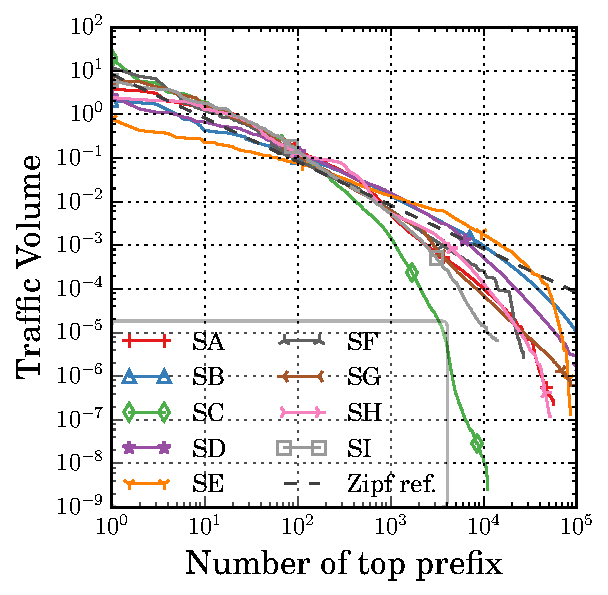
\includegraphics[width=\textwidth]{gfx/chap2/loglog_multi_site.pdf}
                \caption{Week volume share, log-log.}
                \label{fig:week_zipf}
        \end{subfigure}  
        \hfill
        \begin{subfigure}[b]{0.49\textwidth}
        		\centering
                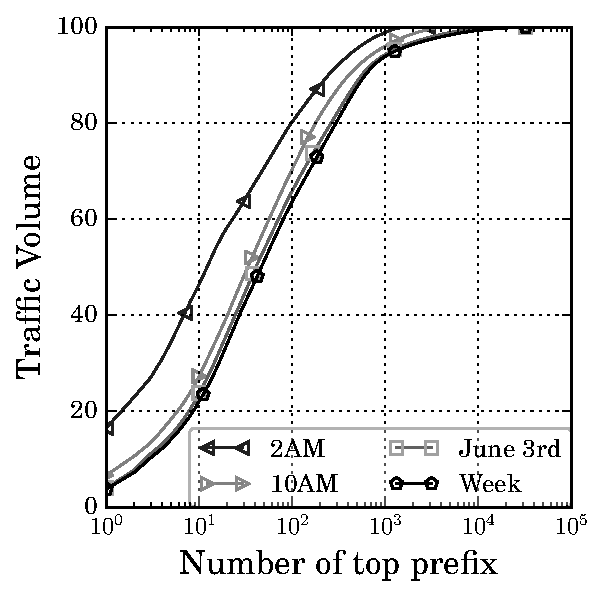
\includegraphics[width=\textwidth]{gfx/chap2/cdf_multi_time.pdf}
                \caption{CDF, different time spans, SA.}
                \label{fig:sa_cdf_multi_time}
        \end{subfigure}    
\caption{Traffic distribution among BGP prefixes.}\label{fig:traffic_dis_site}
\end{figure}

As outlined earlier, the feasibility of prefix selection is based on the fundamental assumption that most traffic concentrates on a few popular destinations, as some previous work have shown \cite{Fang1999,Feamster2003, Wallerich2006}. For the sake of reliability, we quickly verify that our dataset demonstrates as well this property of uneven traffic distribution among destination prefixes.

In Fig.~\ref{fig:week_zipf}, the week volume share of each BGP prefix is represented starting from June 1st.
Prefixes are decreasingly sorted along the X-axis according to their cumulative volume fraction over the week.
We observe that the week volume associated with BGP prefixes can be approximately described by a reference Zipf's distribution with $N=10^5, s=1$ (dashed line).\footnote{Zipf's law defines that the $k^{th}$ most popular element among total $N$ elements has an occurrence share of $f(k,s,N)=\frac{1/k^s}{\sum_{n=1}^{N}1/n^s}$.} 
%Wenqin: If this footnote is removed, I'm afraid that the N and s become unclear to readers.
Fig.~\ref{fig:sa_cdf_multi_time} compares the traffic distribution of SA over different time spans: volumes accumulated over one hour, at 2AM and 10AM, traffic accumulated over 24 hours (on June 3rd) and that through out the full week.
As expected, these graphs confirm that Internet traffic is highly concentrated on a few prefixes over multiple different time resolutions, even after years of rapid RIB increase~\cite{potaroo}.
However, Fig.~\ref{fig:sa_cdf_multi_time} demonstrates that the level of traffic concentration over BGP prefixes is not stable but rather varies within a day, which leads to the study in the following section.

\subsection{Temporal dynamism of traffic over BGP prefixes}
\label{sec:dyna}

\subsubsection{Coefficient of Variation}

Each destination prefix $P$ ever active during a week is associated with a time series $v(P)={\left\{ v(P)_h\right\} }_{h=1, \dots, 168}$ that
stores its traffic volume over the week at hour interval. 
We define the Coefficient of Variation ($c_v$) for prefix $P$'s hour volume series over the week as
\begin{equation*}
c_v(P) = \frac{\delta(v(P))}{\mu(v(P))},
\label{eq:cv}
\end{equation*}
where $\delta$ denotes the standard deviation of the hour volume series and $\mu$ is the mean hour volume over the week.
$c_v$ is a measure of traffic volume variation in relation to its hourly mean over a week.
A large $c_v(P)$ value indicates a large range of variation w.r.t. its average level, and consequently more difficult to anticipate the traffic volumes for this prefix $P$~\cite{He2005}.\footnote{By construction, the maximum $c_v$ for a hourly volume series of 168 in length is $\sqrt{167}$, corresponding to the case where the prefix in question is active during only one single hour throughout the entire week.}

\begin{figure}[!htb]
\centering
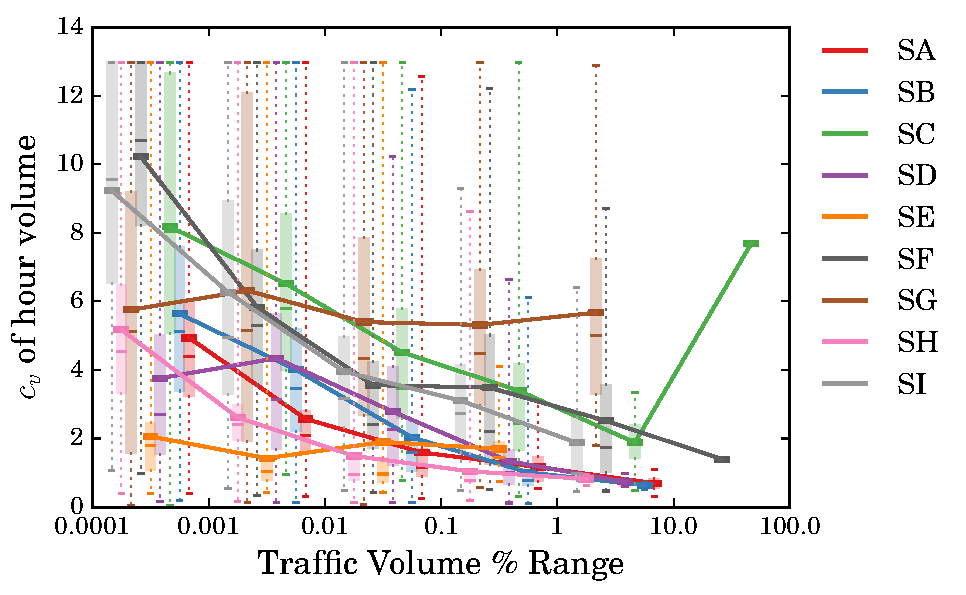
\includegraphics[width=1\textwidth]{gfx/chap2/cv_bin.pdf}
\caption{Relation between $\{c_v(P)\}_P$  and  fraction of weekly volume for all BGP prefixes $P$. 
}
\label{fig:cv}
\end{figure}

Fig.~\ref{fig:cv} depicts the relation between the coefficient of variation and the volume ``importance'' of the prefix over a week. For each prefix $P$,  the X-axis corresponds to its fraction of volume over the week, grouped in six bins in percentage: $[10^{-4}, 10^{-3})$, $\dots$, to $[10,100)$. Along the Y-axis, we use a  box-plot to describe the $c_v$ distribution for prefixes within each bin, mean, median, 25-75 percentile.
We observe that, for all the networks except SG and SE, $c_v$ of large volume prefixes tends to be smaller in average and constrained in a narrower box. On the contrary, the prefixes with smaller week volume tend to have larger coefficient of variation. 
This is an interesting property, as it allows us to capture a significant part of the overall traffic (represented by these stable prefixes) by simply selecting the prefixes with large average hour volume. 

\subsubsection{\textit{Core} presence intensity}

We describe traffic dynamism from another perspective:
for each hour $h$, we define the $core_h$ as the set containing top prefixes that represent $95\%$ of total traffic. 
Table~\ref{tab:core_size} lists the average number of prefixes included in the \textit{core} and its percentage with regard to the average number of active prefixes each hour. 

\begin{table}[!htb]
\centering
\begin{tabular}{cccc}\toprule
\textbf{Name} & \textbf{Avg. prefix \#} & \textbf{Avg. prefix $\%$} & \textbf{Max prefix \#}\\
\midrule
SA & 629  & 17.87  & 1051\\
SB & 5264 & 9.45  & 13934\\
SC & 73  & 4.59    & 177\\
SD & 2481  & 17.35 & 3757\\
SE & 15501  & 53.61 & 20900\\
SF & 377  & 30.73    & 772\\
SG & 570 & 7.76    & 1766\\
SH & 965  & 19.42   & 1731\\
SI & 175  & 21.00    & 415\\
\bottomrule
\end{tabular}
\caption{Core prefix set statistics.}
\label{tab:core_size}
\end{table}

If a prefix is inside the \textit{core} at a certain hour, it can be regarded important for bringing a significant amount of traffic.
We thus defined the ``\textit{core} presence'' for a prefix $P$ at each hour $h$ as:
\begin{equation*}
cp(P)_i = \begin{dcases*}
        1  & when $P \in$ $\textit{core}_i$,\\
        0 & otherwise,
        \end{dcases*}
\label{eq:cp}
\end{equation*}
% $cp(P)$ is a time series with which we can further describe the frequency or likelihood of prefix being present in the \textit{core} over the week: 
The \textit{core} presence intensity over one week $I_{cp}(P, 168)$ is then defined as:
$I_{cp}(P,168) = \frac{1}{168} \sum_{i=1}^{168} cp(P)_i$.

\begin{figure}[!tb]
\centering
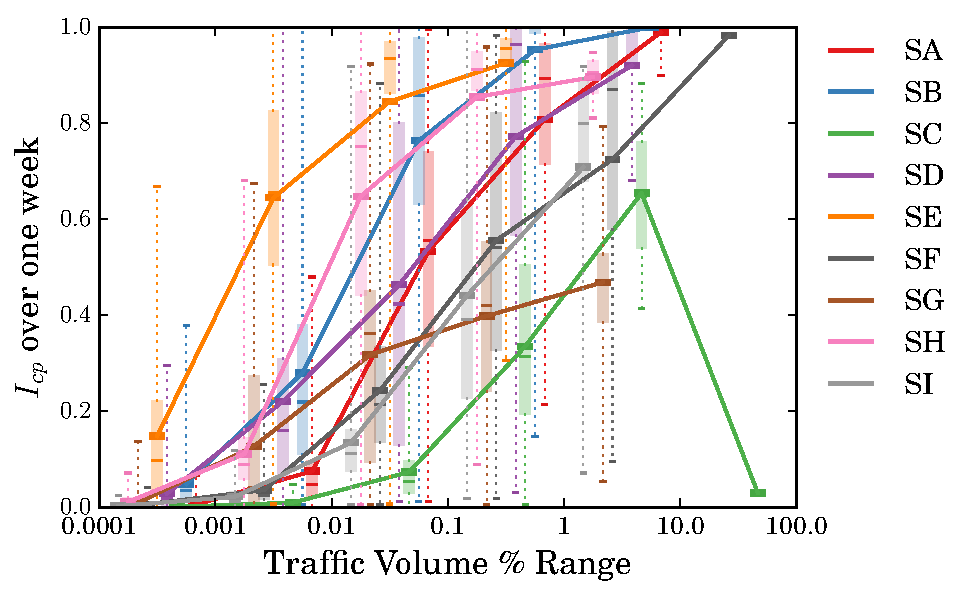
\includegraphics[width=1\textwidth]{gfx/chap2/cp_bin.pdf}
\caption{Relation between $I_{cp}$ over the week and week volume fraction of BGP prefixes.}
\label{fig:cpi}
\end{figure}

Fig.~\ref{fig:cpi} plots the $I_{cp}$ over one week of each prefix (Y-axis) against its week volume fraction (X-axis), using the same presentation as Fig.~\ref{fig:cv} described above.
For all the networks, we can see that prefixes with bigger week volume share are less likely to have a low $I_{cp}$ over the week, i.e. they appear frequently in the \textit{core}.
We can conclude that, by focusing on prefixes that intensively appear in the \textit{core} through the week, we will be able to capture a large part of the prefixes associated with important traffic volume over the week, and thus cover a large part of the overall traffic.

\subsubsection{Relationship between $I_{cp}$ and $c_v$}
\begin{figure}
		\centering
        \begin{subfigure}[b]{0.49\textwidth}
                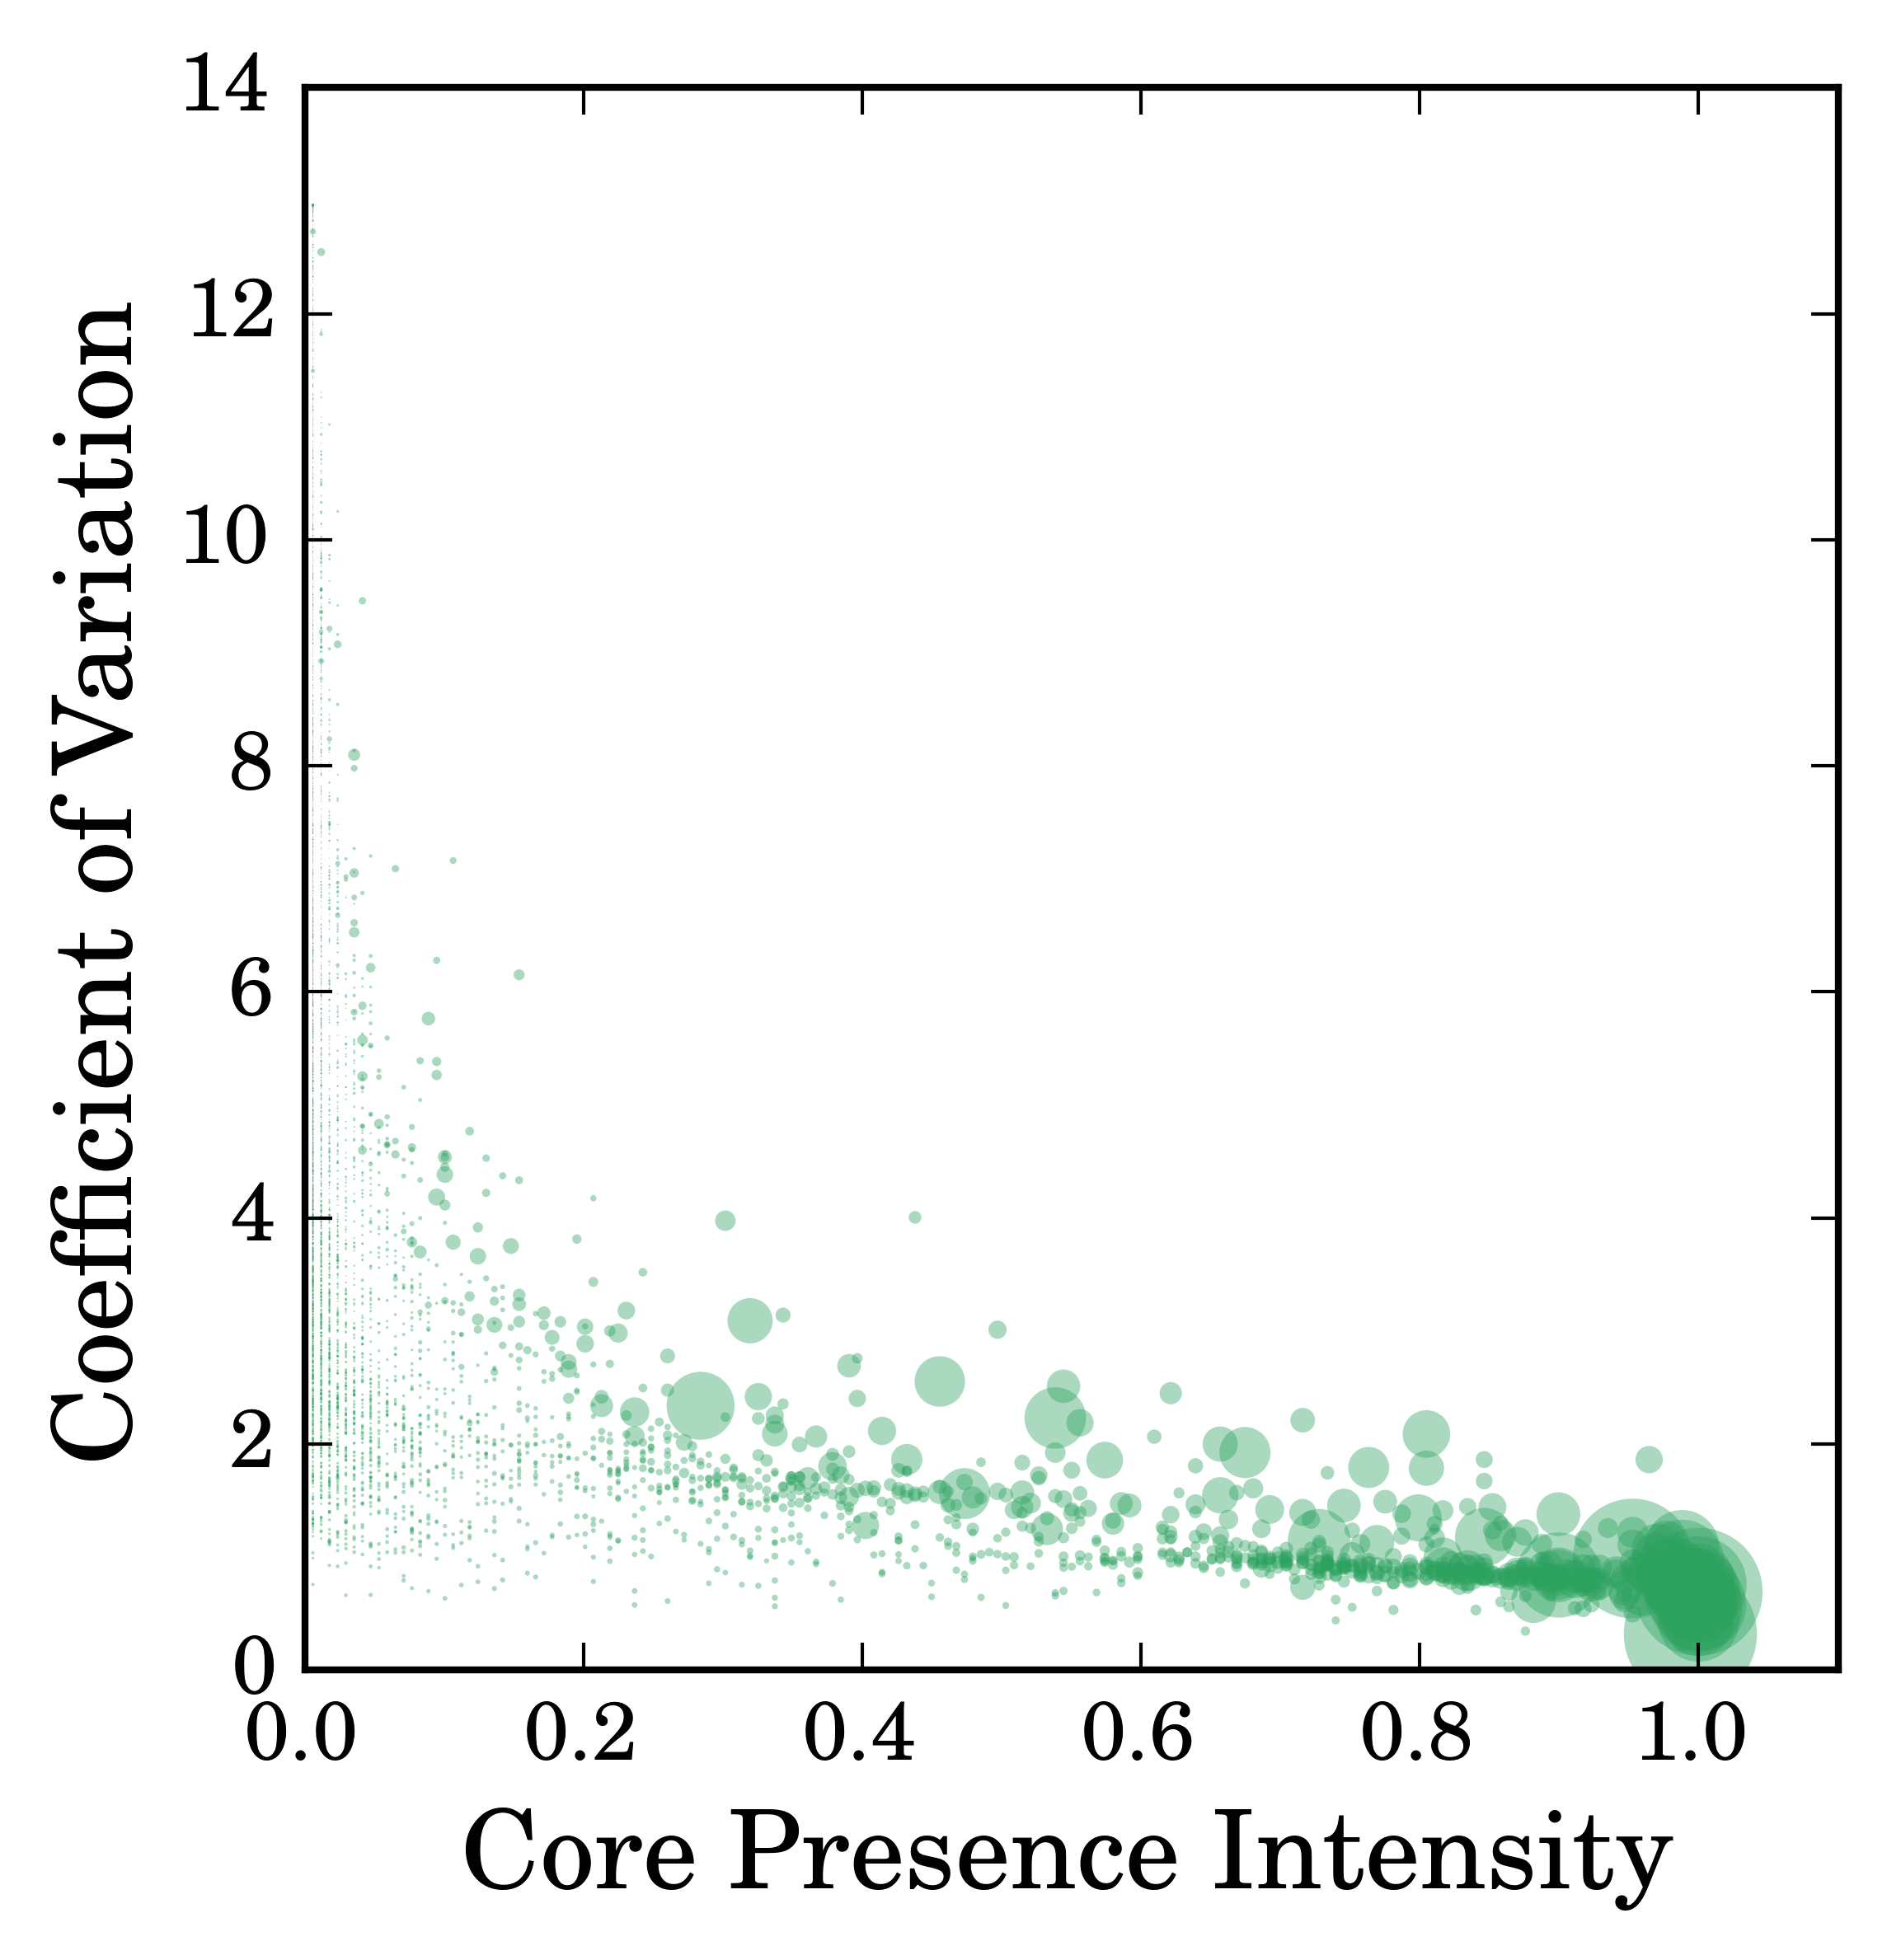
\includegraphics[width=\textwidth]{gfx/chap2/corre_cv_cp_sa.png}
                \caption{SA, 56684 prefixes}
                \label{fig:cv_cp_sa}
        \end{subfigure}
        \begin{subfigure}[b]{0.49\textwidth}
                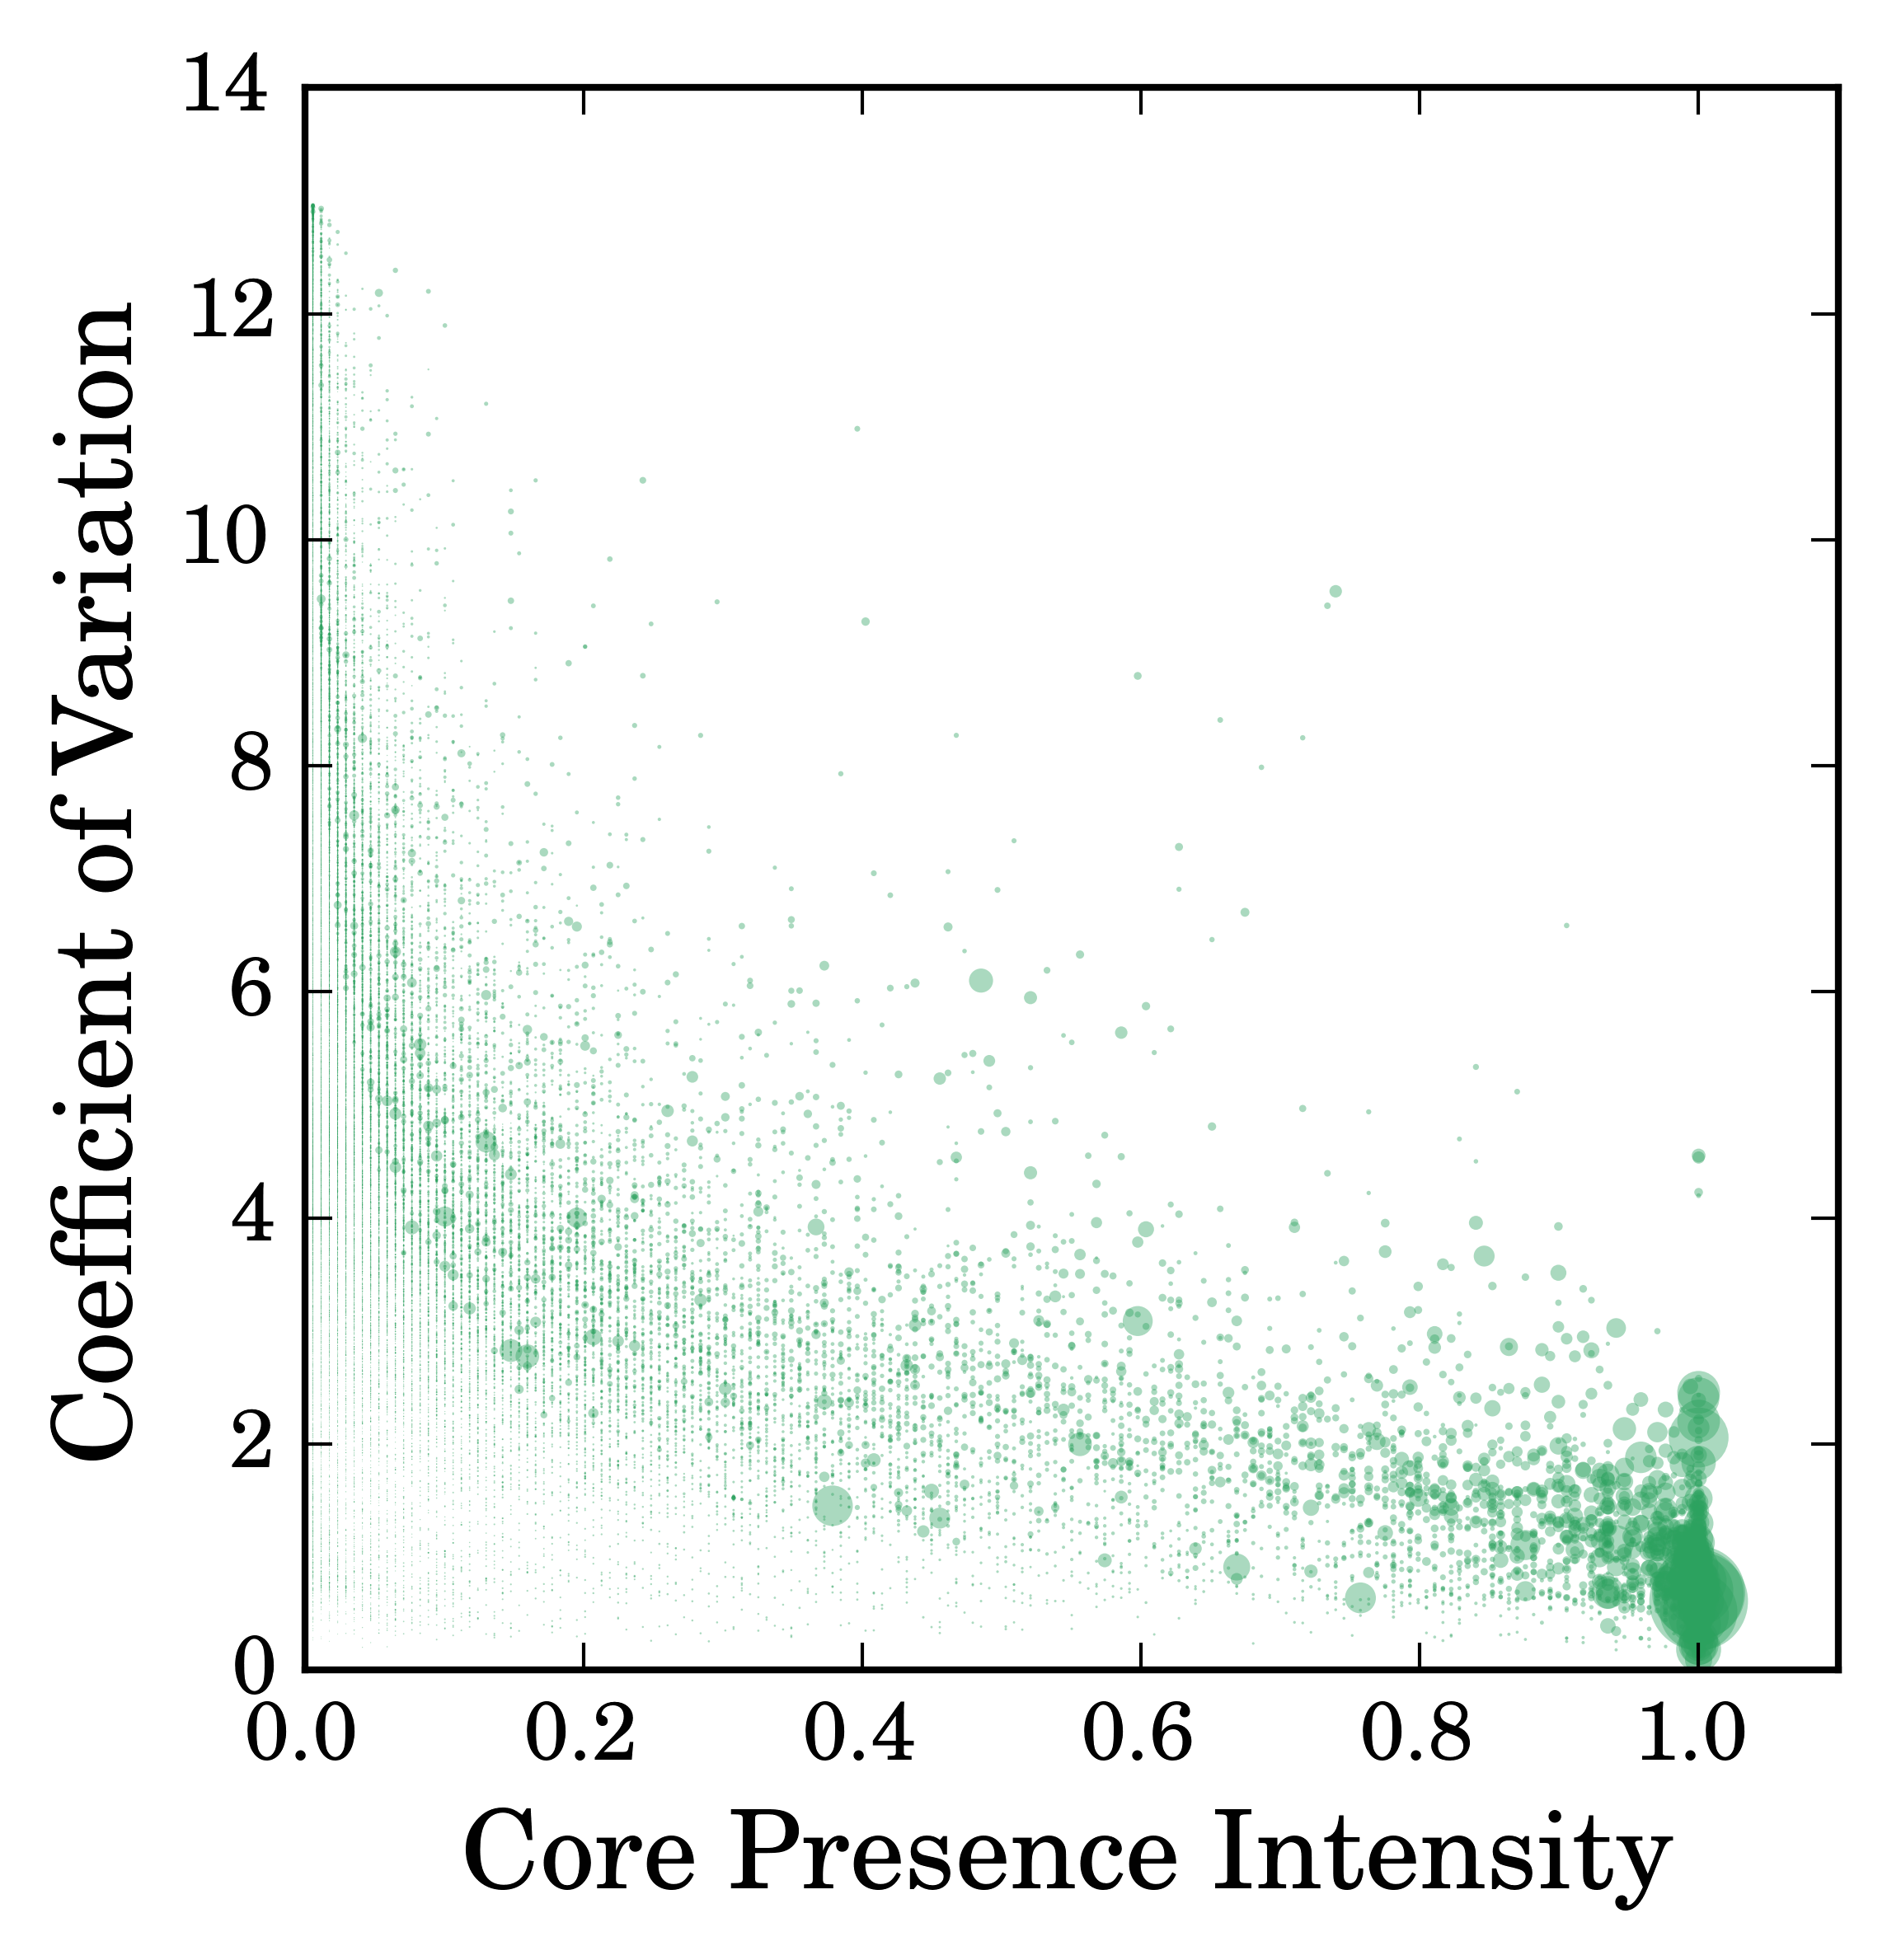
\includegraphics[width=\textwidth]{gfx/chap2/corre_cv_cp_sb.png}
                \caption{SB, 504707 prefixes}
                \label{fig:cv_cp_sb}
        \end{subfigure}
        \begin{subfigure}[b]{0.49\textwidth}
                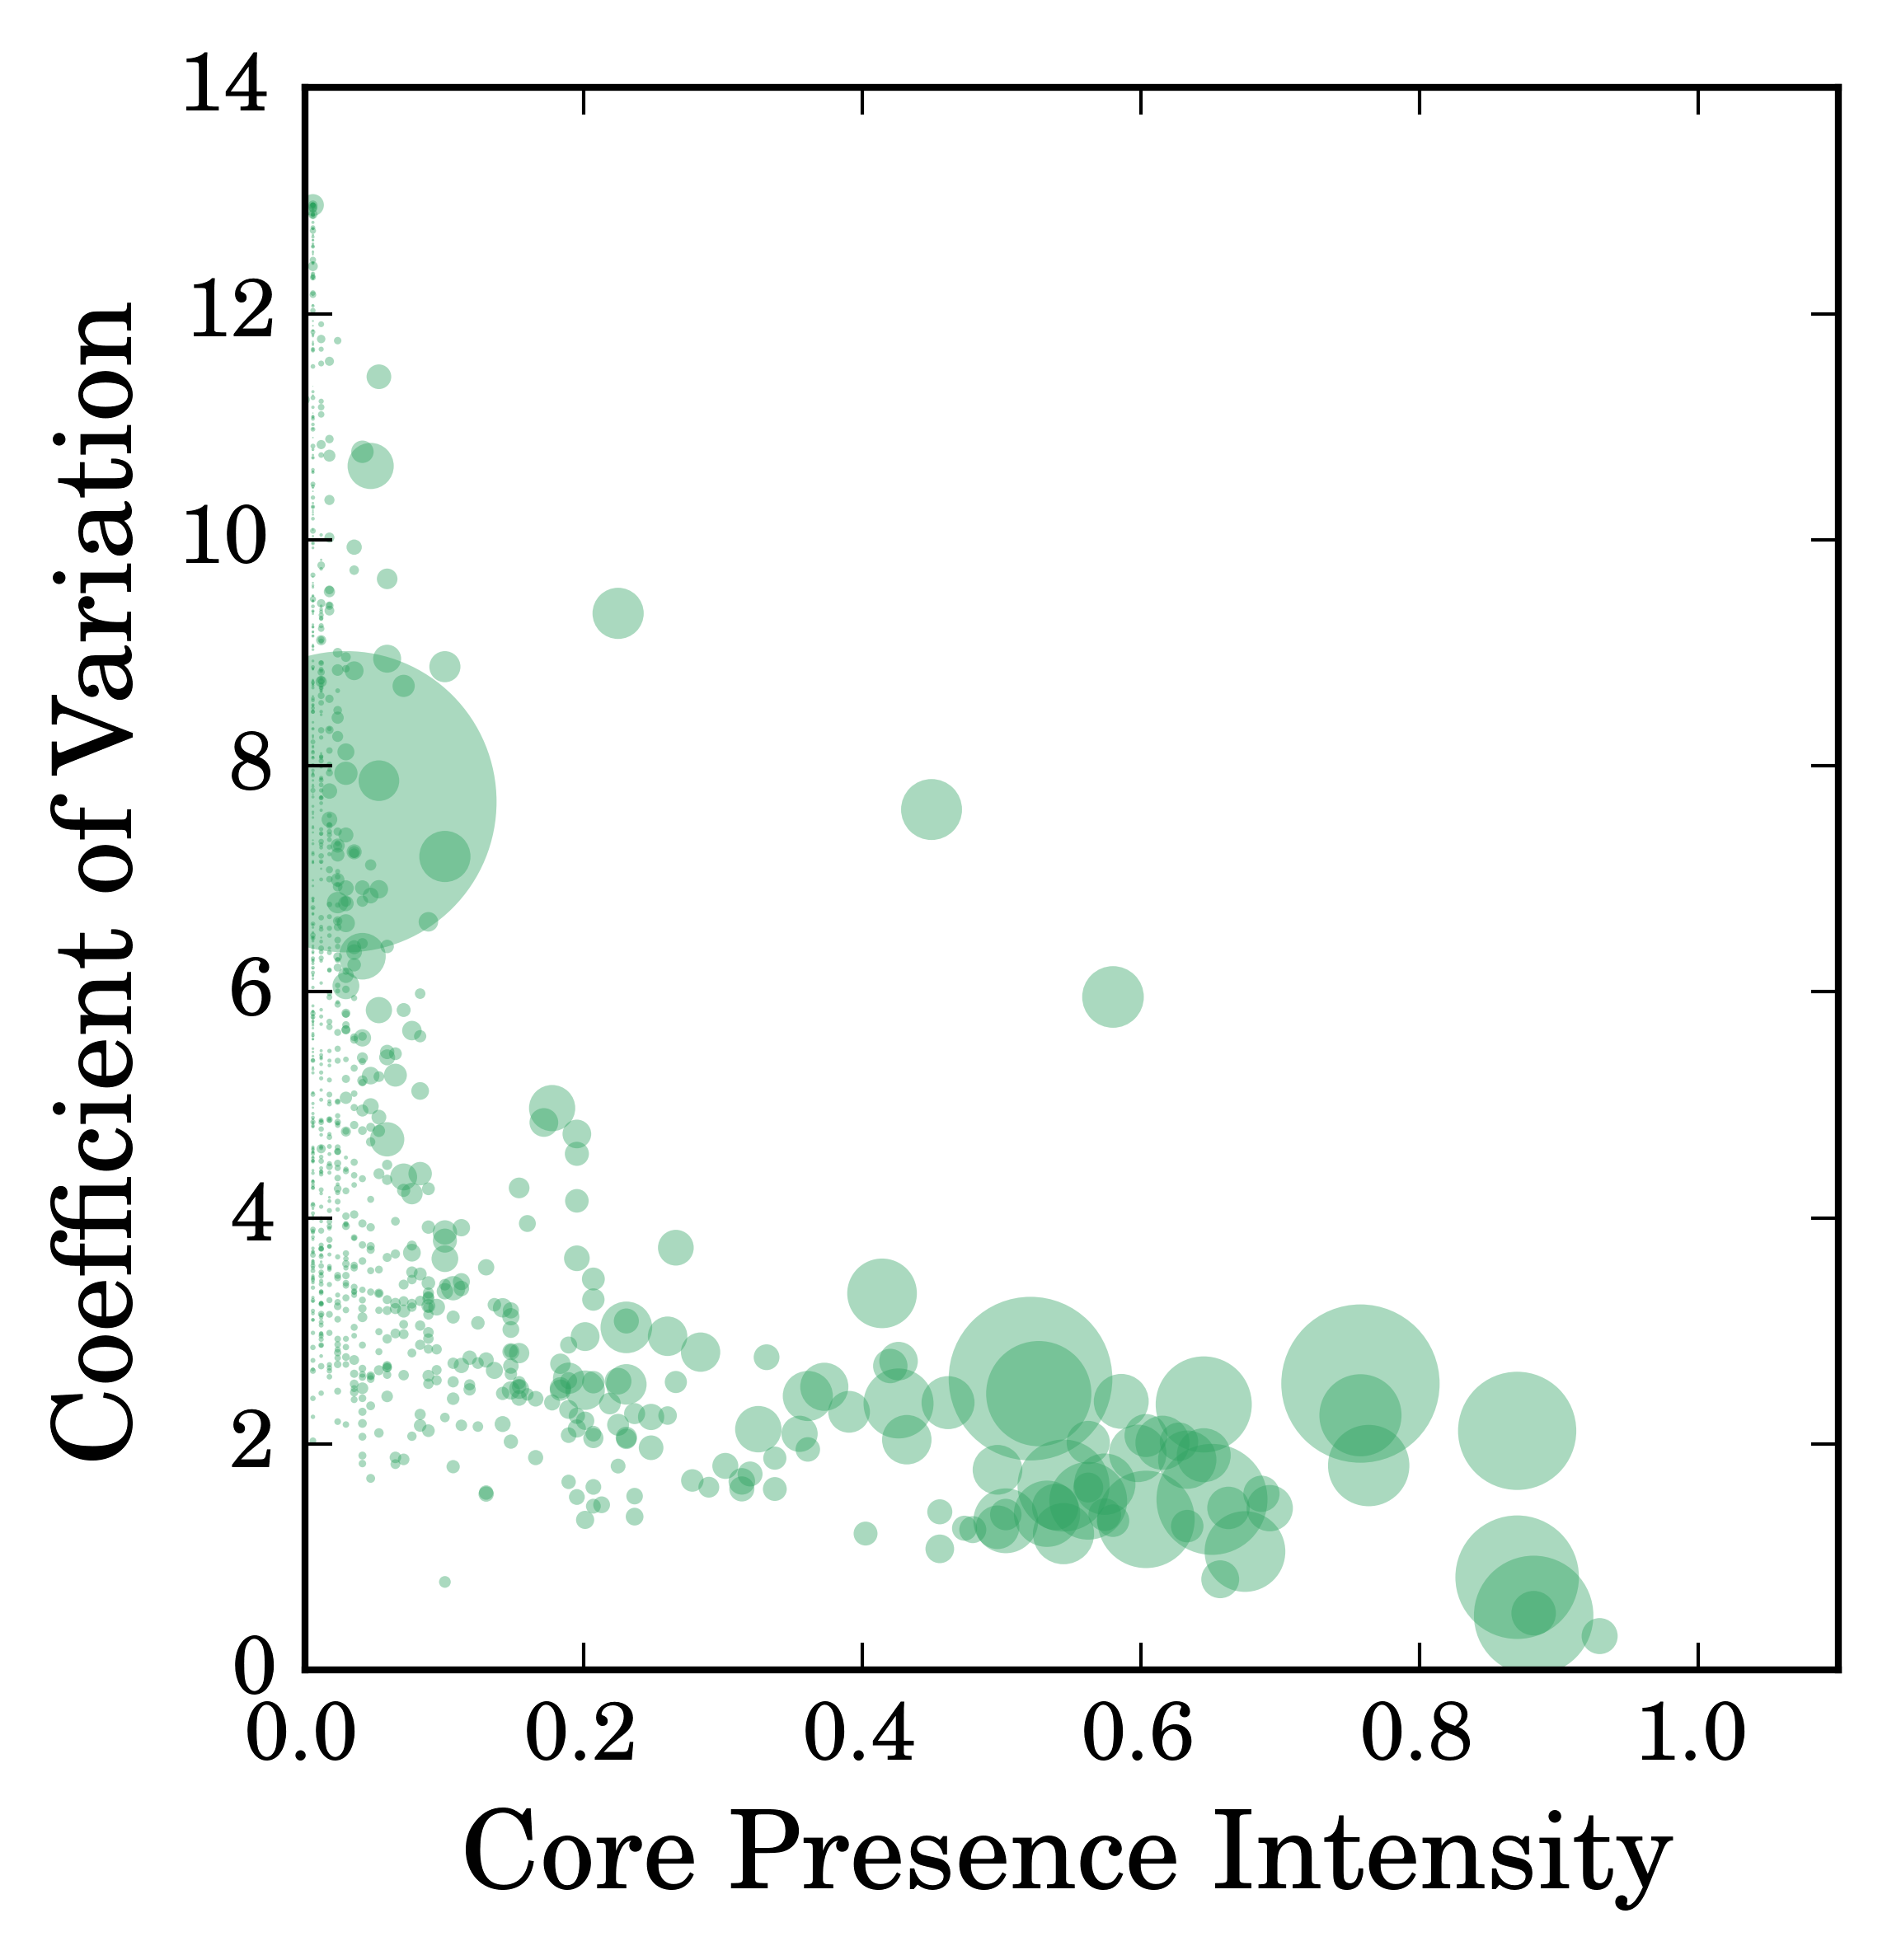
\includegraphics[width=\textwidth]{gfx/chap2/corre_cv_cp_sc.png}
                \caption{SC, 11065 prefixes}
                \label{fig:cv_cp_sc}
        \end{subfigure}
        \begin{subfigure}[b]{0.49\textwidth}
                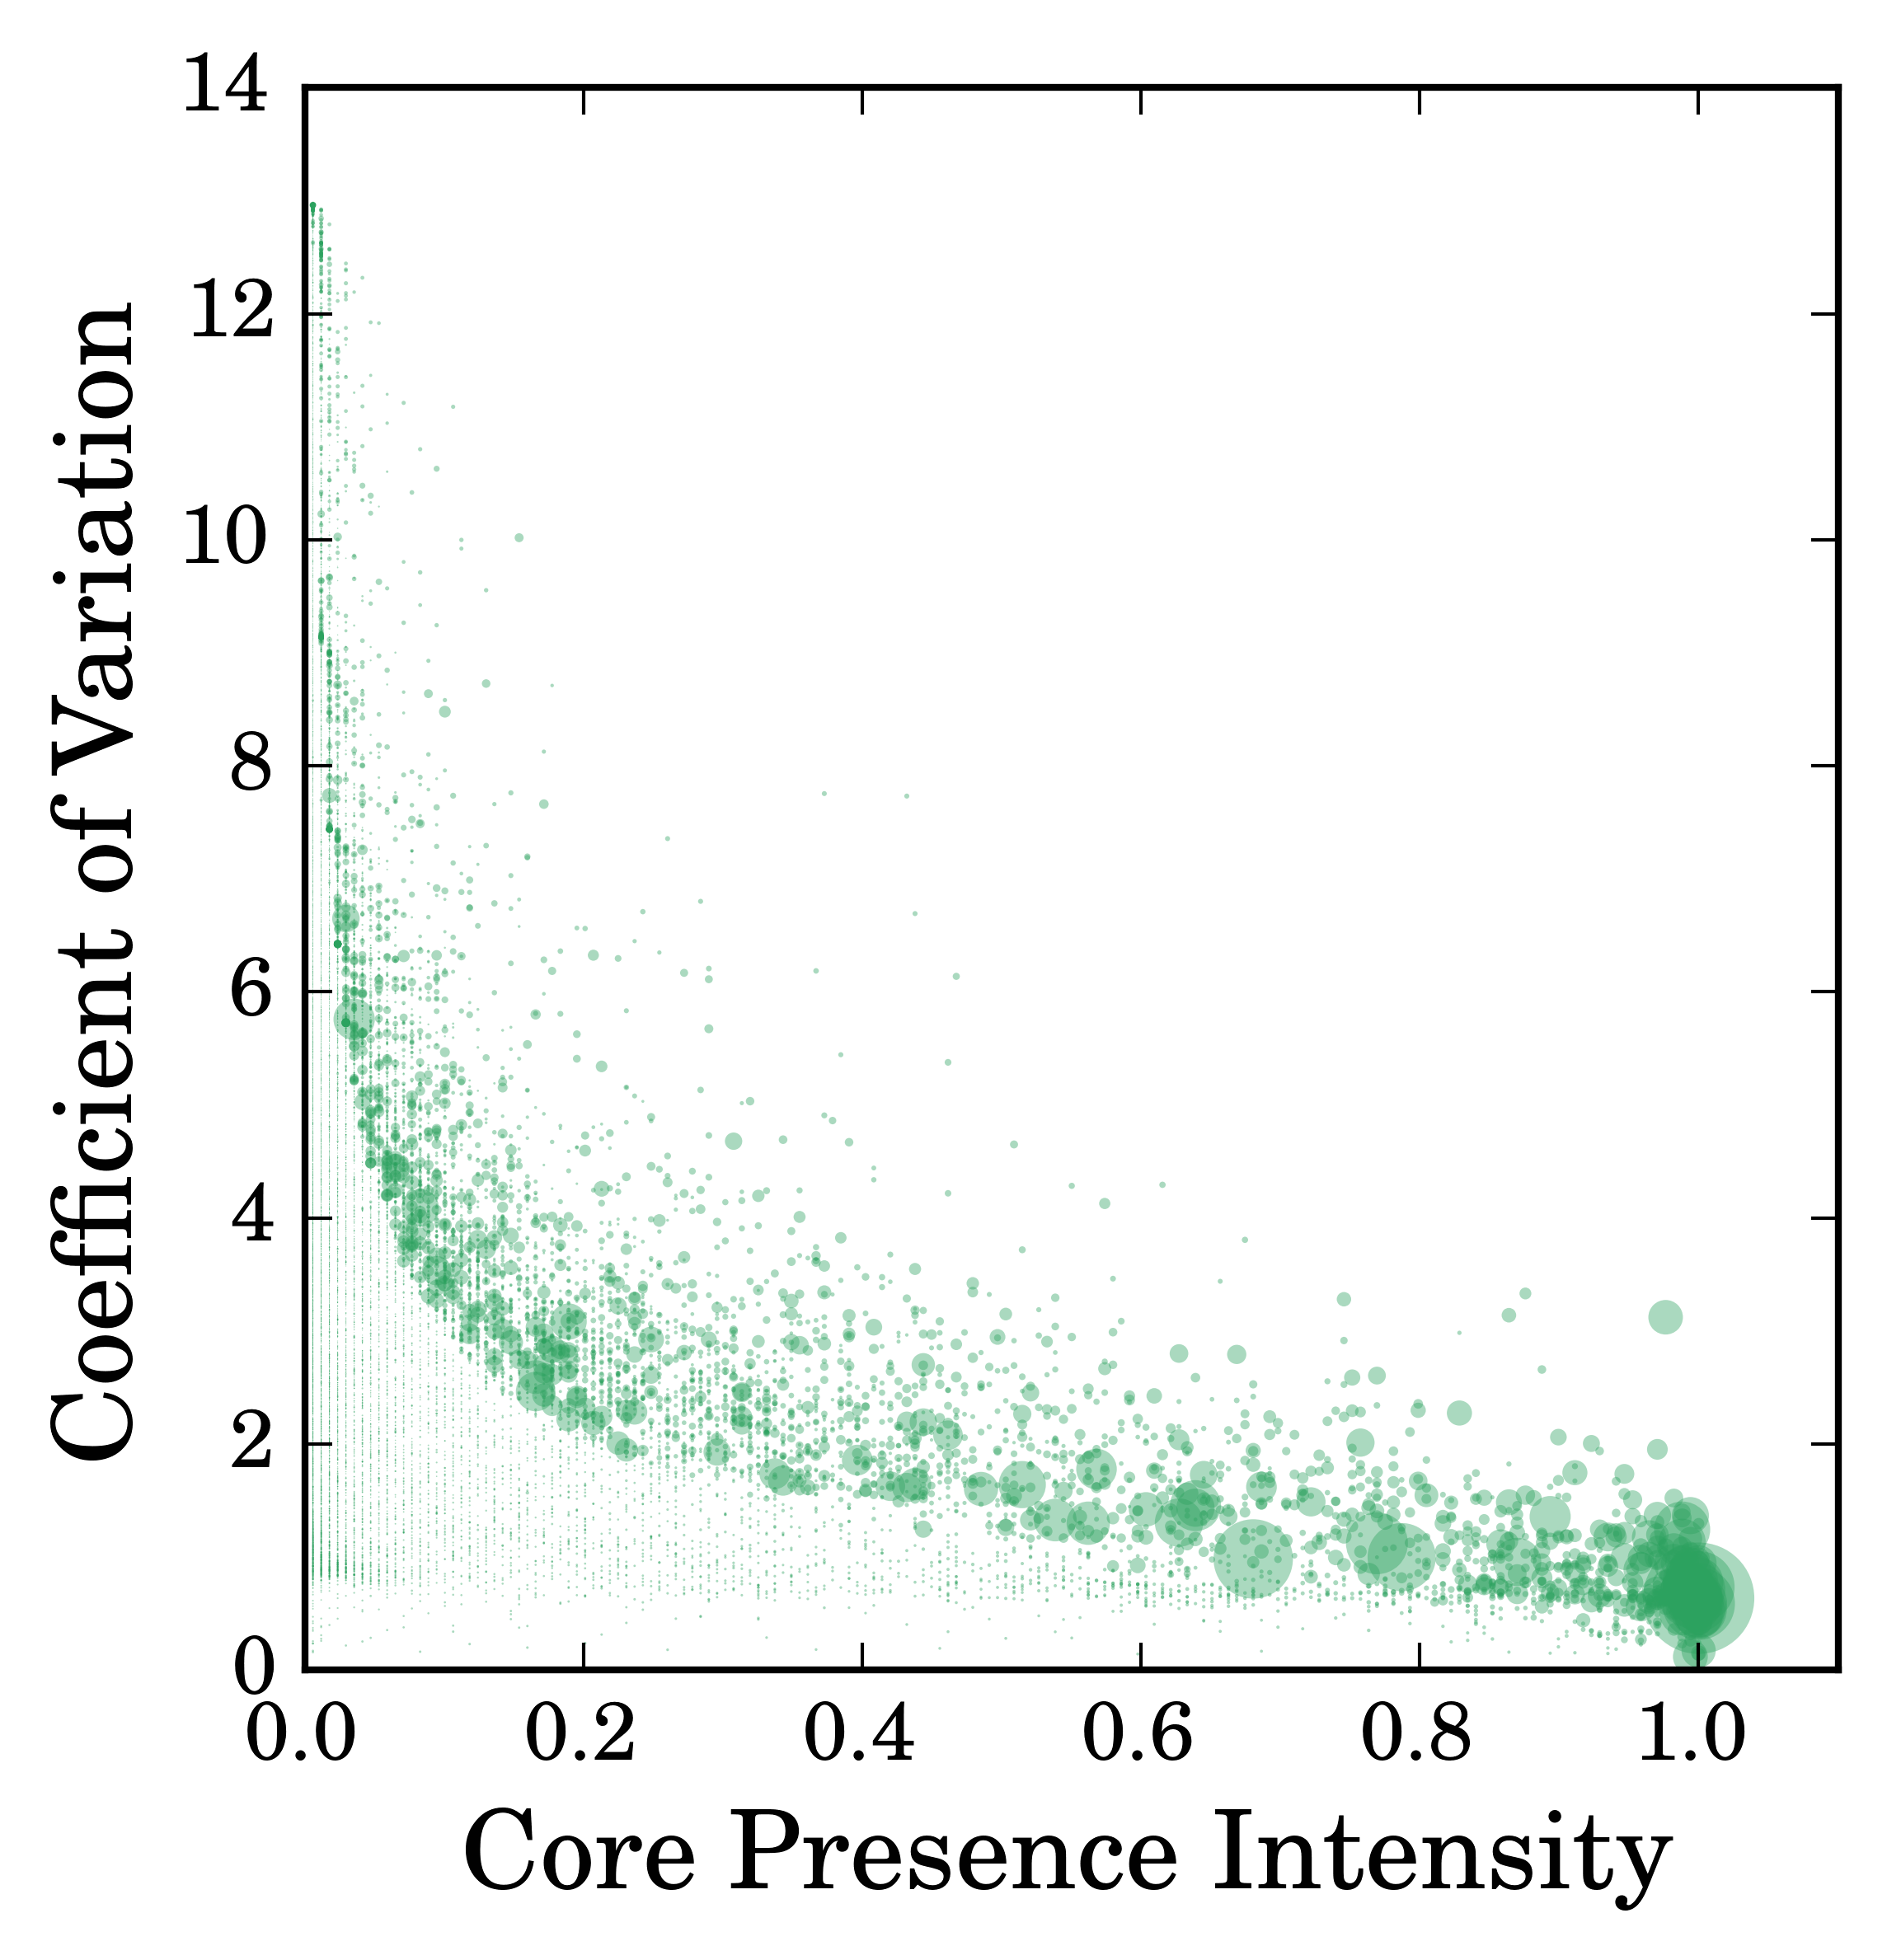
\includegraphics[width=\textwidth]{gfx/chap2/corre_cv_cp_sd.png}
                \caption{SD, 140700 prefixes}
                \label{fig:cv_cp_sd}
        \end{subfigure}
        \begin{subfigure}[b]{0.49\textwidth}
                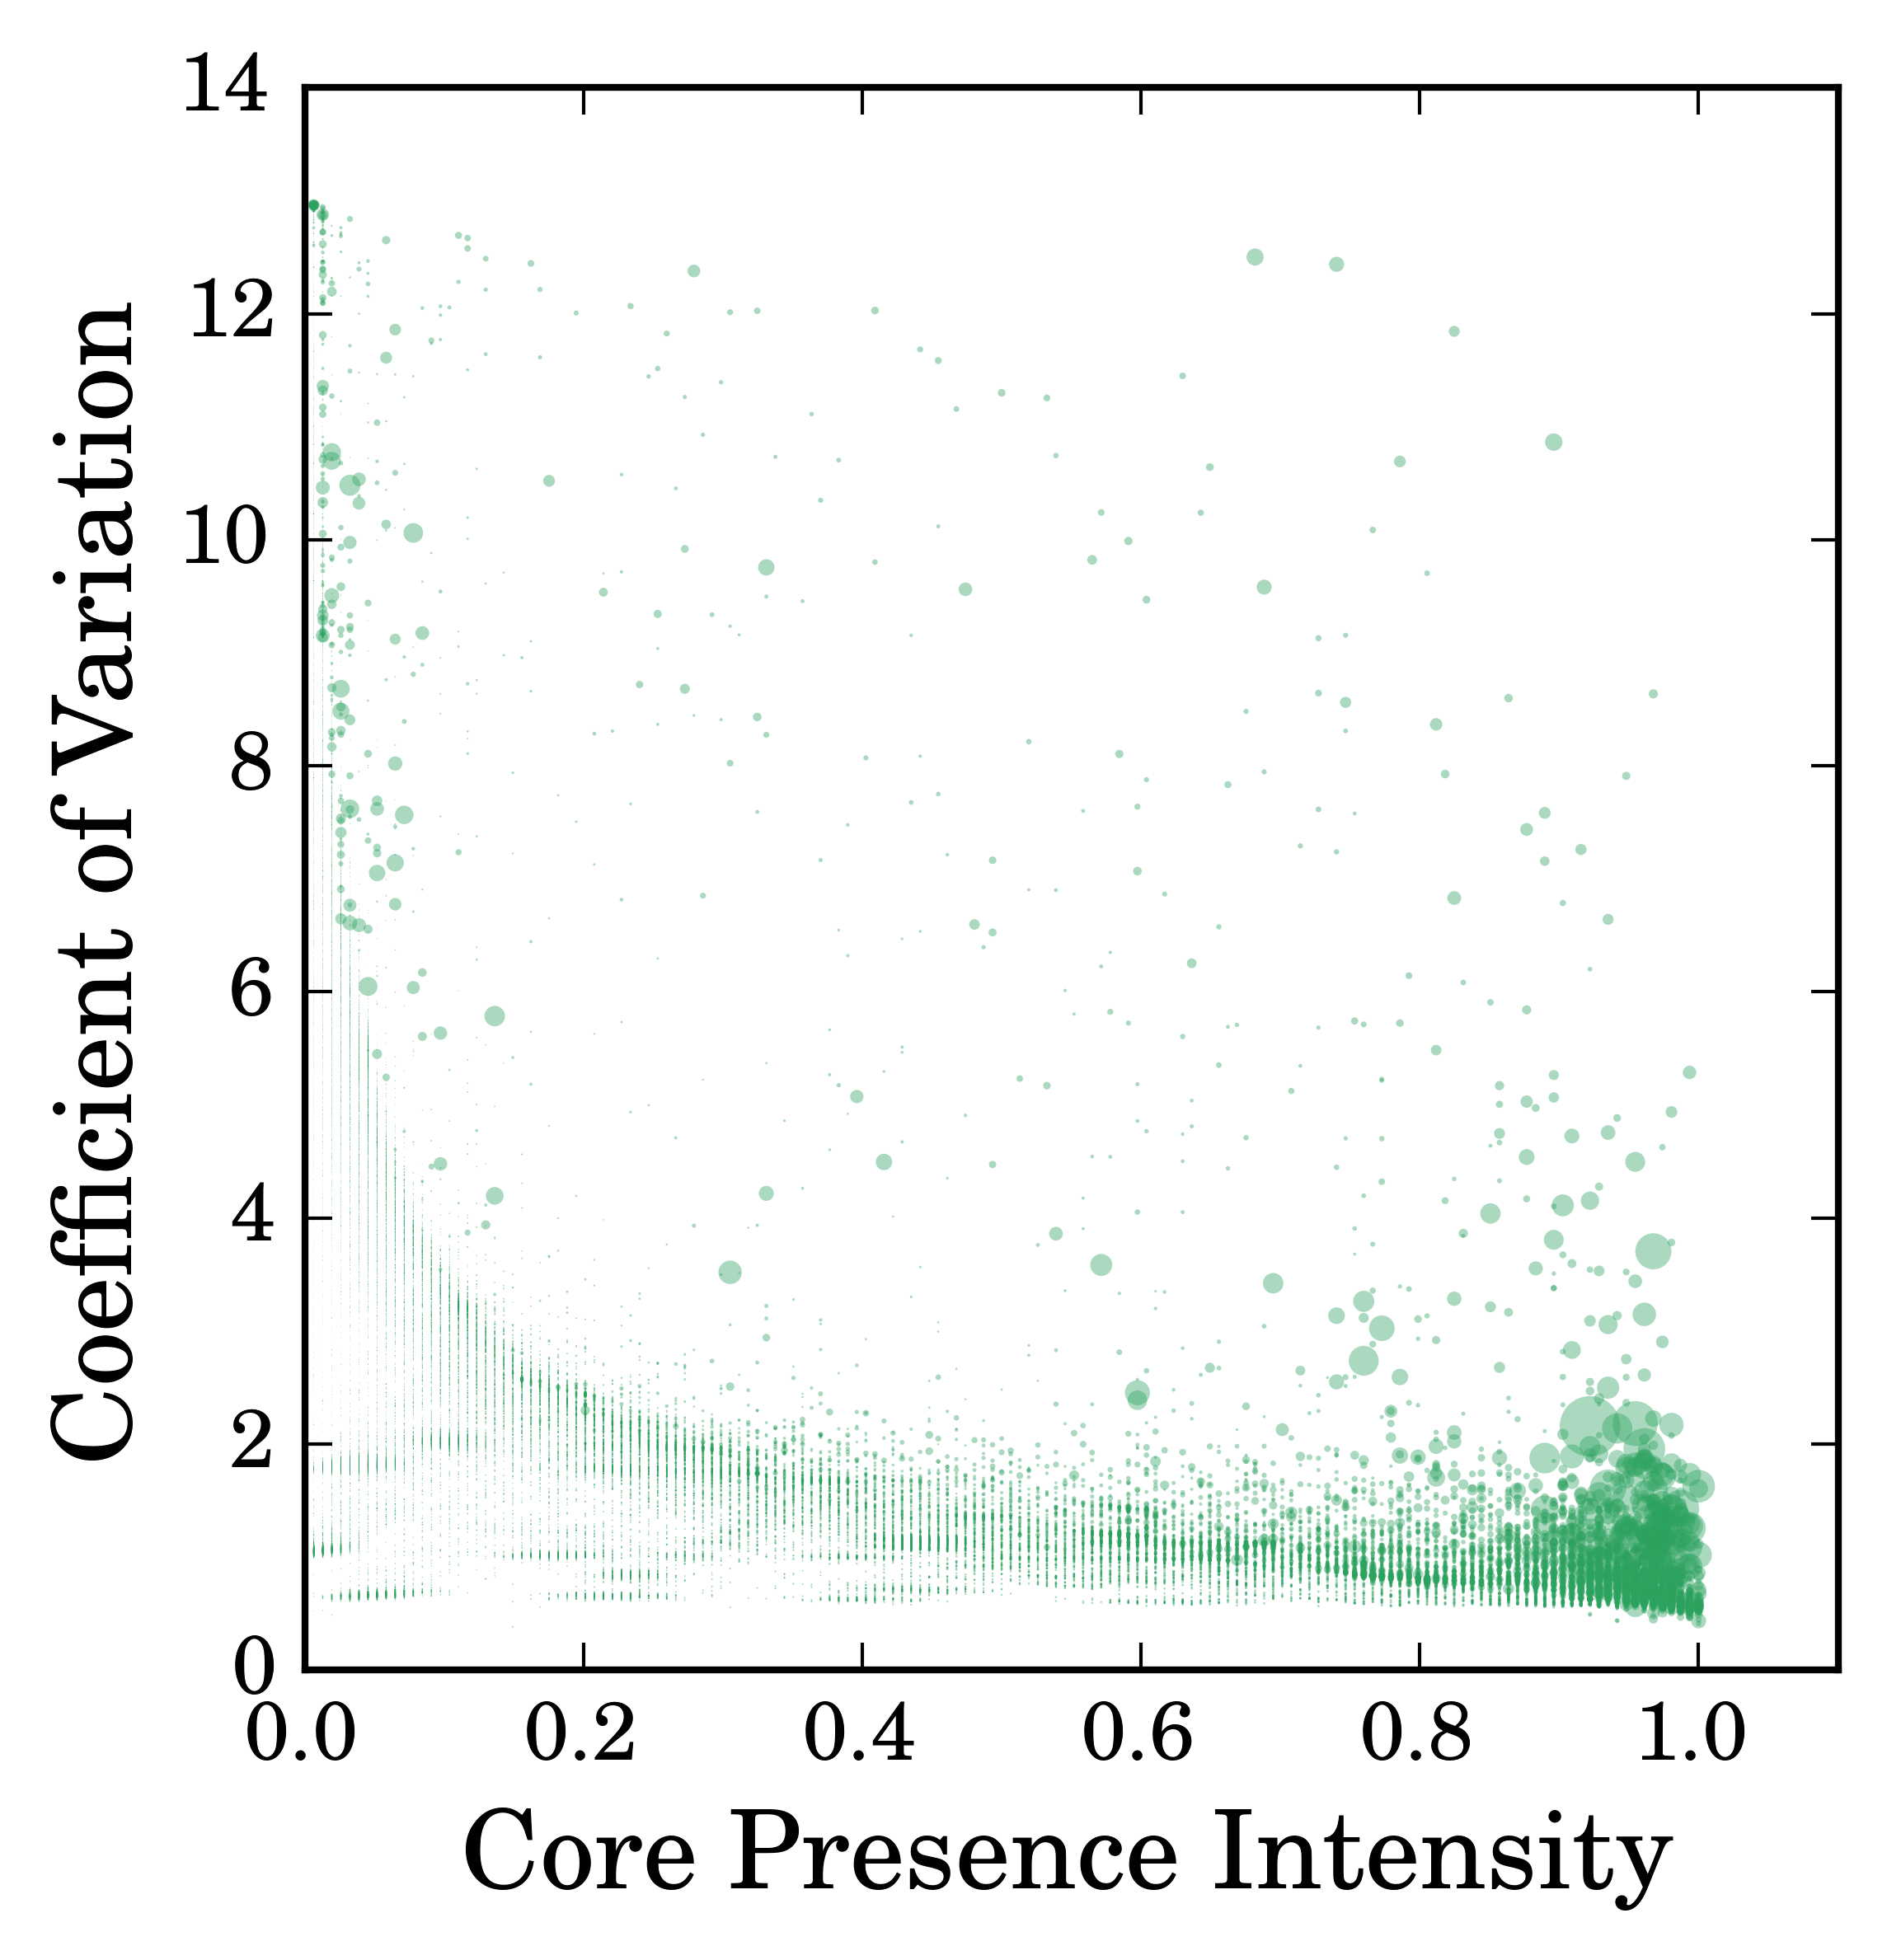
\includegraphics[width=\textwidth]{gfx/chap2/corre_cv_cp_se.png}
                \caption{SE, 86014 prefixes}
                \label{fig:cv_cp_se}
        \end{subfigure}
        \begin{subfigure}[b]{0.49\textwidth}
                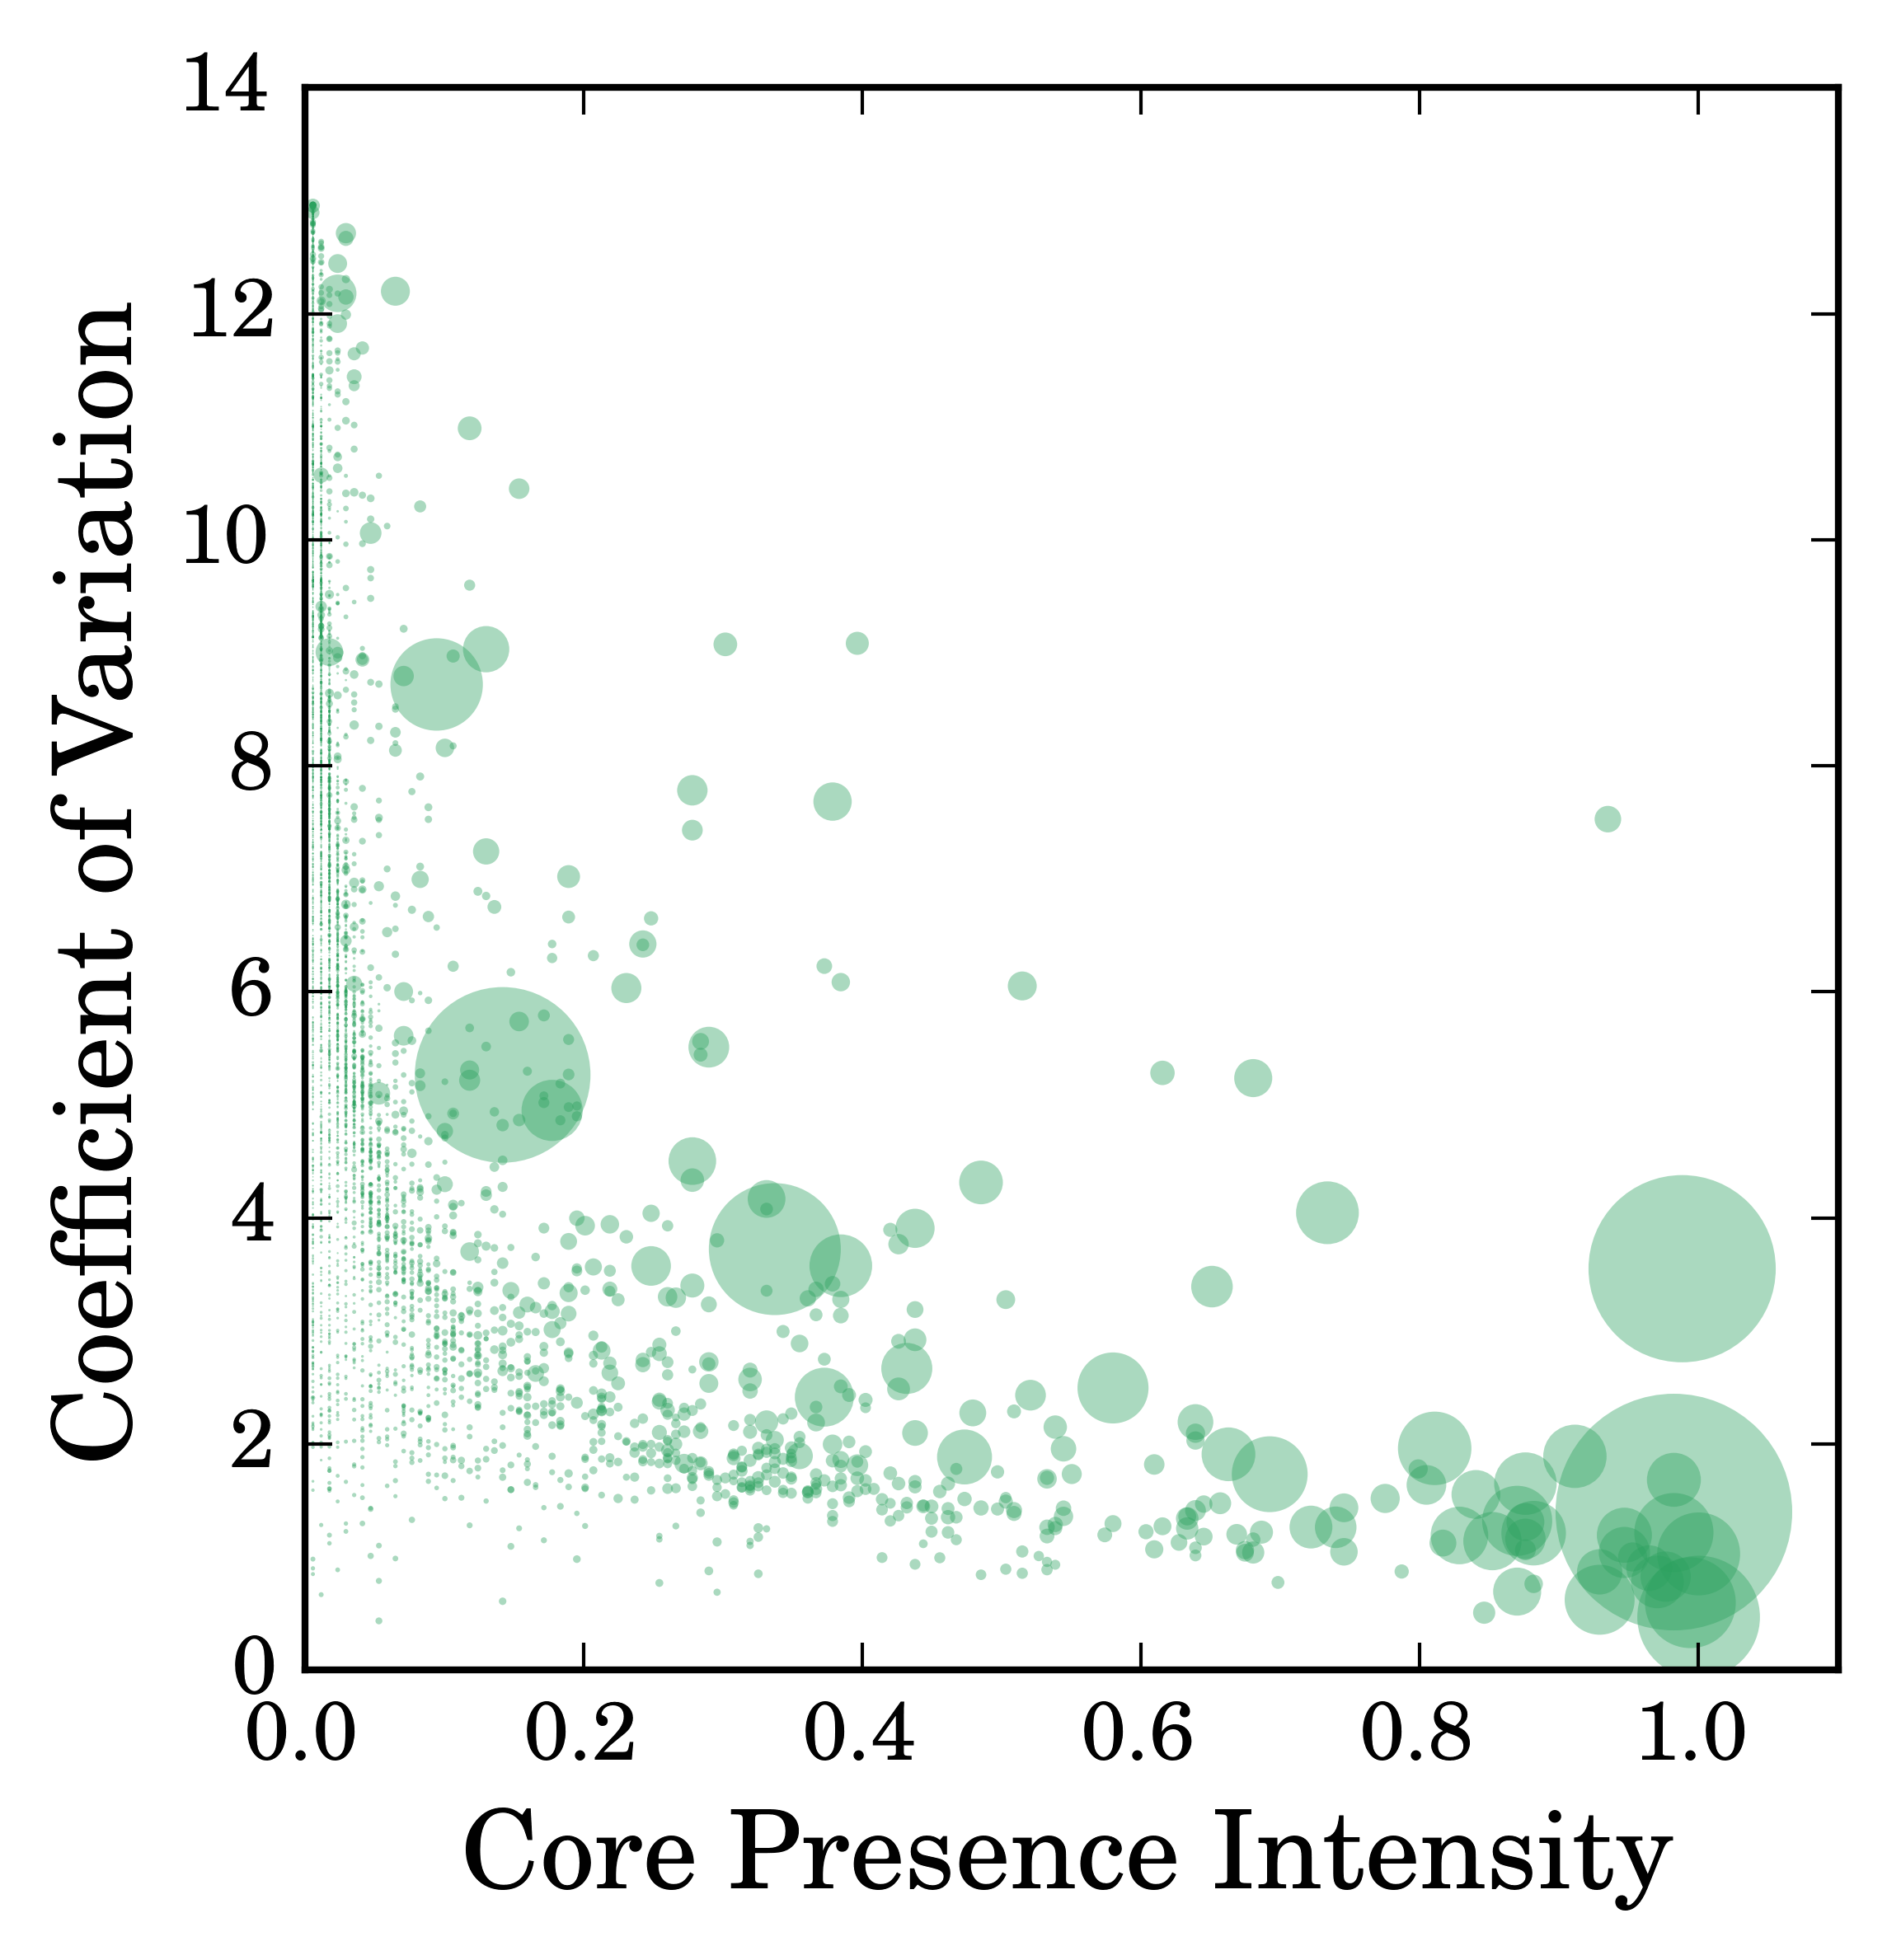
\includegraphics[width=\textwidth]{gfx/chap2/corre_cv_cp_sf.png}
                \caption{SF, 26907 prefixes}
                \label{fig:cv_cp_sf}
        \end{subfigure}
\caption{Relation between $I_{cp}$ over one week and $c_v$ of hour volume over the week from June 1st, 2015. Each circle stands for a prefix. Number of active prefixes plotted is each sub-graph throughout the week is also given. Circle size is proportional to the week volume fraction of the prefix the circle represents and is of the same scale for all networks.}
\label{fig:cv_cp}
\end{figure}
\begin{figure}\ContinuedFloat
        \begin{subfigure}[b]{0.49\textwidth}
                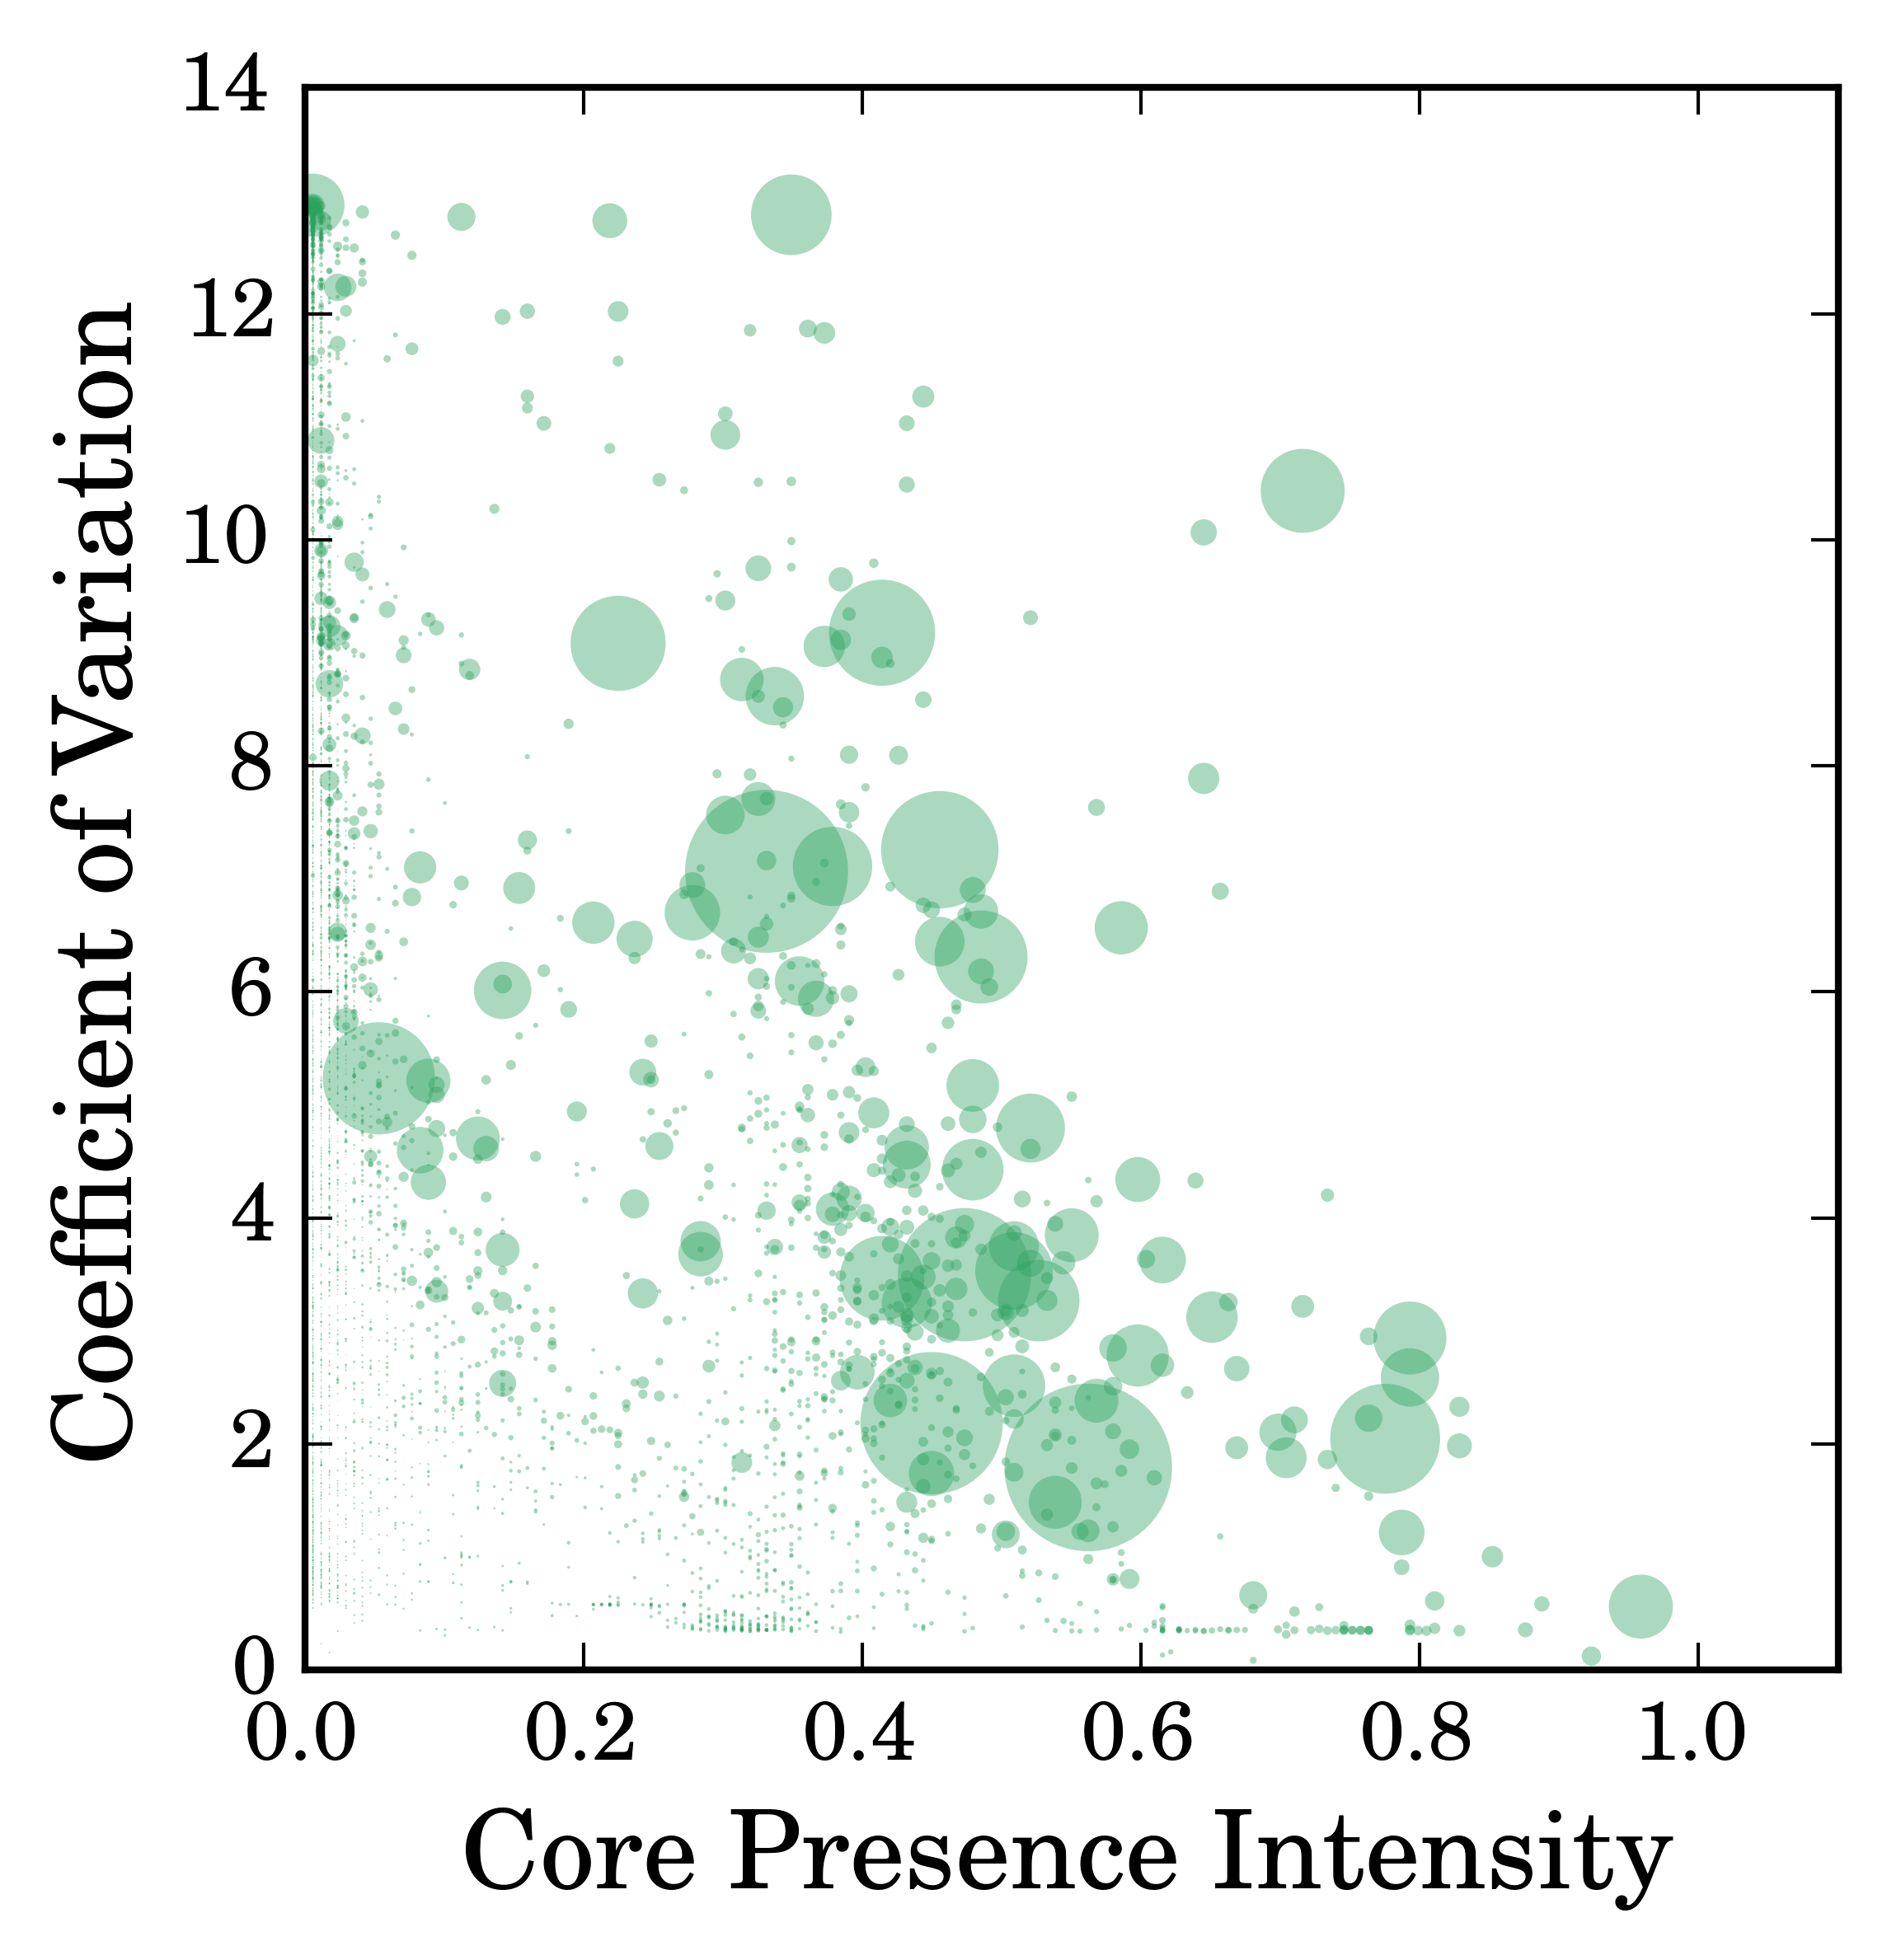
\includegraphics[width=\textwidth]{gfx/chap2/corre_cv_cp_sg.png}
                \caption{SG, 104425 prefixes}
                \label{fig:cv_cp_sg}
        \end{subfigure}
        \begin{subfigure}[b]{0.49\textwidth}
                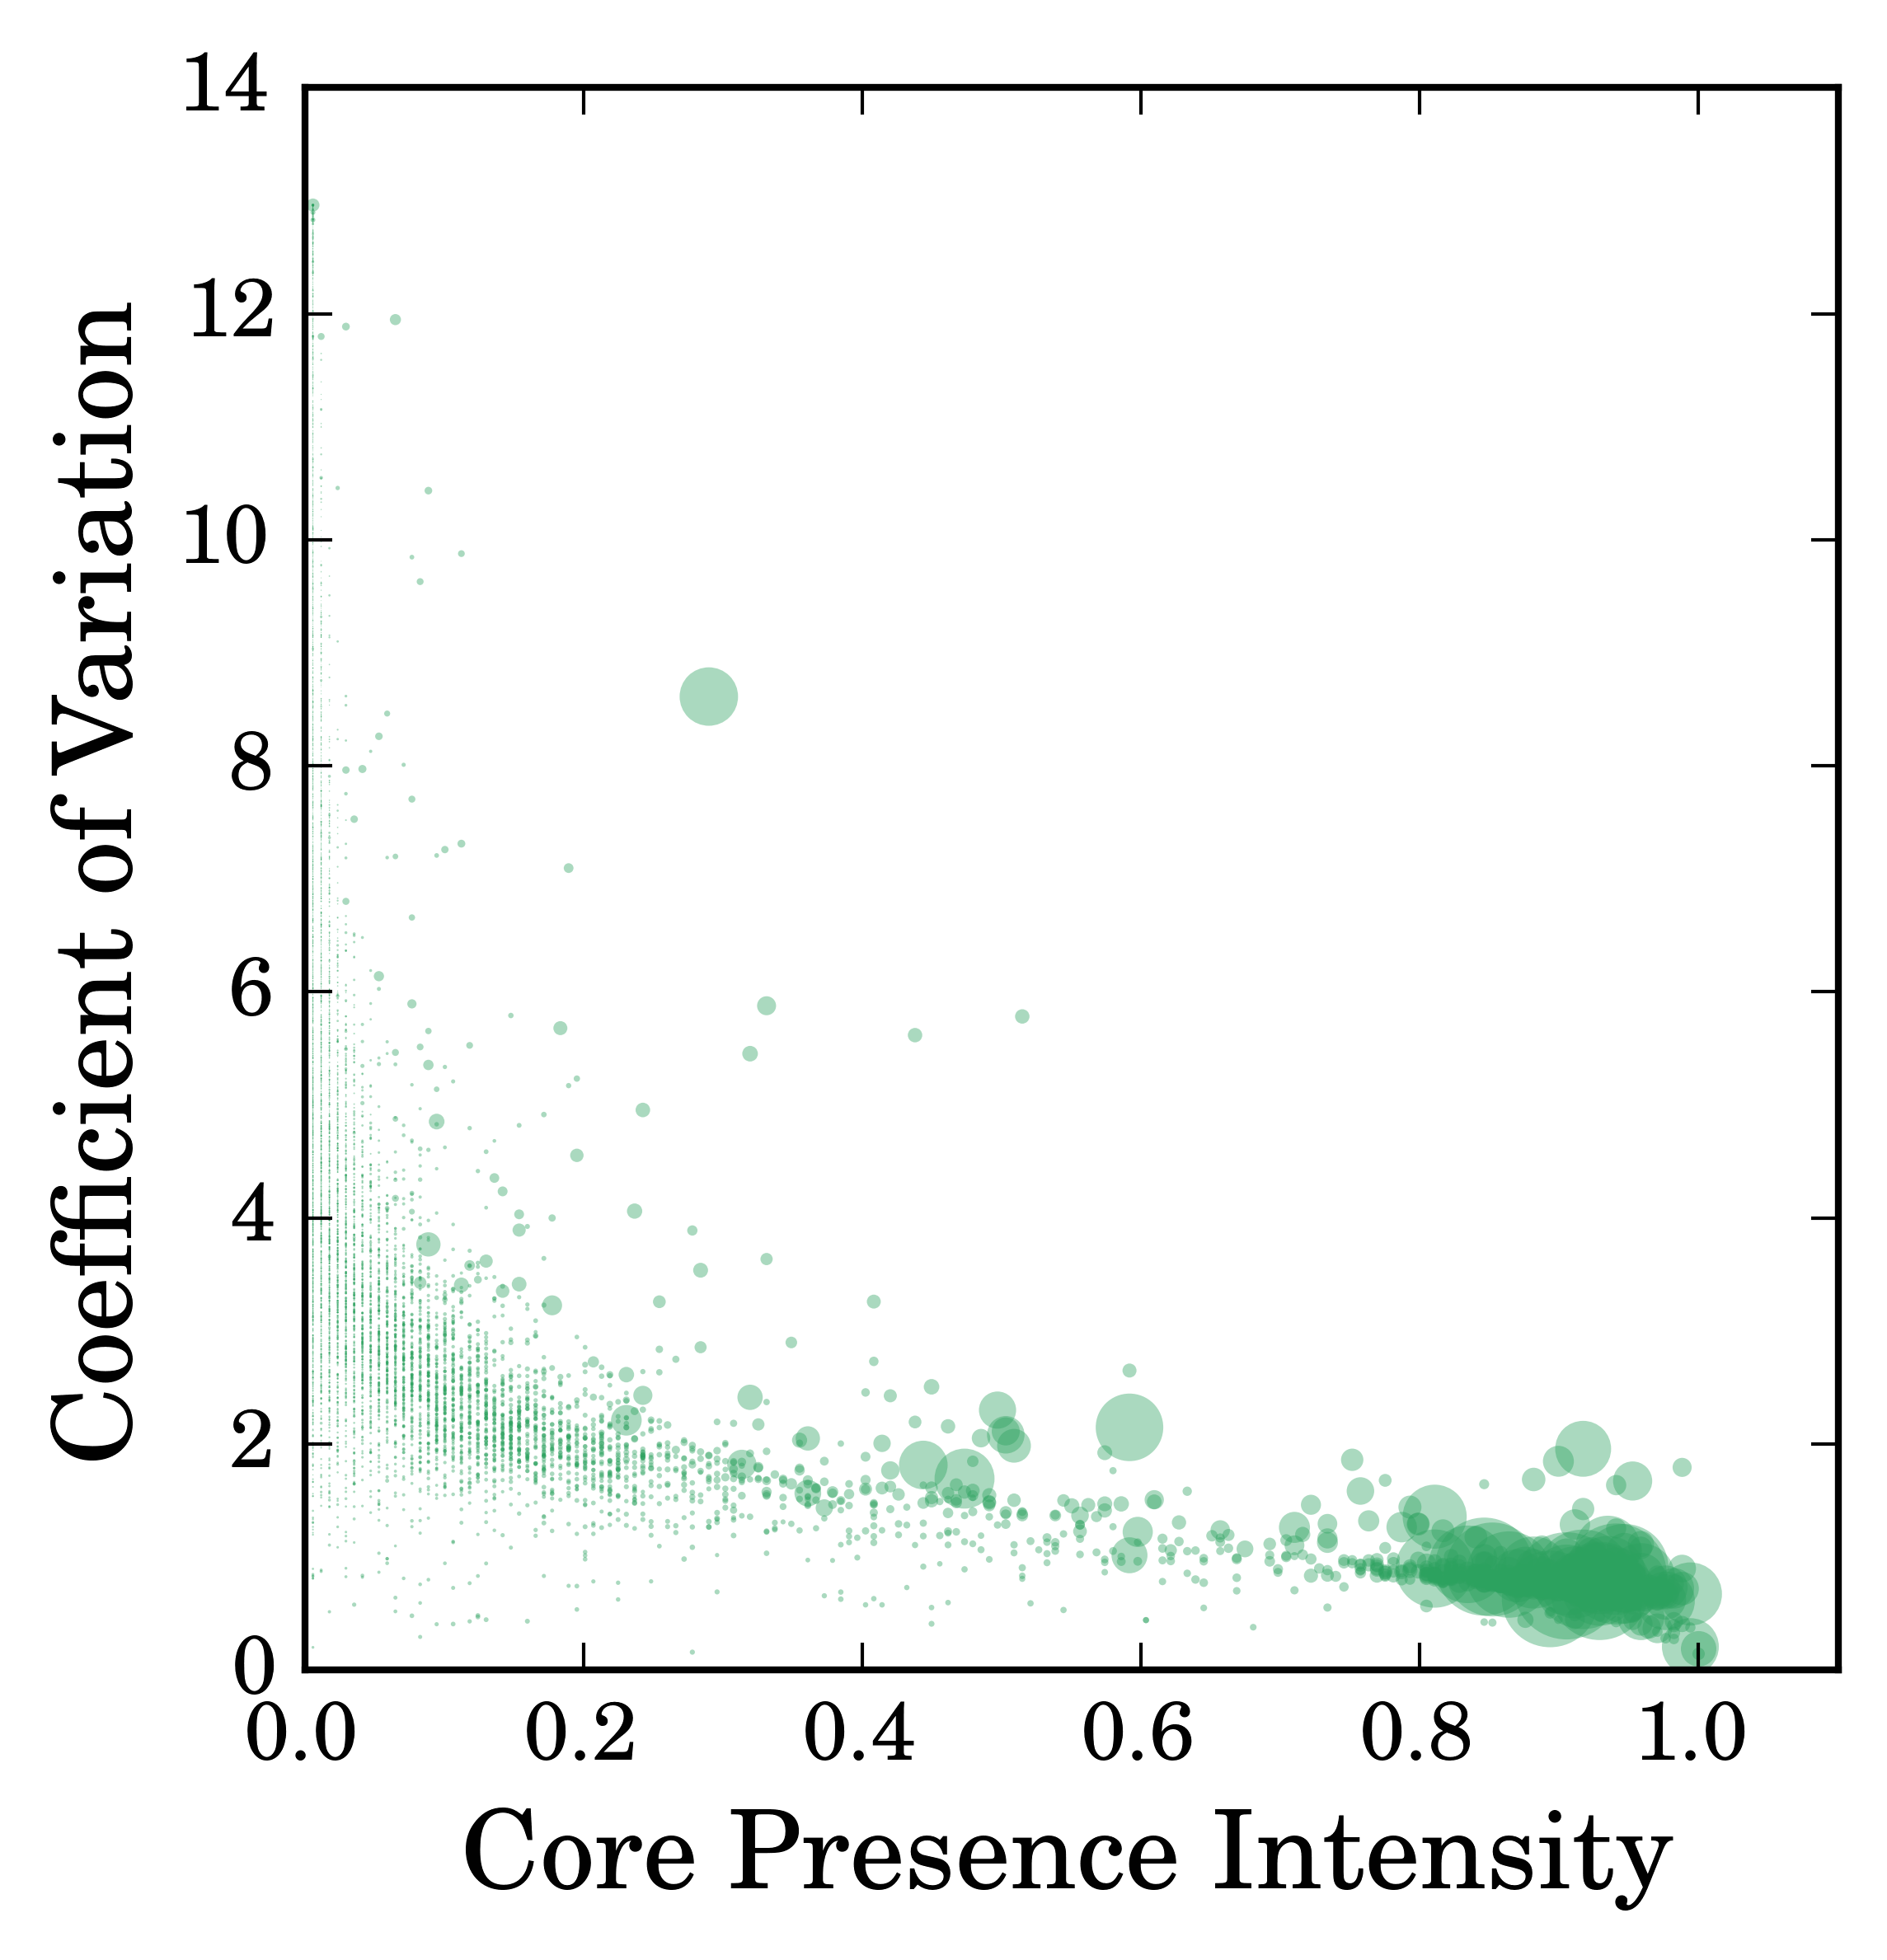
\includegraphics[width=\textwidth]{gfx/chap2/corre_cv_cp_sh.png}
                \caption{SH, 52061 prefixes}
                \label{fig:cv_cp_sh}
        \end{subfigure}
        \begin{subfigure}[b]{0.49\textwidth}
                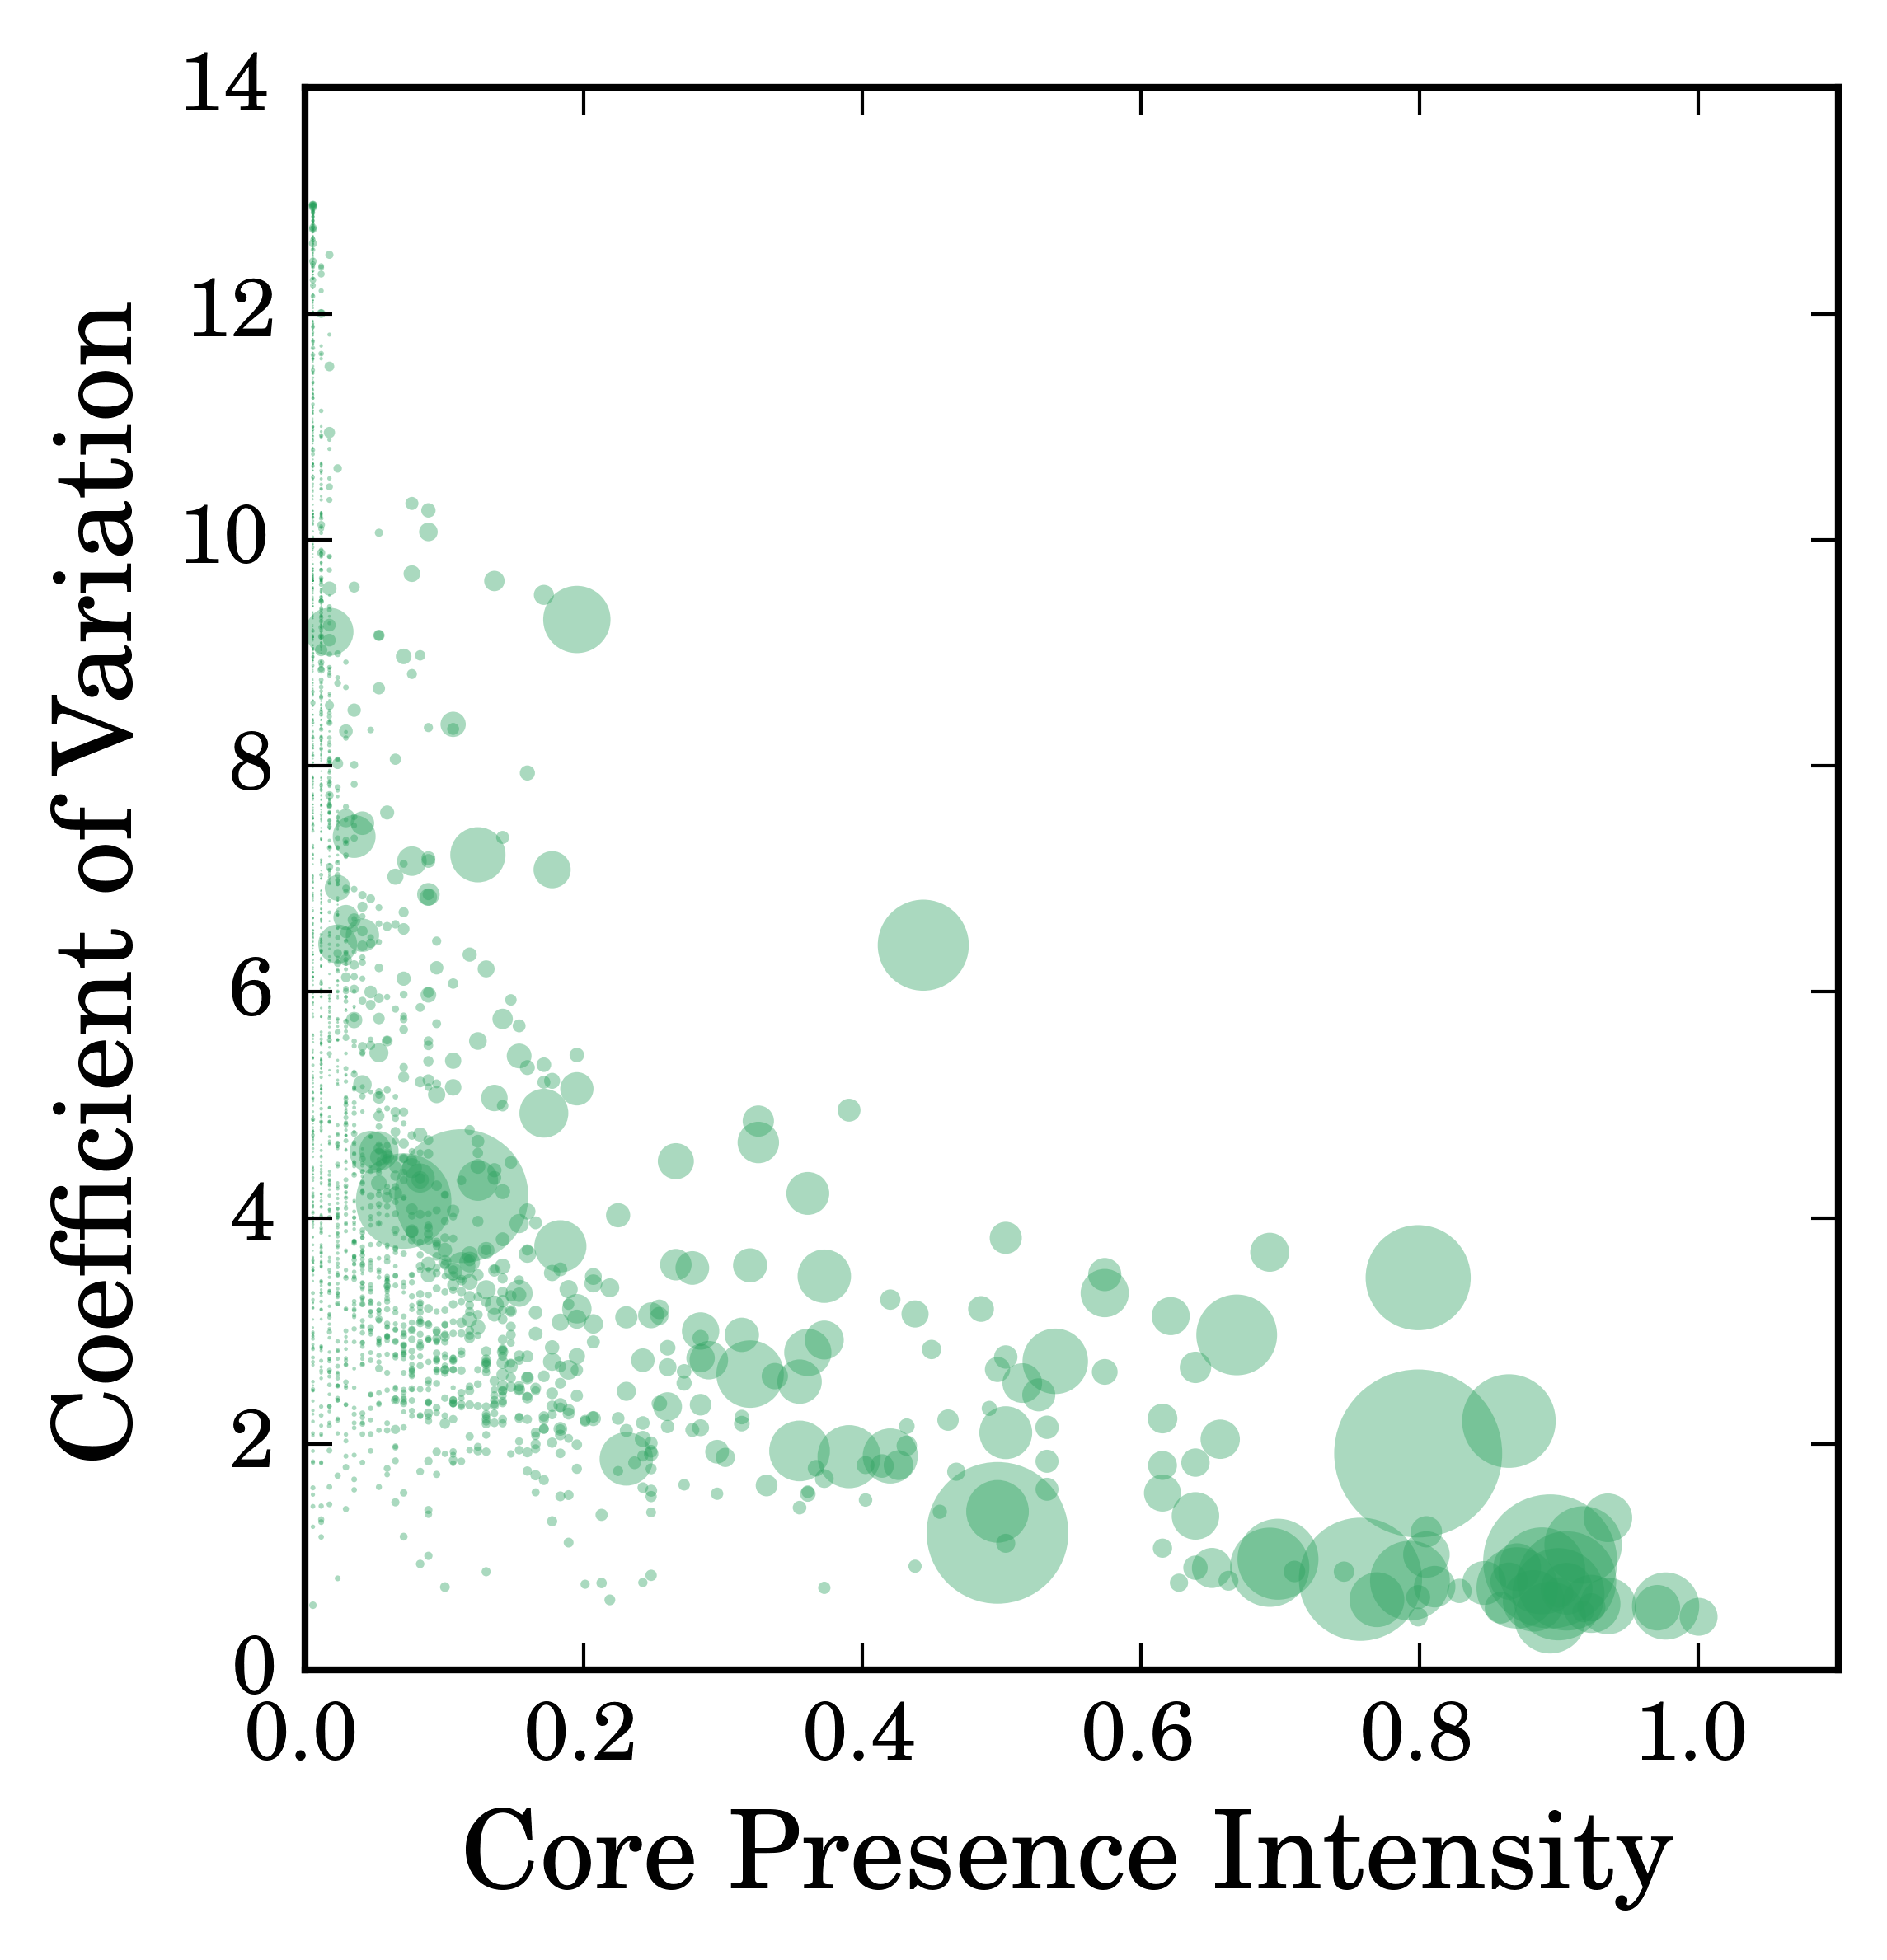
\includegraphics[width=\textwidth]{gfx/chap2/corre_cv_cp_si.png}
                \caption{SI, 14189 prefixes}
                \label{fig:cv_cp_si}
        \end{subfigure}
\caption{(cont.) Relation between $I_{cp}$ over one week and $c_v$ of hour volume over the week from June 1st, 2015.}
\label{fig:cv_cp_cont}
\end{figure}

It is interesting to study the correlation between these two metrics: $c_v$ %of hour volume throughout the week 
and $I_{cp}$ in Fig.~\ref{fig:cv_cp}, where each circle represents a prefix and its radius is proportional to the prefix's week volume share.
The biggest circles mostly concentrate in the lower right corner of each sub-graph, which corresponds to the remarks made previously.
However, some exceptions exist, especially on SC (but also SF, SG and SI), where we observe circles of big sizes having low $I_{cp}$ and relatively high $c_v$.
These prefixes bring significant traffic volume share within a short duration, which makes predictive prefix selection difficult. 
Finally, it's not a surprise to see that the $c_v$ of prefixes with big week volume is, to a certain extent, inversely correlated to their $I_{cp}$.
%That is, when a prefix is associated with larger week traffic volume, chances are it has smaller variation in hour volumes and presents more often in the \textit{core} set.

\subsubsection{A view at hour interval}
\begin{figure}
\centering
		\centering
        \begin{subfigure}[b]{0.85\textwidth}
                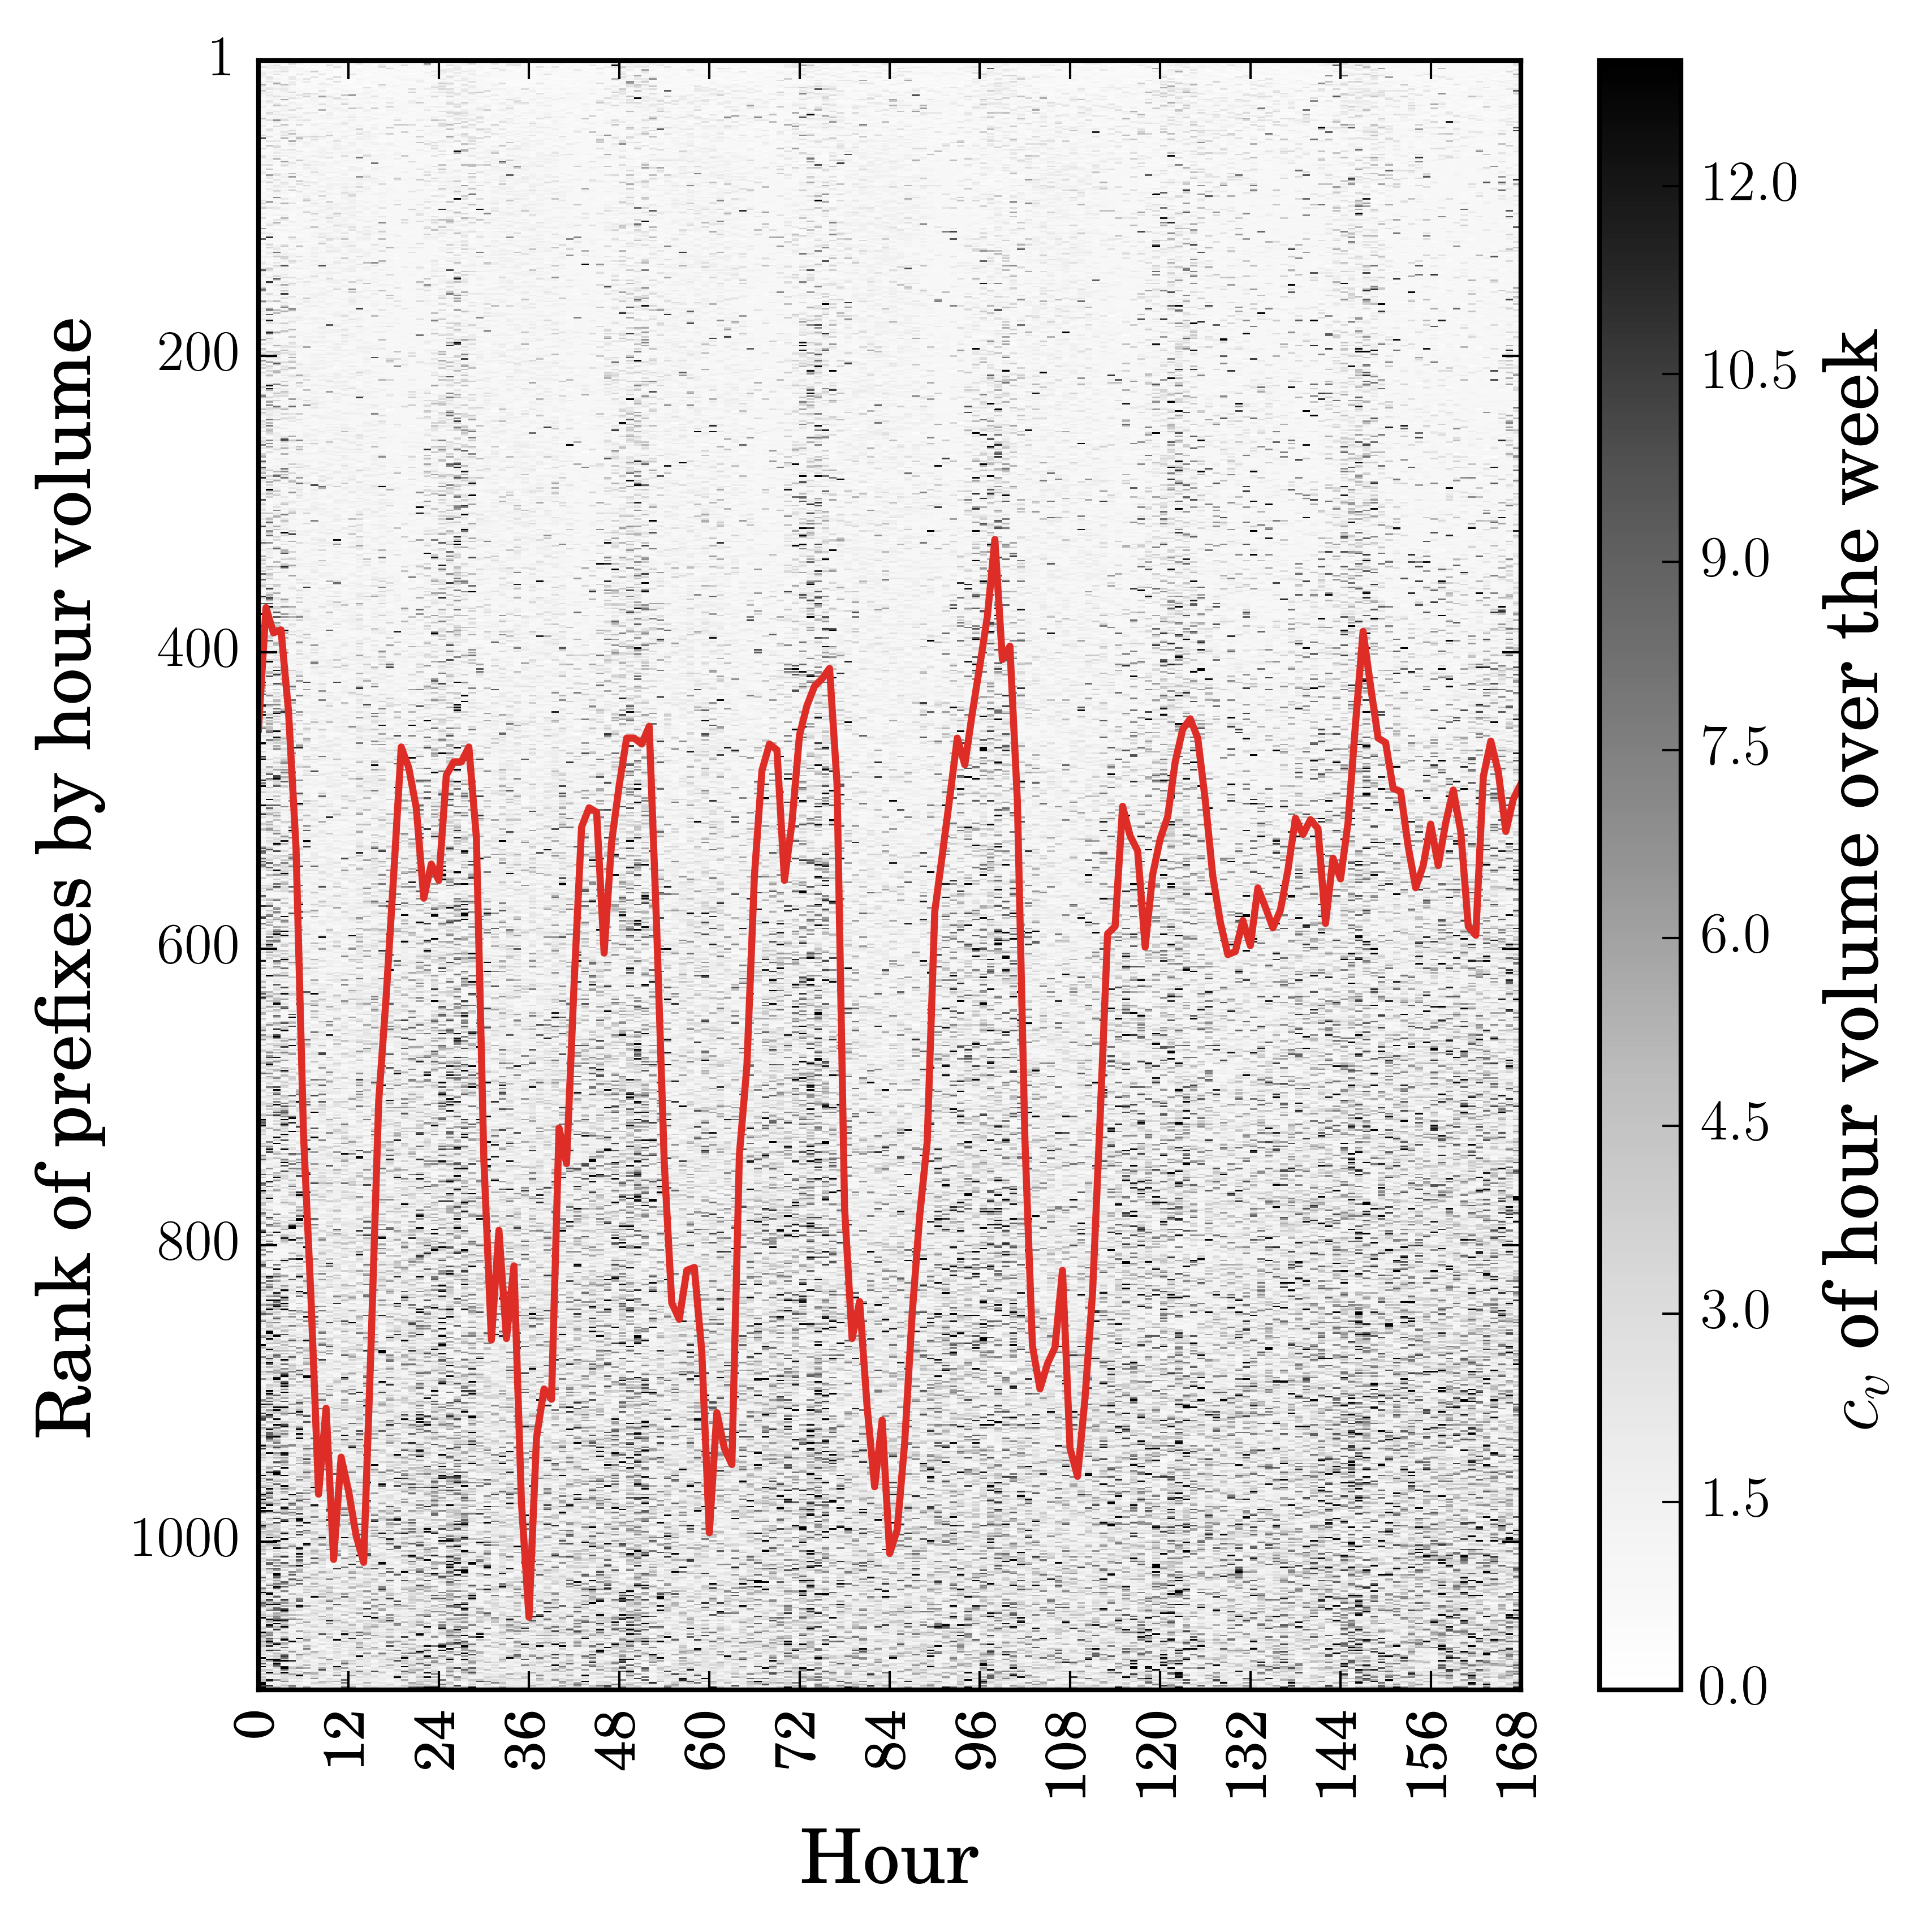
\includegraphics[width=\textwidth]{gfx/chap2/cv_mat_sa.png}
                \caption{$c_v$}
                \label{fig:cv_mat_sa}
        \end{subfigure}
        \begin{subfigure}[b]{0.85\textwidth}
                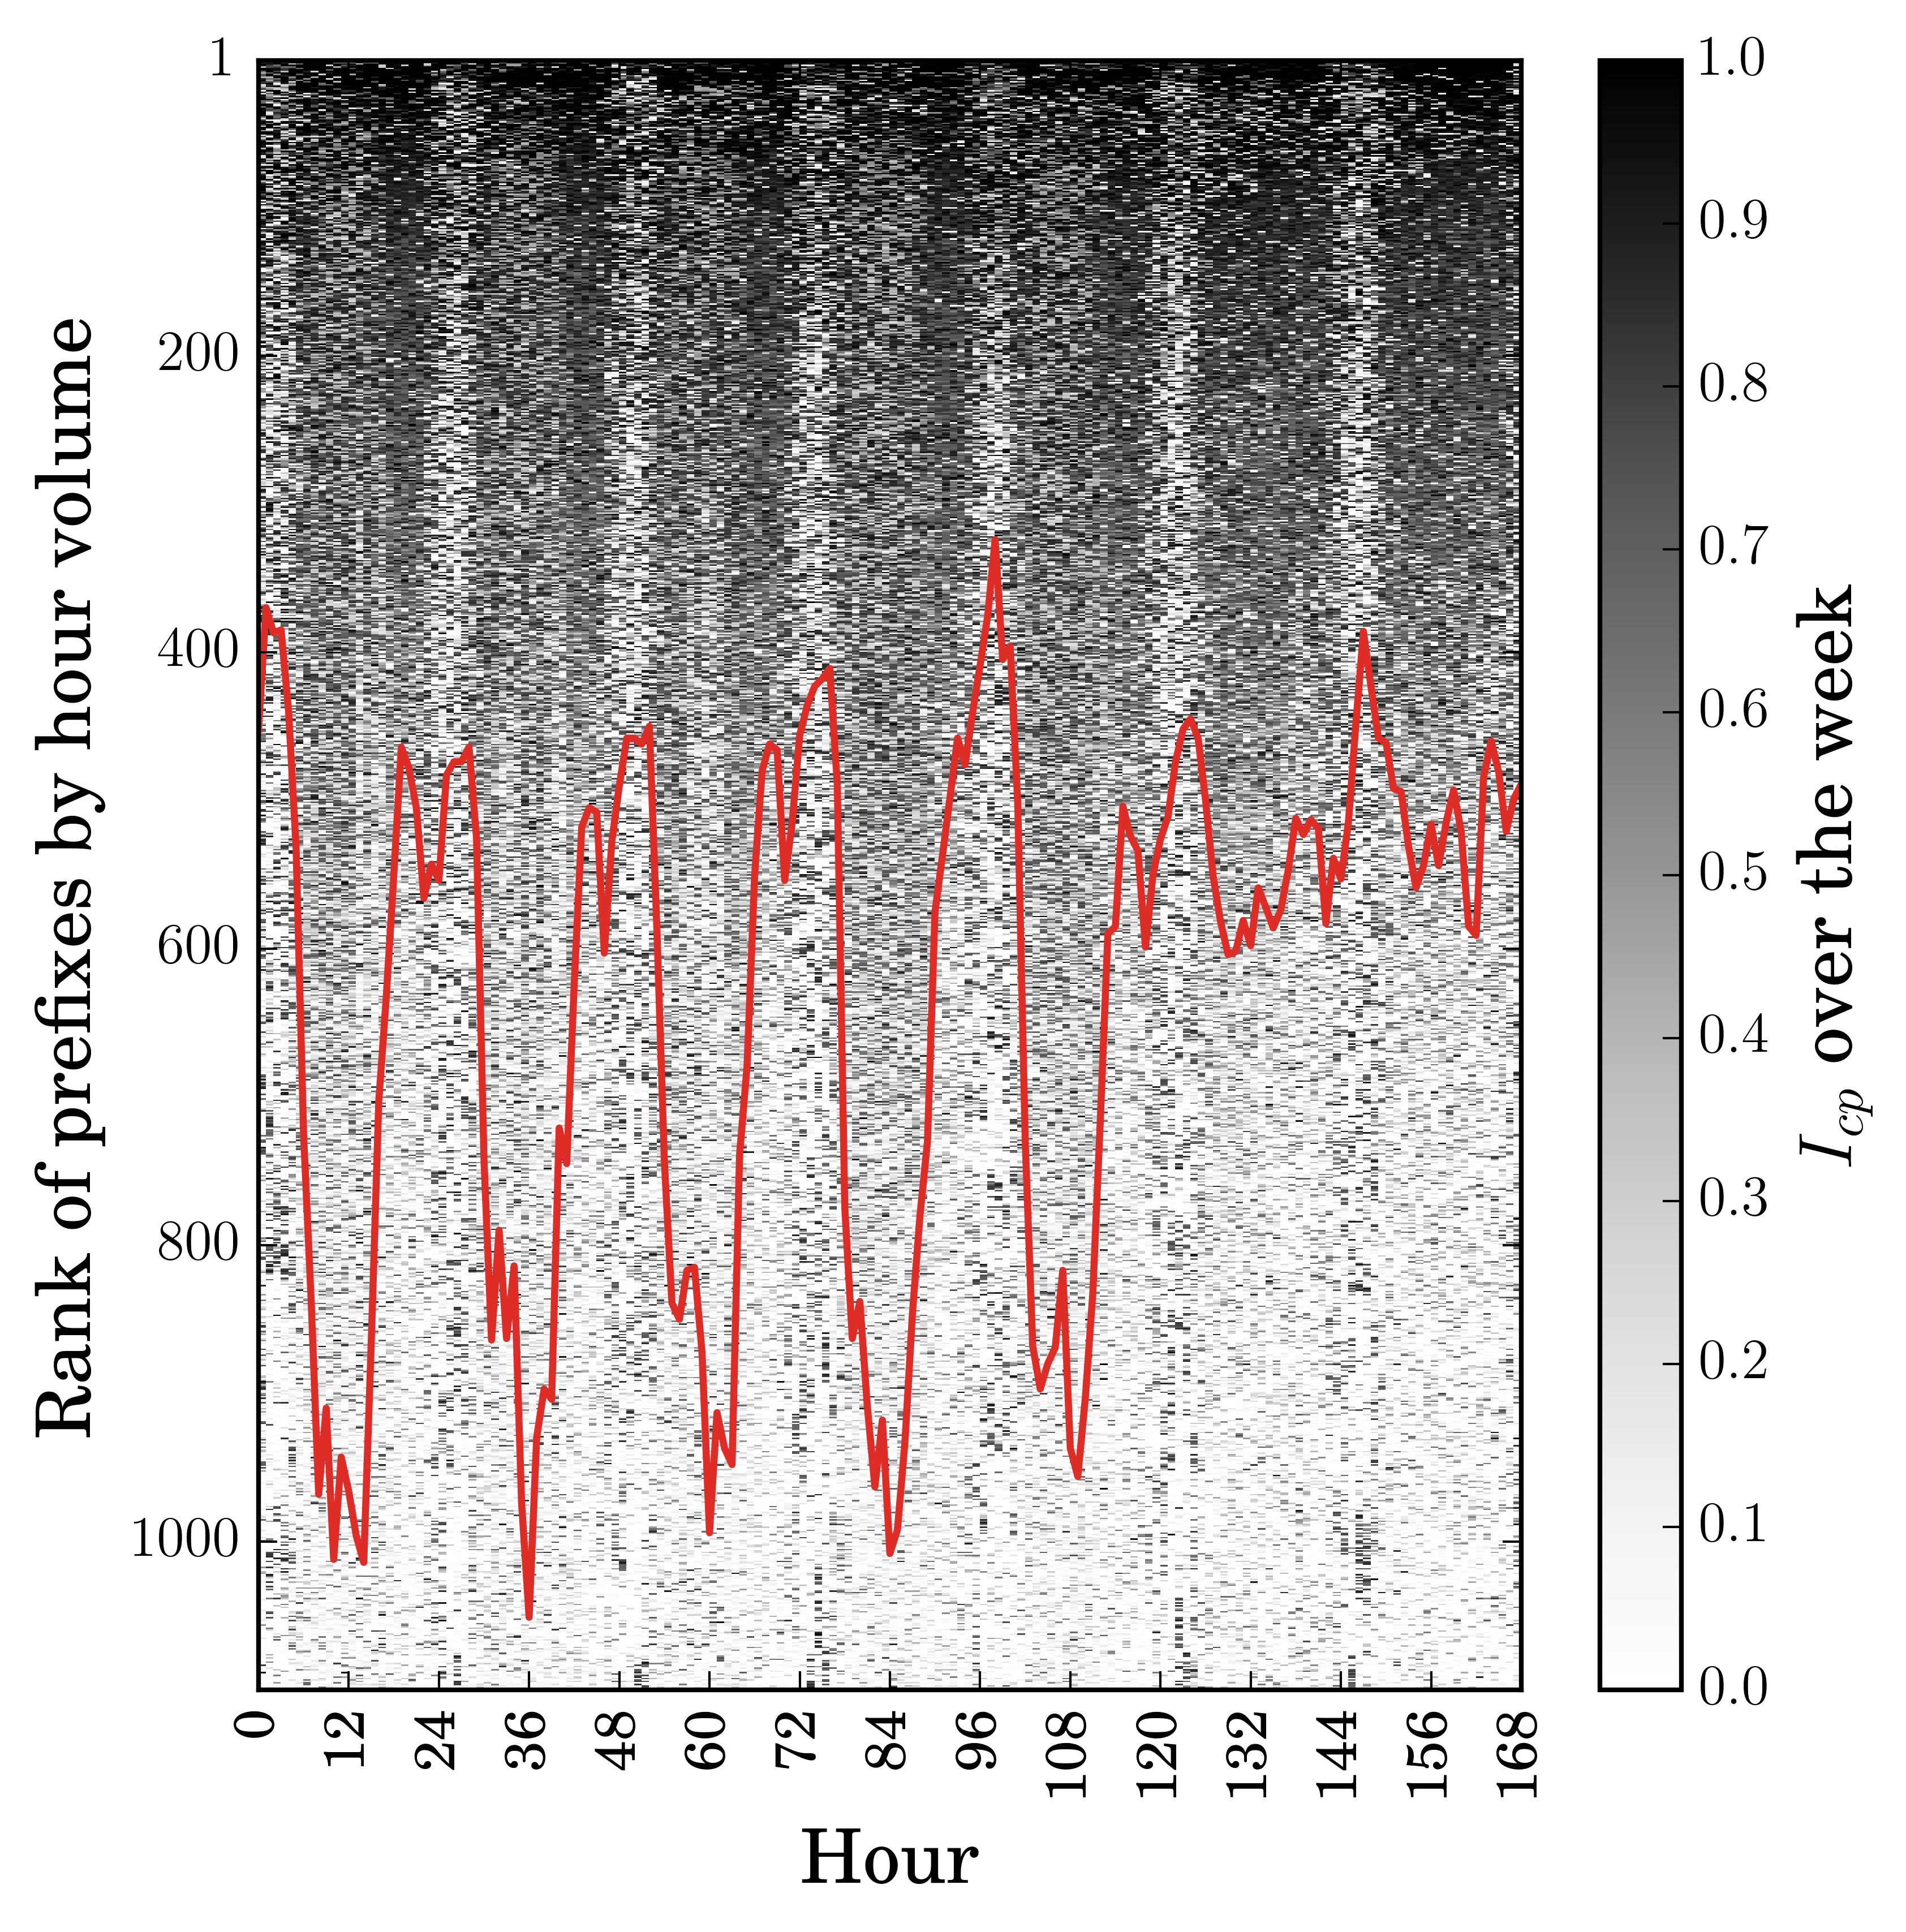
\includegraphics[width=\textwidth]{gfx/chap2/cp_mat_sa.png}
                \caption{$I_{cp}$}
                \label{fig:cp_mat_sa}
        \end{subfigure}
\caption{$c_v$ and $I_{cp}$ over one week for top ranked prefixes at each hour on SA. Prefixes are ranked by their hour volume along the column (big prefixes at the top). Their $c_v$ or $I_{cp}$ over the week are represented by the grey scale. Red line indicates the number of prefixes in \textit{core} prefix set each hour.}
\label{fig:cv_cp_mat}
\end{figure}

The above analyses at week scale conclude that most prefixes associated with a big volume over a long term tend to be stable in hour volume variation and present often in \textit{core}, though a few exceptions exist.
Here, we explore the prefix volume dynamism at hour resolution by visualizing them in Fig.~\ref{fig:cv_cp_mat}, where each column corresponds to top prefixes ranked by their hour volume with large volume prefixes at the top and small ones at the bottom. A grey scale tile is used to portrait the $c_v$ or $I_{cp}$ over the week for each prefix. Prefixes above the red line are those composing \textit{core} at each hour.
Only graphs for SA are shown for the patterns demonstrated are most informative and less noisy due to less bursty traffic.

In Fig.~\ref{fig:cv_mat_sa} the graph for $c_v$, area above the red line has observably lighter value than the lower part. 
This implies that in each hour, prefixes in the \textit{core} have more stable hour volume over a long term, i.e. closer to its mean value,  than those outsiders with little volume significance.
Moreover, the figure demonstrates as well a time-of-day pattern. 
During late night and early morning, prefixes in the \textit{core} have deeper color, thus more volatile, than those in the day time, which indicates that important prefixes composition are not quite the same over these two periods.

The above described phenomenon are sometimes a little bit more difficult to be perceived on other networks with more bursty traffic. 
Nonetheless, the color value for \textit{core} area is not visibly darker.
It means the hourly volume time series for large prefixes are not obviously more stable.
However, we should all the same be able to pick them out using their mean value.
The lack of clear diurnal pattern is possibly related to their business types and client populations they serve, which is out of the scope of this work.

When it comes to $I_{cp}$, it is true for all networks that top ranked prefixes each hour are more likely to frequently appear in the \textit{core} prefix set, which leads to deeper color at the top.
However, we can witness light spots each hour in the upper part of the graph, which corresponds to bursty traffic.
Further, the color difference across the red line is not obvious.
This indicates $I_{cp}$ alone is not informative enough to tell whether a prefix brings a big amount of traffic at a certain hour, though for long term it demonstrate strong correlation with volume importance as seen in Fig.~\ref{fig:cpi}.
Time-of-day pattern can also be clearly observed. It confirms again that prefixes active over night are different from those during day time.


\subsection{Quantitative index of traffic burstiness}
Previous explorations has shown that the predictability of traffic volume from a client network is related to its traffic burstiness.
In order to describe traffic burstiness in a quantitative manner, we define the index $\beta(P)_h$, for a prefix $P$ at certain hour $h$ as:
\begin{equation*}
\beta(P)_i = \begin{dcases*}
         -\log(I_{cp}(P)) \times vp(P)_i & if $I_{cp}(P) > 0$\\
        0 & if $I_{cp}(P) = 0$,
        \end{dcases*}
\label{eq:beta}
\end{equation*}
where $vp(P)_h$ is the hour volume percentage (among all active prefixes) of prefix $P$ at hour $h$.
The logarithmic term applied on $I_{cp}$ aims at amplifying the volume contribution of prefixes with rare \textit{core} presence, and attenuating the influence of prefixes being intensively in the \textit{core}.
A large $\beta$ value indicates that it is hard to predict the volume associated with this prefix while representing a significant hour volume.

In order to estimate the overall impact brought by bursty traffic at hour $h$ for a client network, we sum up the $\beta(P)_h$ for each $P$ inside the \textit{core} of that hour: more formally, 
%Wenqin: notation for $\beta(P)_i$ is not right
\begin{equation*}
BI_h = \sum_{P \in \textit{core}_h} \beta(P)_h.
\label{eq:bi}
\end{equation*}
%Wenqin: notation for $\beta(P)_i$ is not right
For all the networks, we estimate their traffic burstiness with the mean and maximum value of $BI$ series over the week. The results are given in Table~\ref{tab:bi}. The maximum $\beta$ over all the week is also given for the sake of clarity.
\begin{table}[!tb]
\centering
\begin{tabular}{cccc}\toprule
\textbf{Network} & \textbf{Mean $BI$} & \textbf{Max $BI$} & \textbf{Max $\beta$}\\
\midrule
SA & 14.61 & 37.79  &  7.44\\
SB & 31.09 & 46.85  &  4.08\\
SC & 40.57 & 145.07 &  145.05\\
SD & 42.14 & 69.34  &  18.10\\
SE & 20.91 & 44.30  &  20.17\\
SF & 44.10 & 98.69  &  78.77\\
SG & 51.21 & 125.41 &  102.05\\
SH & 15.91 & 35.06  &  16.29\\
SI & 38.59 & 85.47  &  56.56\\
\bottomrule
\end{tabular}
\caption{Traffic burstiness.}
\label{tab:bi}
\end{table}

Mean $BI$ over the week measures the overall impact brought by bursty traffic, while maximum $BI$ describes the degree of burstiness in worst cases.
In correspondence to the observation made from Fig.~\ref{fig:cv_cp}, there are big volume prefixes with fairly low $I_{cp}$ on SC, SF, SG and SI, whence the much bigger maximum $\beta$ value.
What is less evident in Fig.~\ref{fig:cv_cp} is that SD suffers actually a lot from bursty traffic, even more than SC in general.
For the rest networks, i.e. SA, SB, SE and SH, their mean $BI$ over the week is around 30 or lower. Their corresponding sub-graphs in Fig.~\ref{fig:cv_cp} manifest as well much less big circles on the left side where $I_{cp}$ is low.
More specifically SB suffers more from bursty traffic than SA, therefore bigger value in both maximum and mean $BI$ over the week, which is as well not easy to tell directly from Fig.~\ref{fig:cv_cp}.
%which is in accordance with the observation that the tone of \textit{core} area of SB is lighter than that of SA in Fig~\ref{fig:cp_mat}.
Still, the maximum $\beta$ on SA is larger than that on SB, which is due to the fact that traffic on SB is more evenly distributed among active prefixes (see Fig.~\ref{fig:traffic_dis_site}), and the faction of traffic associated to each prefix is generally smaller.
In short, we found this simple metric capable of describing the traffic burstiness of the networks studied.




\section{Predictive prefix selection}
\label{sec:sele}


\subsection{Candidate prediction metrics}

\marginpar{prediction metrics inspired by traffic temporal dynamism studies}
Based on the previous observations, several approaches naturally emerges for the prediction of traffic volume ``importance'' of a prefix.

\paragraph*{Mean Volume}
With this metric, we predict that at hour $h+1$, the volume importance of prefix $P$ is indicated by it's mean hourly volume over the last $L$ hours, $MV(P,L)_{h+1} = 1/L \times \sum_{i = h-L+1}^{h} v(P)_i$.
It is based on the observations from Fig.~\ref{fig:cv}, that top prefixes ranked over the week tend to have smaller hourly volume variation around their mean volume.

\paragraph*{Core Presence Intensity}
The prediction could use $I_{cp}(P,L)_{h+1} = 1/L \times \sum_{i = h-L+1}^{h} cp(P)_i$, i.e. the \textit{core} presence intensity of the prefix over the last $L$ hours. It derives from the observation made from Fig.~\ref{fig:cpi}, that high ranked prefixes by their week volume are more likely to have intense \textit{core} presence.

\paragraph*{Core Volume}
Finally, the prediction could be based on $CV(P,L)_{h+1} = 1/L \times \sum_{i = h-L+1}^{h} cp(P)_i \times v(P)_i$,  a combination of both $MV$ and $I_{cp}$.
$CV$ has the potential to be more resource thrifty compared to $MV$, as it is calculated only for those prefixes ever appeared in the \textit{core} over the last $L$ hours --- while $MV$ is computed for all active prefixes. From our observations, the \textit{core} size actually represents $5\%$ to $50\%$ of all active prefixes.

\subsection{Grey model as reference method}
In previous work by Zhange et al.\ \cite{Zhang2012} on FIB caching, a grey differential model $GM(1,1)$ \cite{Julong1989} is employed to  predict which BGP prefixes will represent the  biggest packet counts. 
It is by far the more computationally efficient ($O(L)$), compared to \ac{TSF} methos such as \ac{ANN} ($O(L*M)$) and \ac{ARIMA} ($O(L^2)$), where L is the length of time series, M is the number of hidden nodes in the neural network.
For the sake of comparison, we implemented the $GM(1,1)$ model as well in our work. 

A brief introduction to this model and how we apply it in our context is given below. Mathematical details of this model can be find in the work by Deng \cite{Julong1989}.

$GM(1,1)$ predicts the cumulative hour volume $v^1$ instead of hour volume directly:
\begin{equation*}
v^1(P,L)_{i} = \displaystyle \sum_{j=i-L+1}^{i} v(P)_j,
\end{equation*}
where $v^1(P,L)_{i}$ is the cumulative hour volume of prefix $P$ over last $L$ hours at hour $i$. The purpose is to derive $v(P)_{i+1}$, i.e. the volume in the following hour, from estimations of cumulative volumes of hour $i+1$ and $i$:
\begin{equation*}
\hat{v}(P)_{i+1} = \hat{v}^1(P,L)_{i+1} - \hat{v}^1(P,L)_{i},
\end{equation*}
where $\hat v$ and $\hat v ^1$ are all estimation values given by the model.
$GM(1,1)$ predicts that the cumulative hour volume at hour $i+1$ equals:
\begin{equation*}
\hat v ^1 (P,L)_{i+1} = (v(P)_{i-L+1} - \frac{b}{a}) e^{-aL} + \frac{b}{a},
\end{equation*}
where $a$ and $b$ are parameters that can be estimated with least square method (symbol with hat are all estimations).
\begin{equation*}
\mathbf{\hat a} = \begin{bmatrix}
\hat a \\ \hat b
\end{bmatrix} = \mathbf{(B^TB)^{-1}B^T Y},
\end{equation*}
where
\begin{equation*}
\mathbf{B} = \begin{bmatrix}
-0.5(v^1(P,L)_{i-L+2} + v^1(P,L)_{i-L+1}) & 1\\
-0.5(v^1(P,L)_{i-L+3} + v^1(P,L)_{i-L+2}) & 1\\
\cdots & \cdots \\
-0.5(v^1(P,L)_i + v^1(P,L)_{i-1}) & 1
\end{bmatrix},
\end{equation*}
\begin{equation*}
\mathbf{Y} = \begin{bmatrix}
v(P)_{i-L+2}\\
v(P)_{i-L+3}\\
\cdots\\
v(P)_i
\end{bmatrix}.
\end{equation*}
We can see that for each single prefix, two parameters are to be estimated, $a$ and $b$, at each hour based on a new volume series that slides over time. Computationally, estimation with $GM(1,1)$ is much heavier than the three metrics proposed above, the calculation of which is identically to all prefixes without parameters to be customize.

\subsection{Prefix selection evaluation}
\begin{figure}
		\centering
        \begin{subfigure}[b]{0.48\textwidth}
                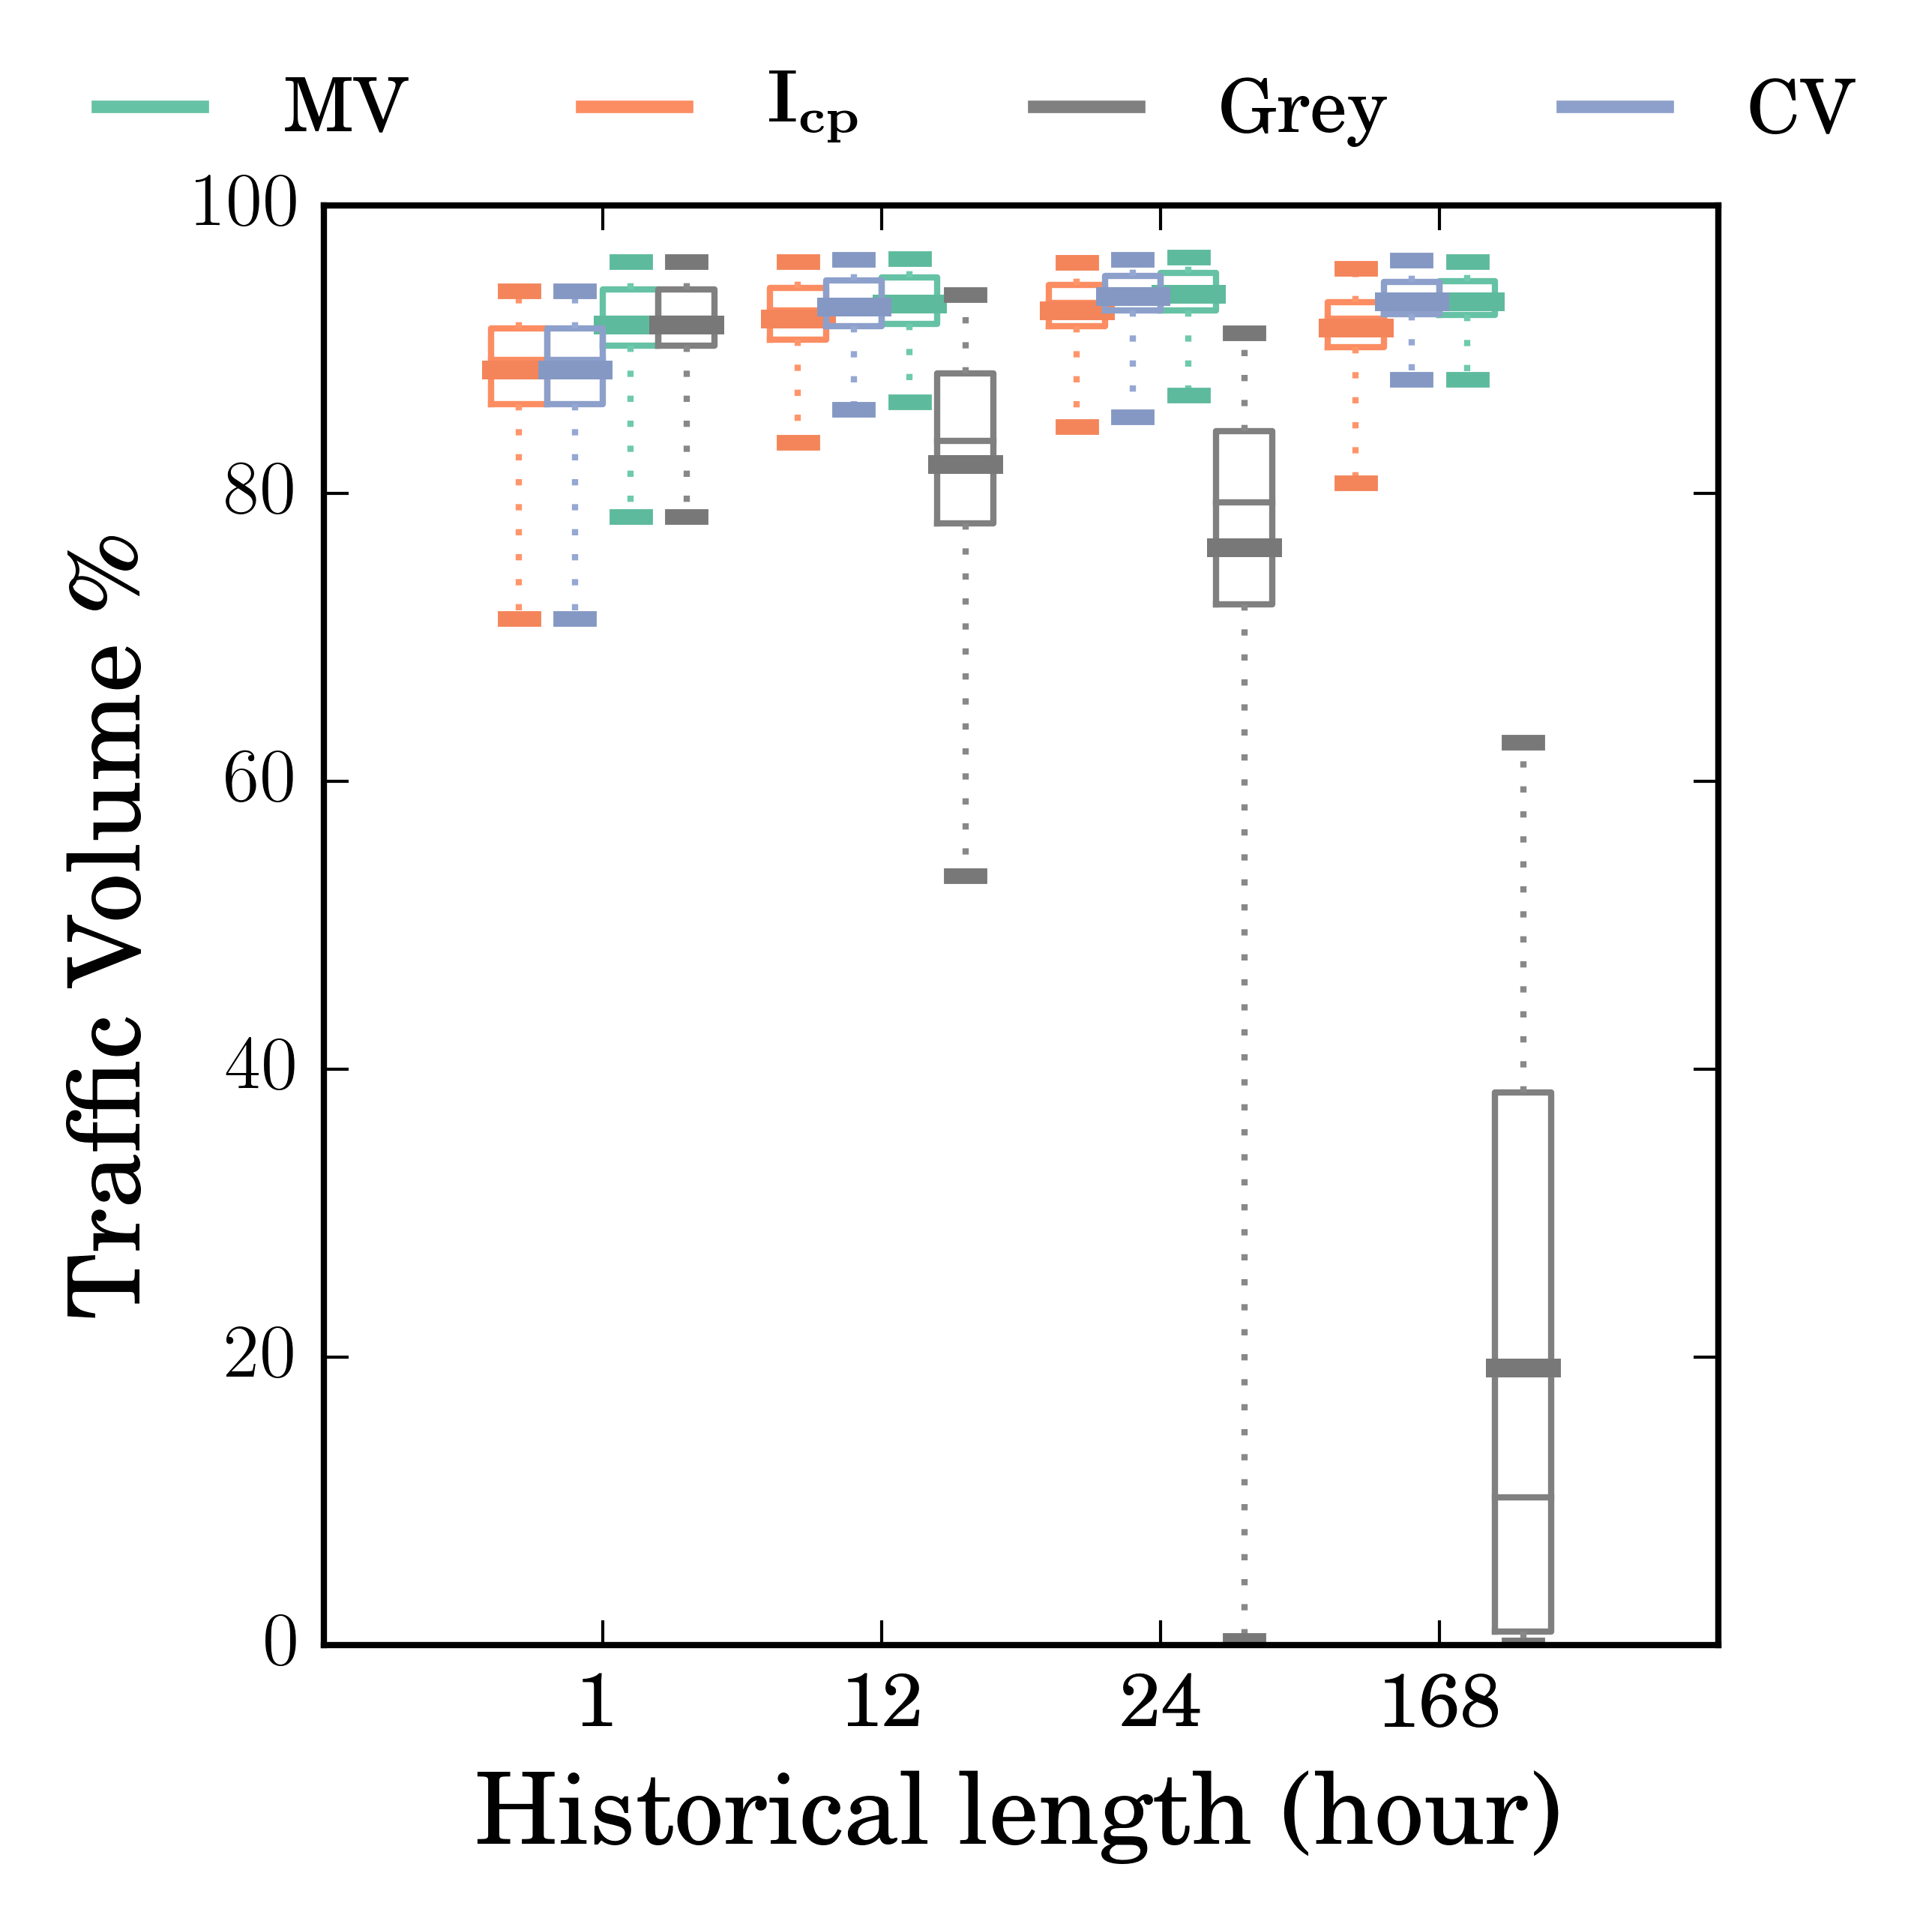
\includegraphics[width=\textwidth]{gfx/chap2/grey_cvg_box_method_compare_fs_sa.png}
                \caption{SA}
                \label{fig:cvg_sa}
        \end{subfigure}
        \begin{subfigure}[b]{0.48\textwidth}
                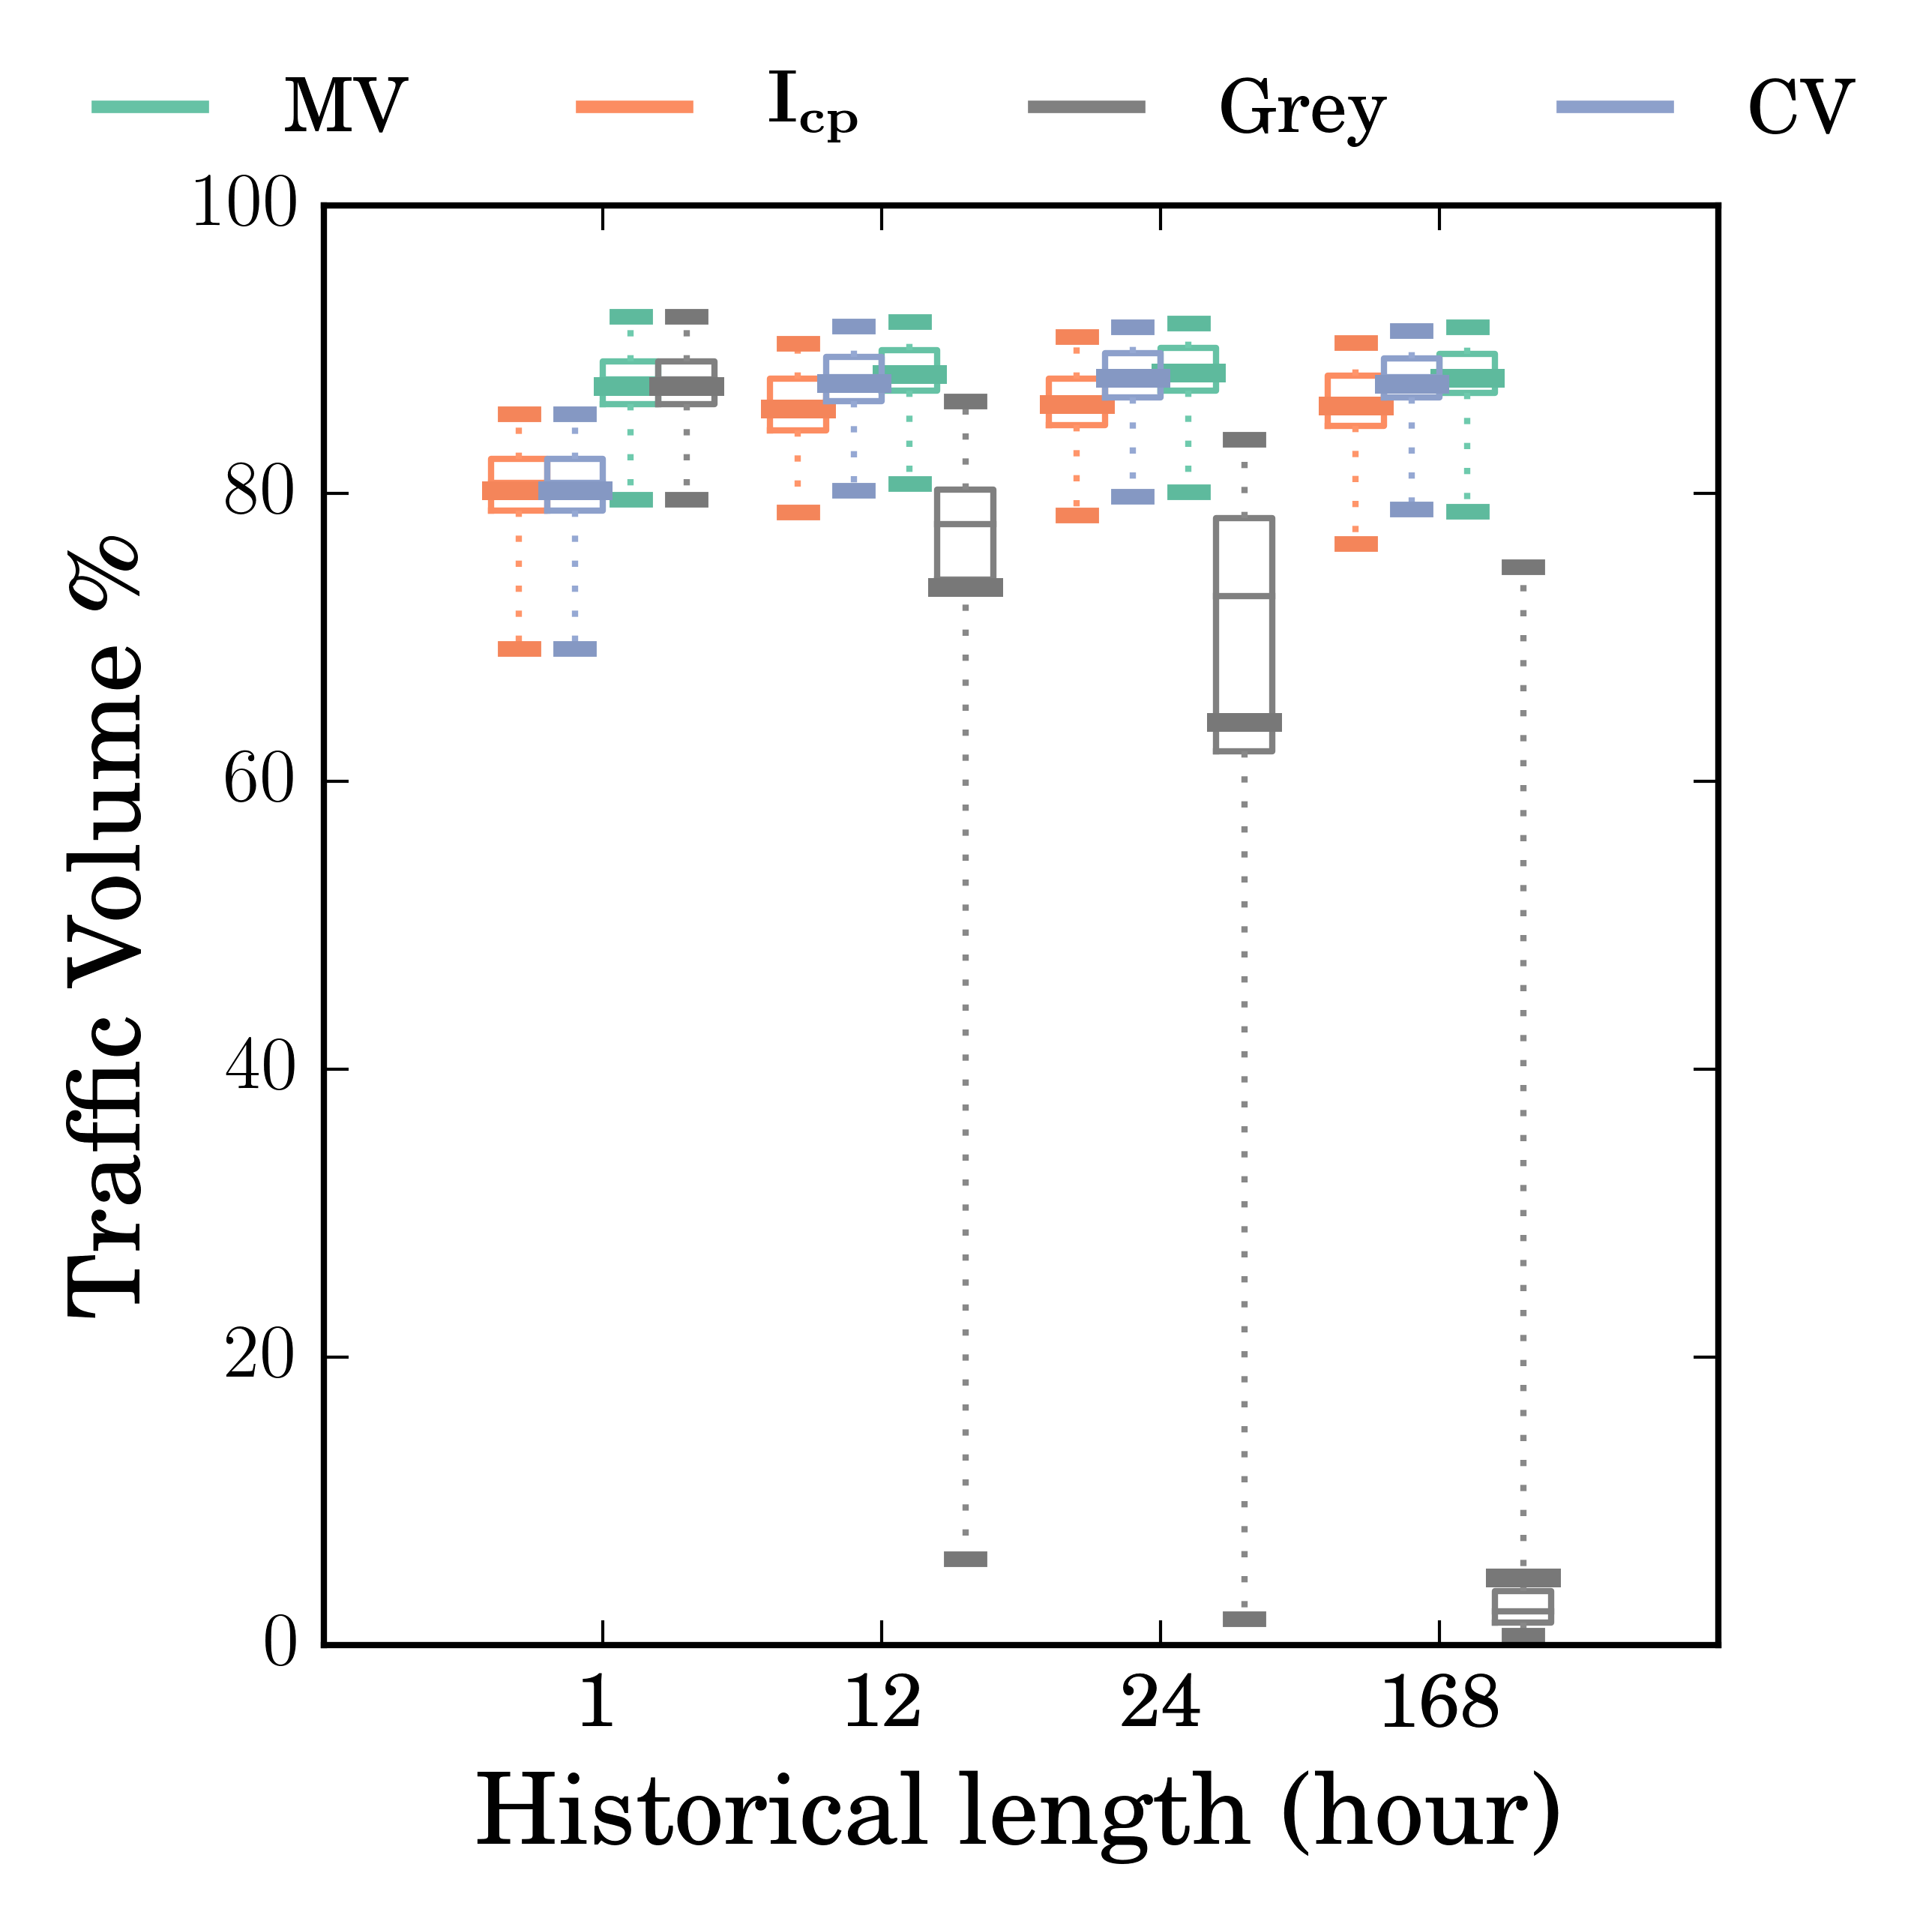
\includegraphics[width=\textwidth]{gfx/chap2/grey_cvg_box_method_compare_fs_sb.png}
                \caption{SB}
                \label{fig:cvg_sb}
        \end{subfigure}
        \begin{subfigure}[b]{0.48\textwidth}
                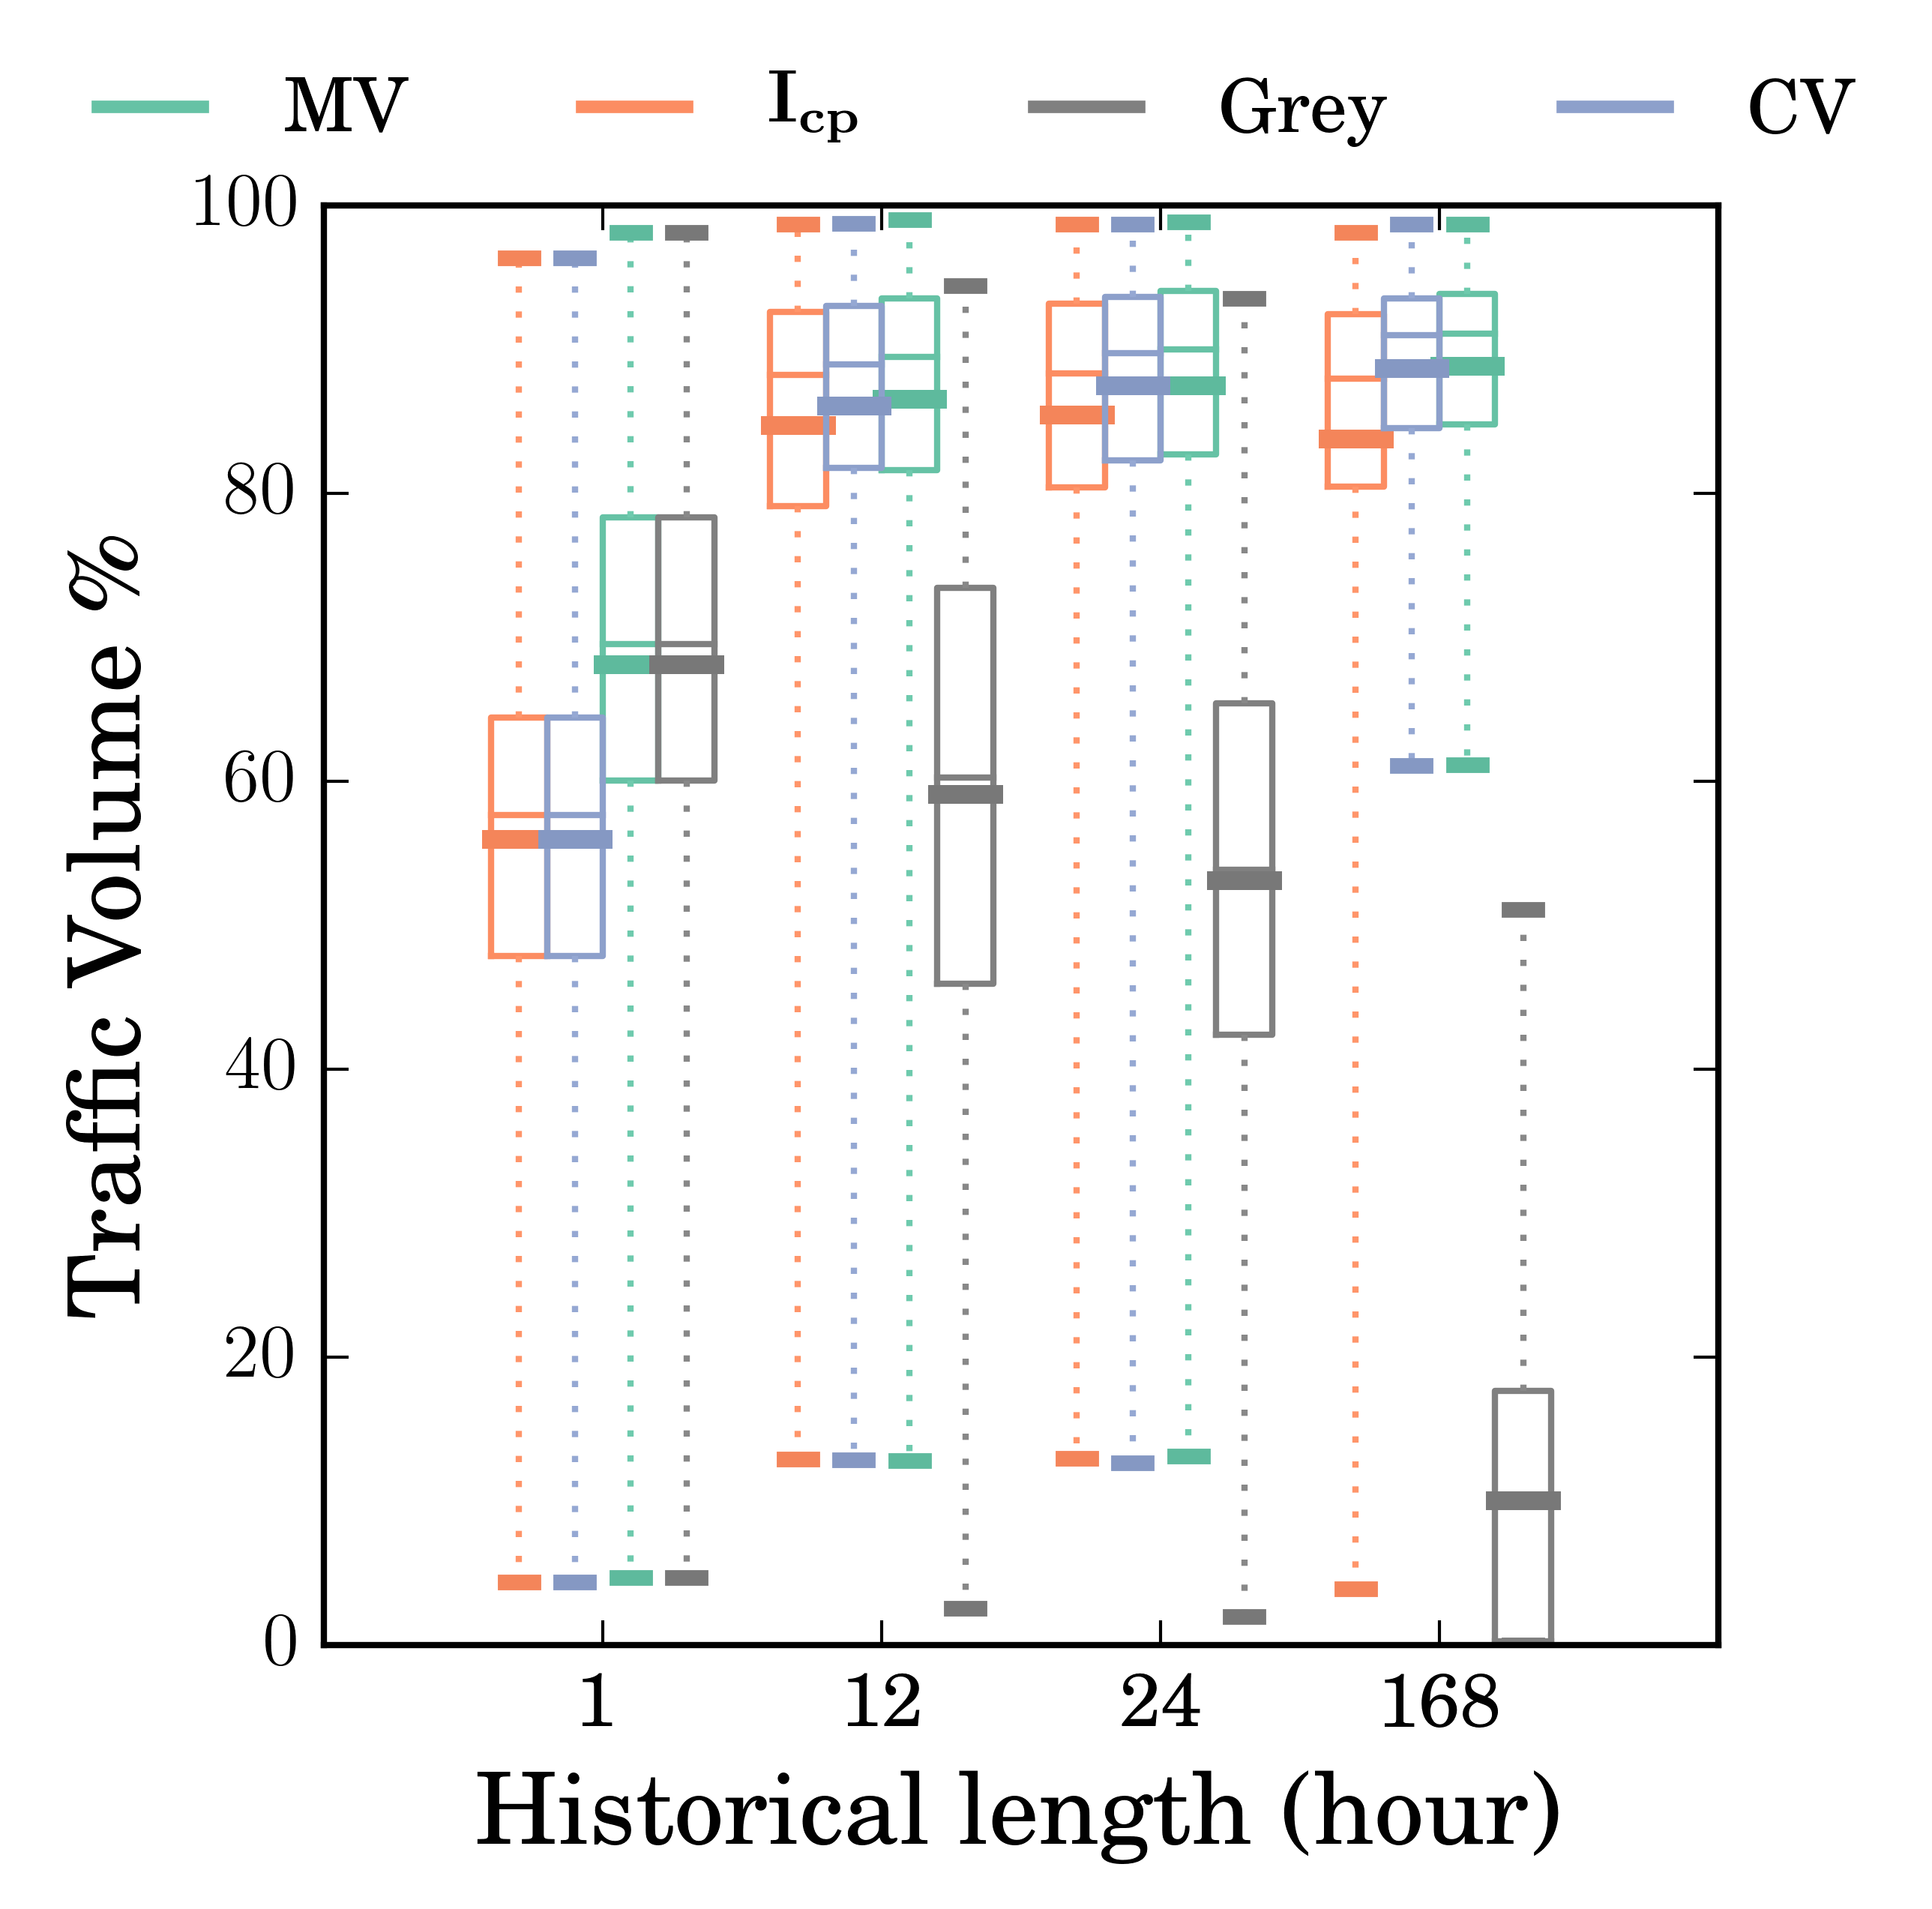
\includegraphics[width=\textwidth]{gfx/chap2/grey_cvg_box_method_compare_fs_sc.png}
                \caption{SC}
                \label{fig:cvg_sc}
        \end{subfigure}
        \begin{subfigure}[b]{0.48\textwidth}
                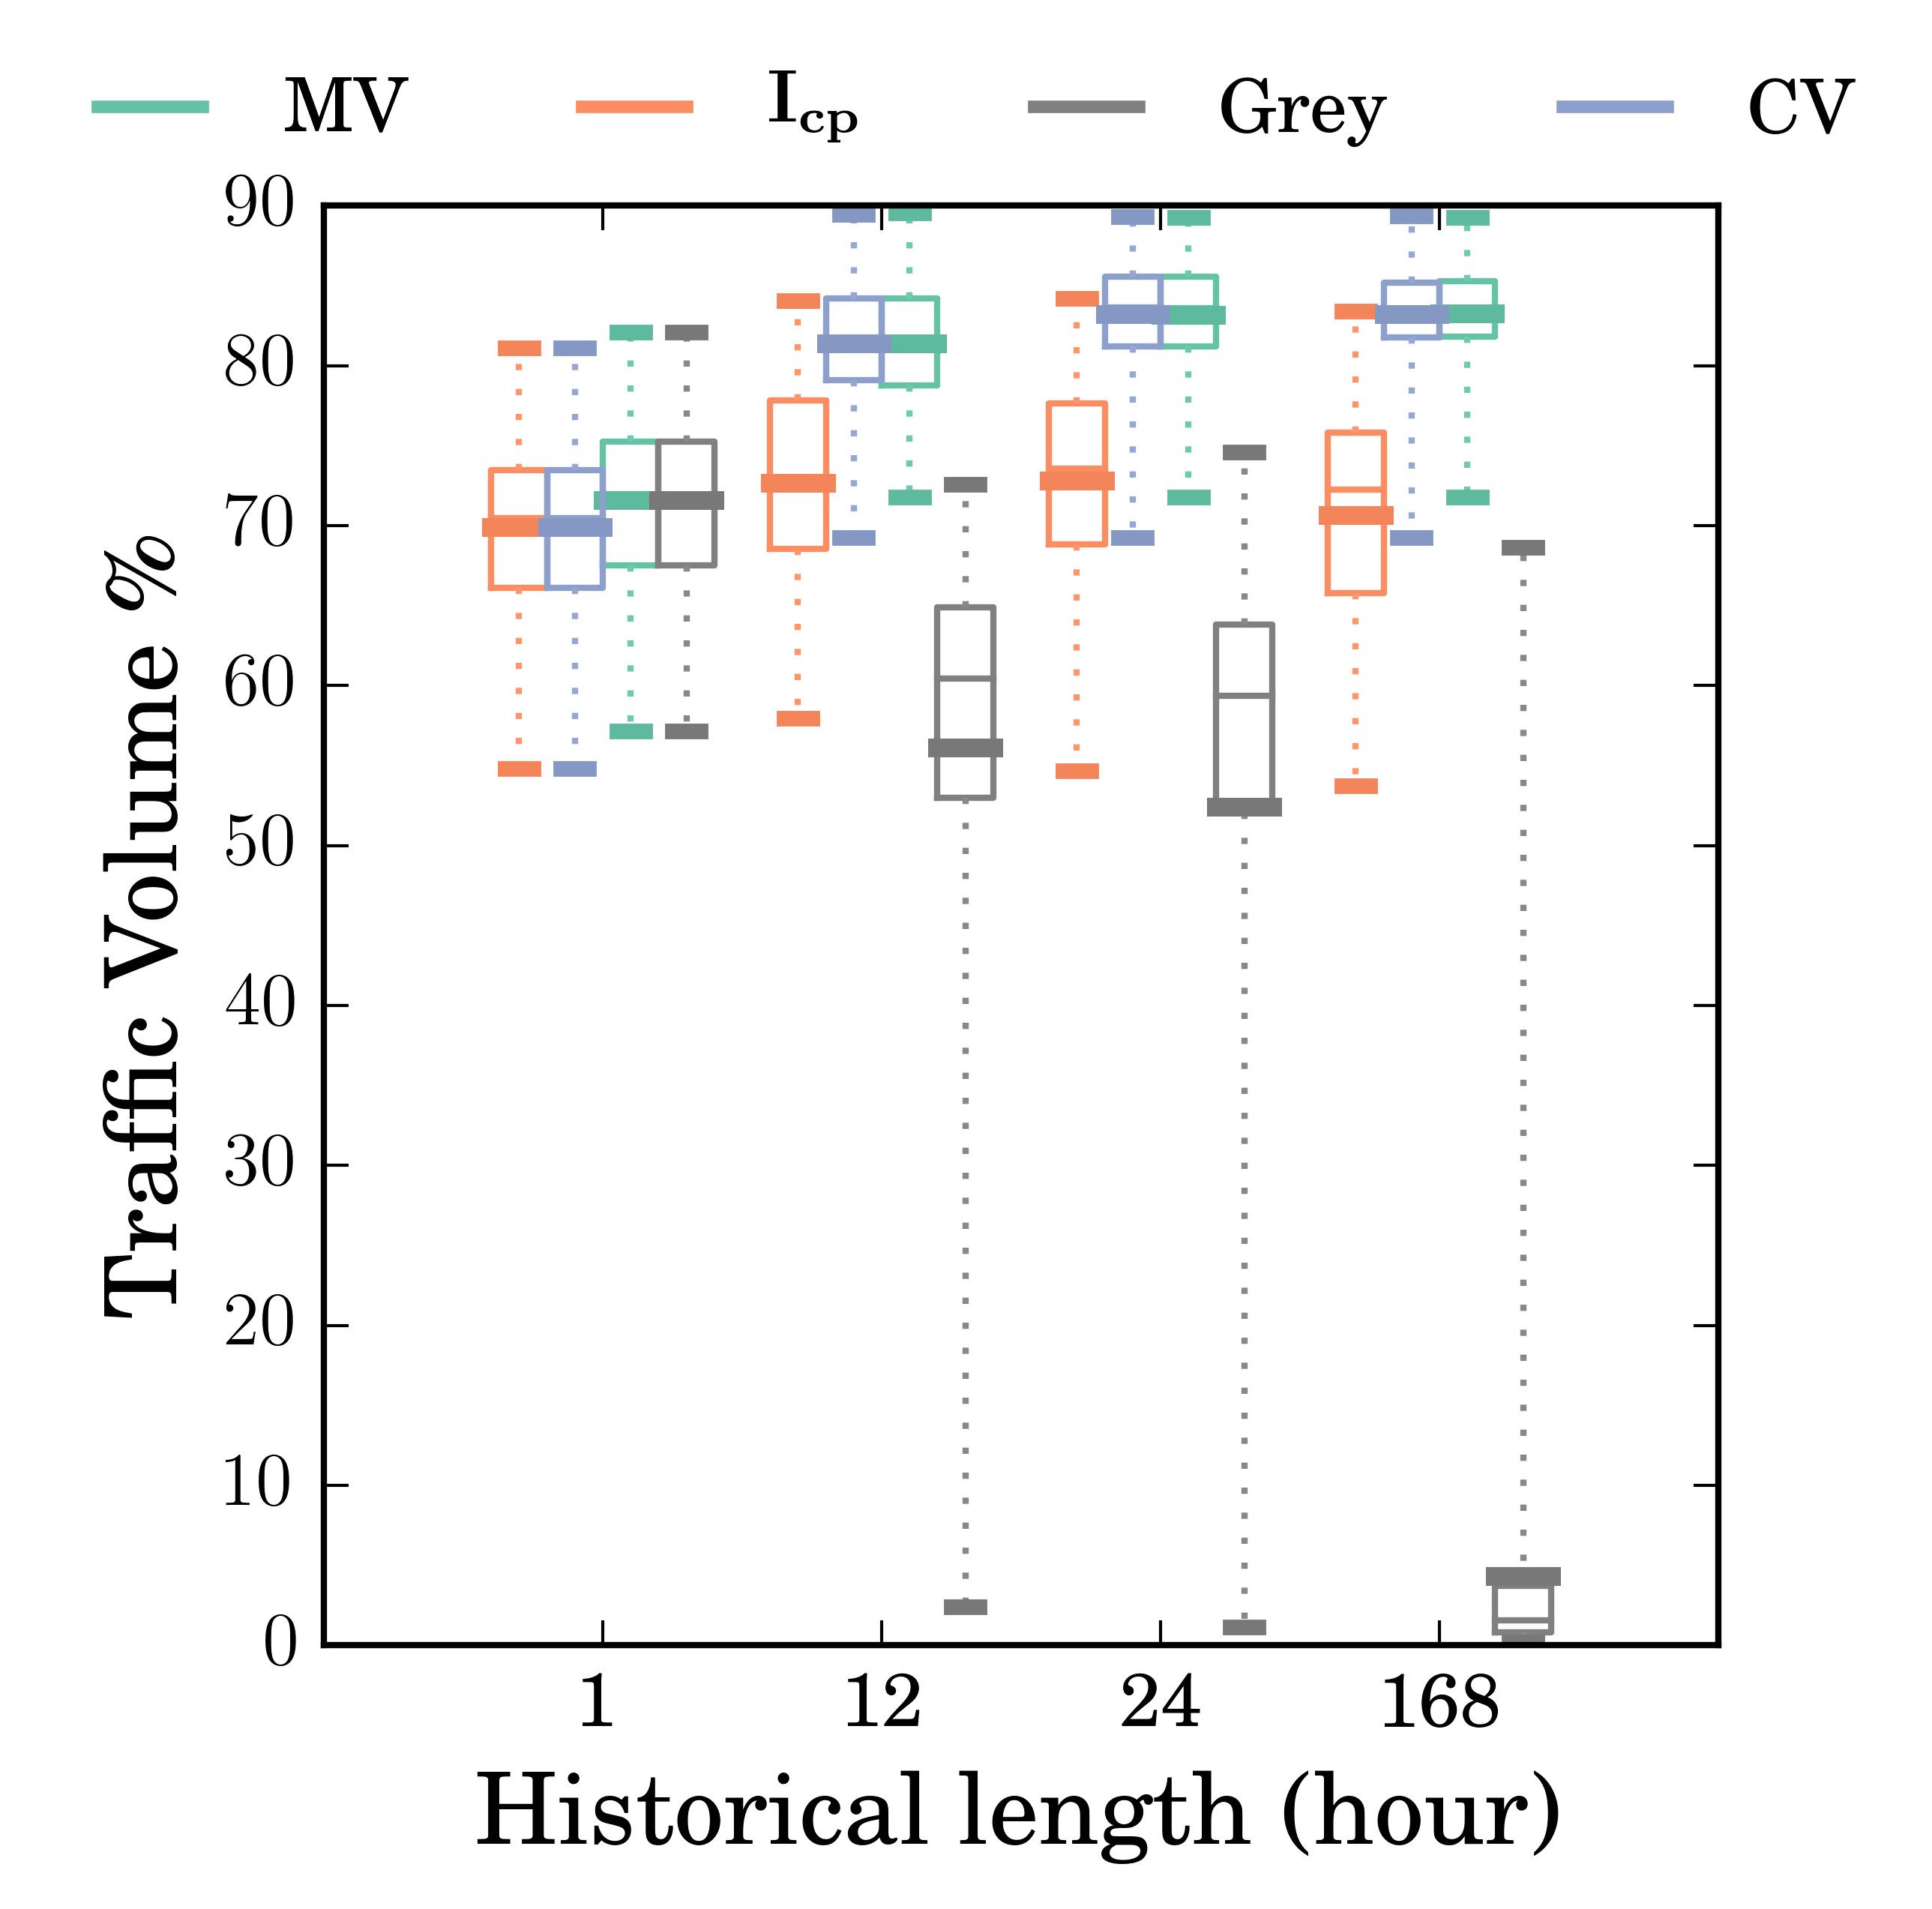
\includegraphics[width=\textwidth]{gfx/chap2/grey_cvg_box_method_compare_fs_sd.png}
                \caption{SD}
                \label{fig:cvg_sd}
        \end{subfigure}
        \begin{subfigure}[b]{0.48\textwidth}
                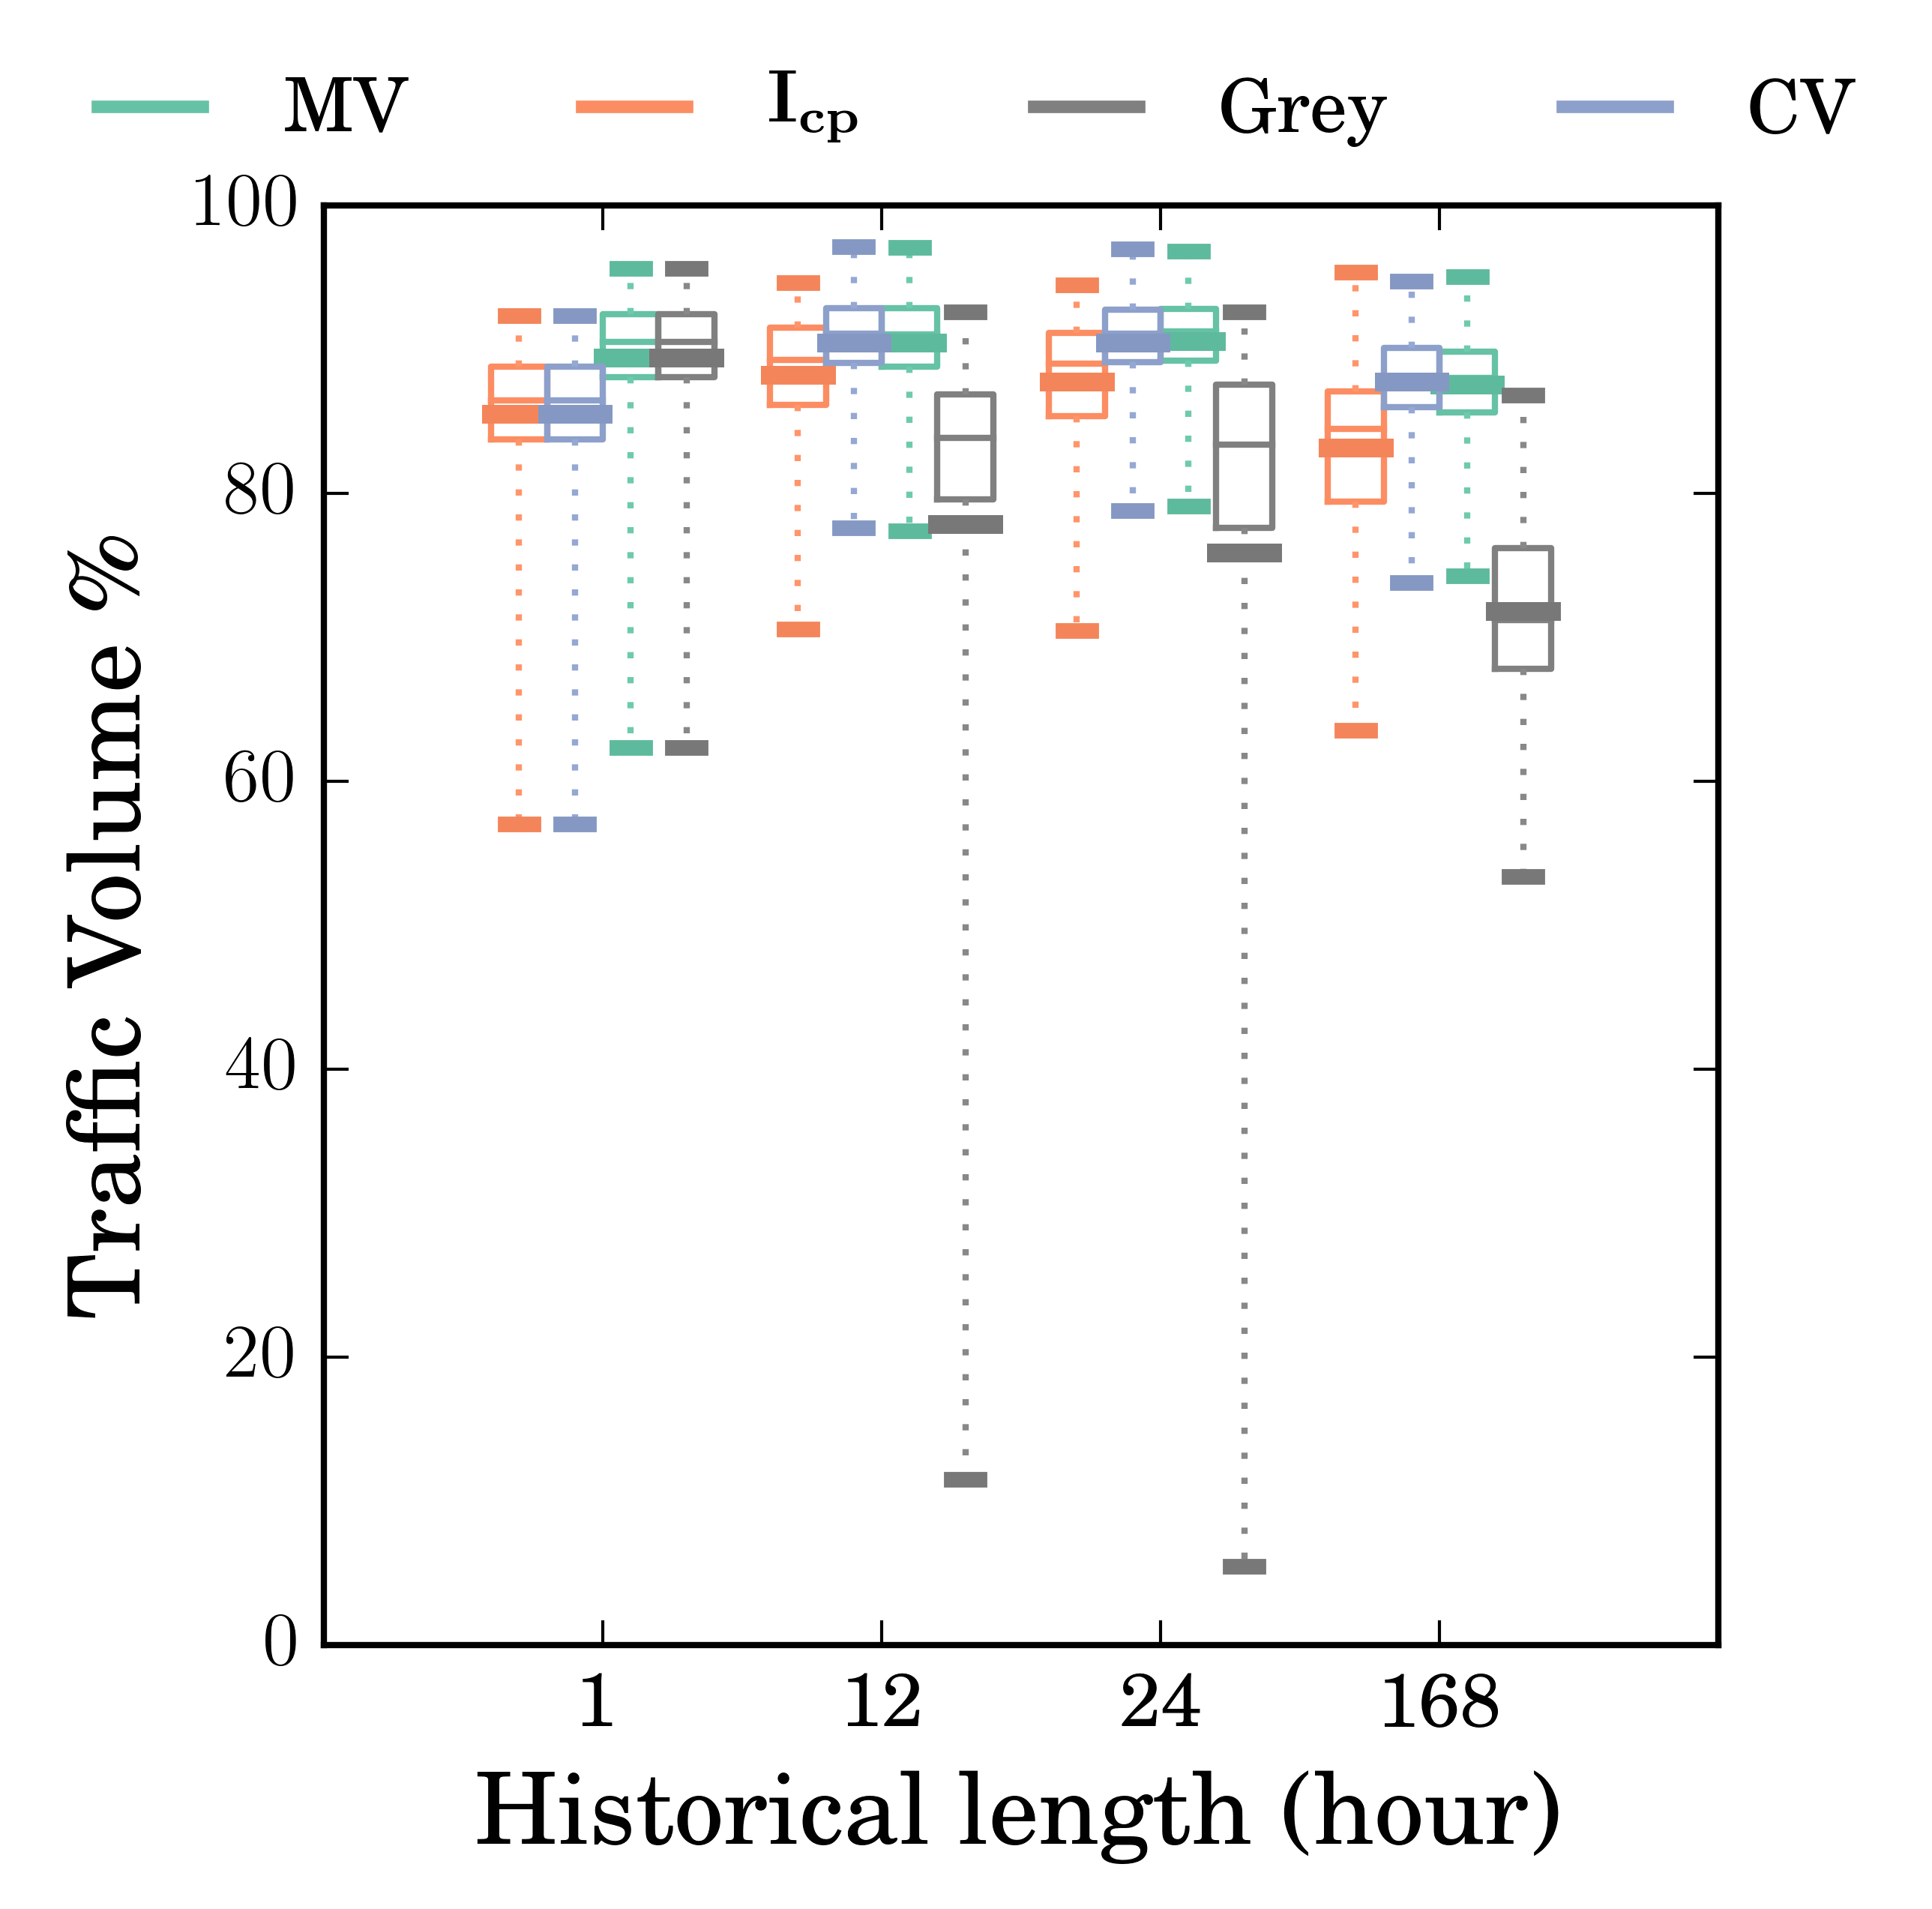
\includegraphics[width=\textwidth]{gfx/chap2/grey_cvg_box_method_compare_fs_se.png}
                \caption{SE}
                \label{fig:cvg_se}
        \end{subfigure}
        \begin{subfigure}[b]{0.48\textwidth}
                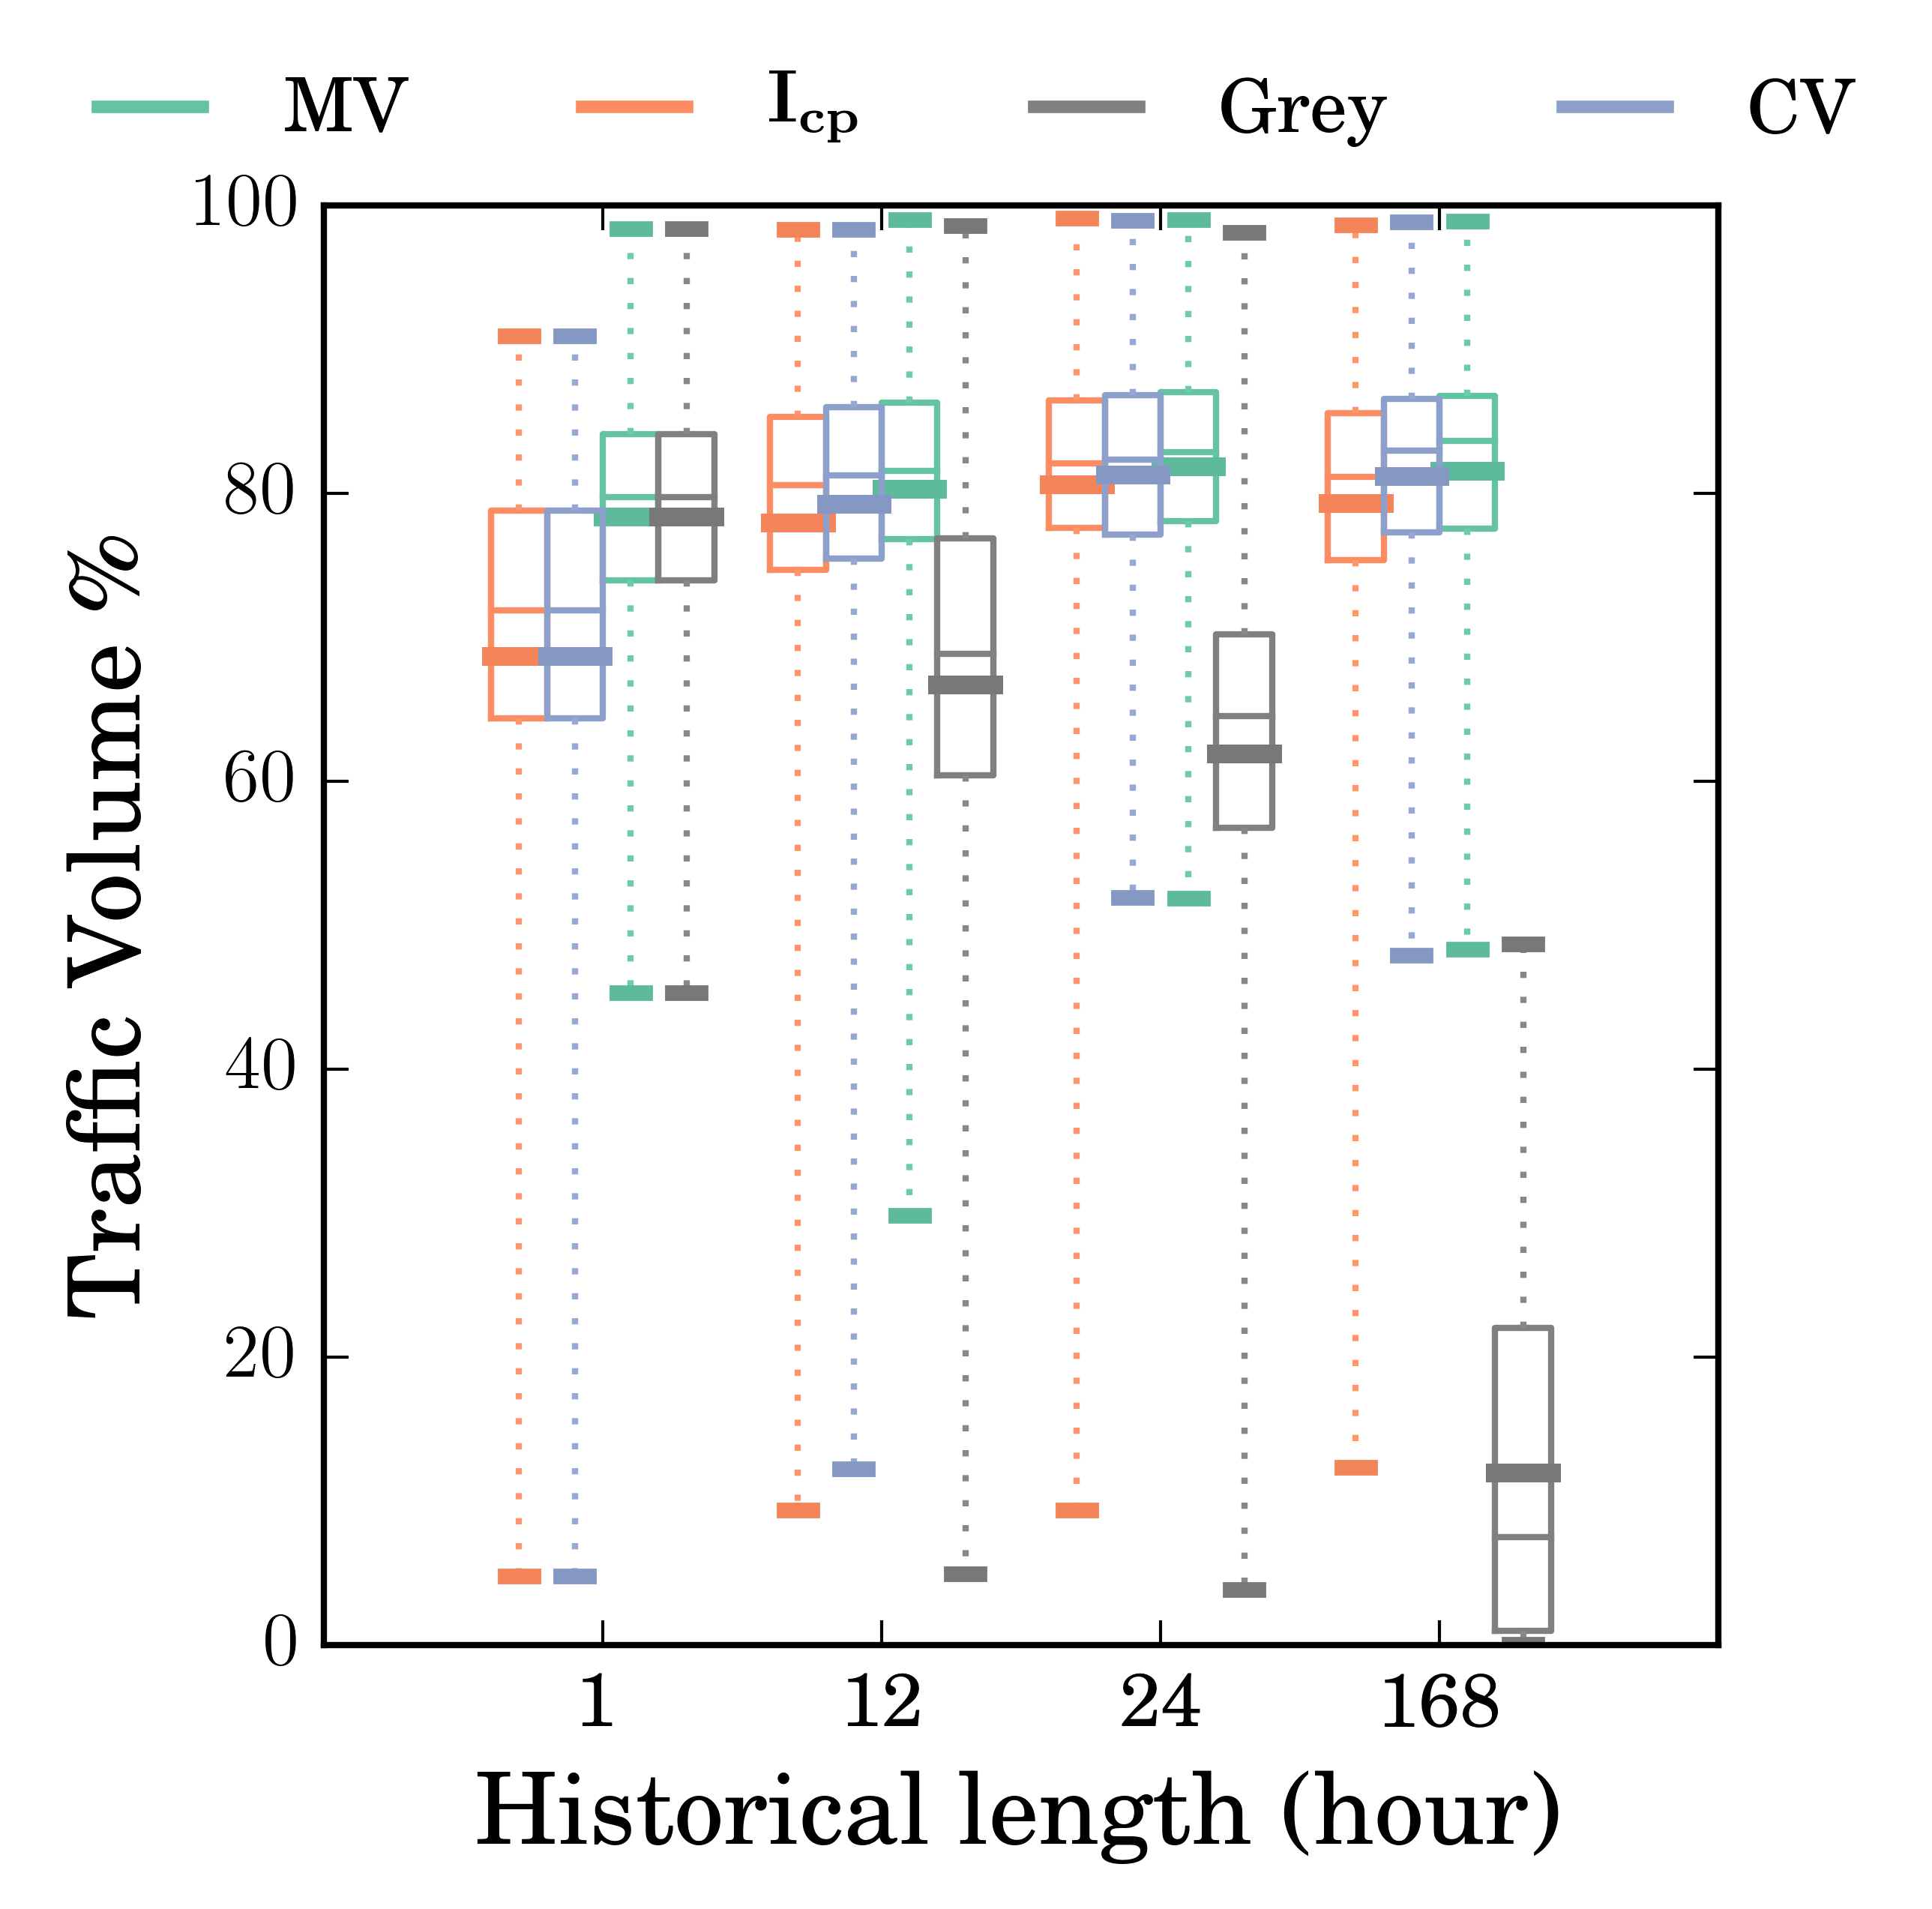
\includegraphics[width=\textwidth]{gfx/chap2/grey_cvg_box_method_compare_fs_sf.png}
                \caption{SF}
                \label{fig:cvg_sf}
        \end{subfigure}
\caption{Hour volume fraction covered by prefixes predictively selected using historical records of different lengths. The selection set size of each network is set to the maximum \textit{core} size over the week starting from June 1st, 2015, see in Table~\ref{tab:core_size}.}
\label{fig:cvg}
\end{figure}

\begin{figure}\ContinuedFloat
        \begin{subfigure}[b]{0.48\textwidth}
                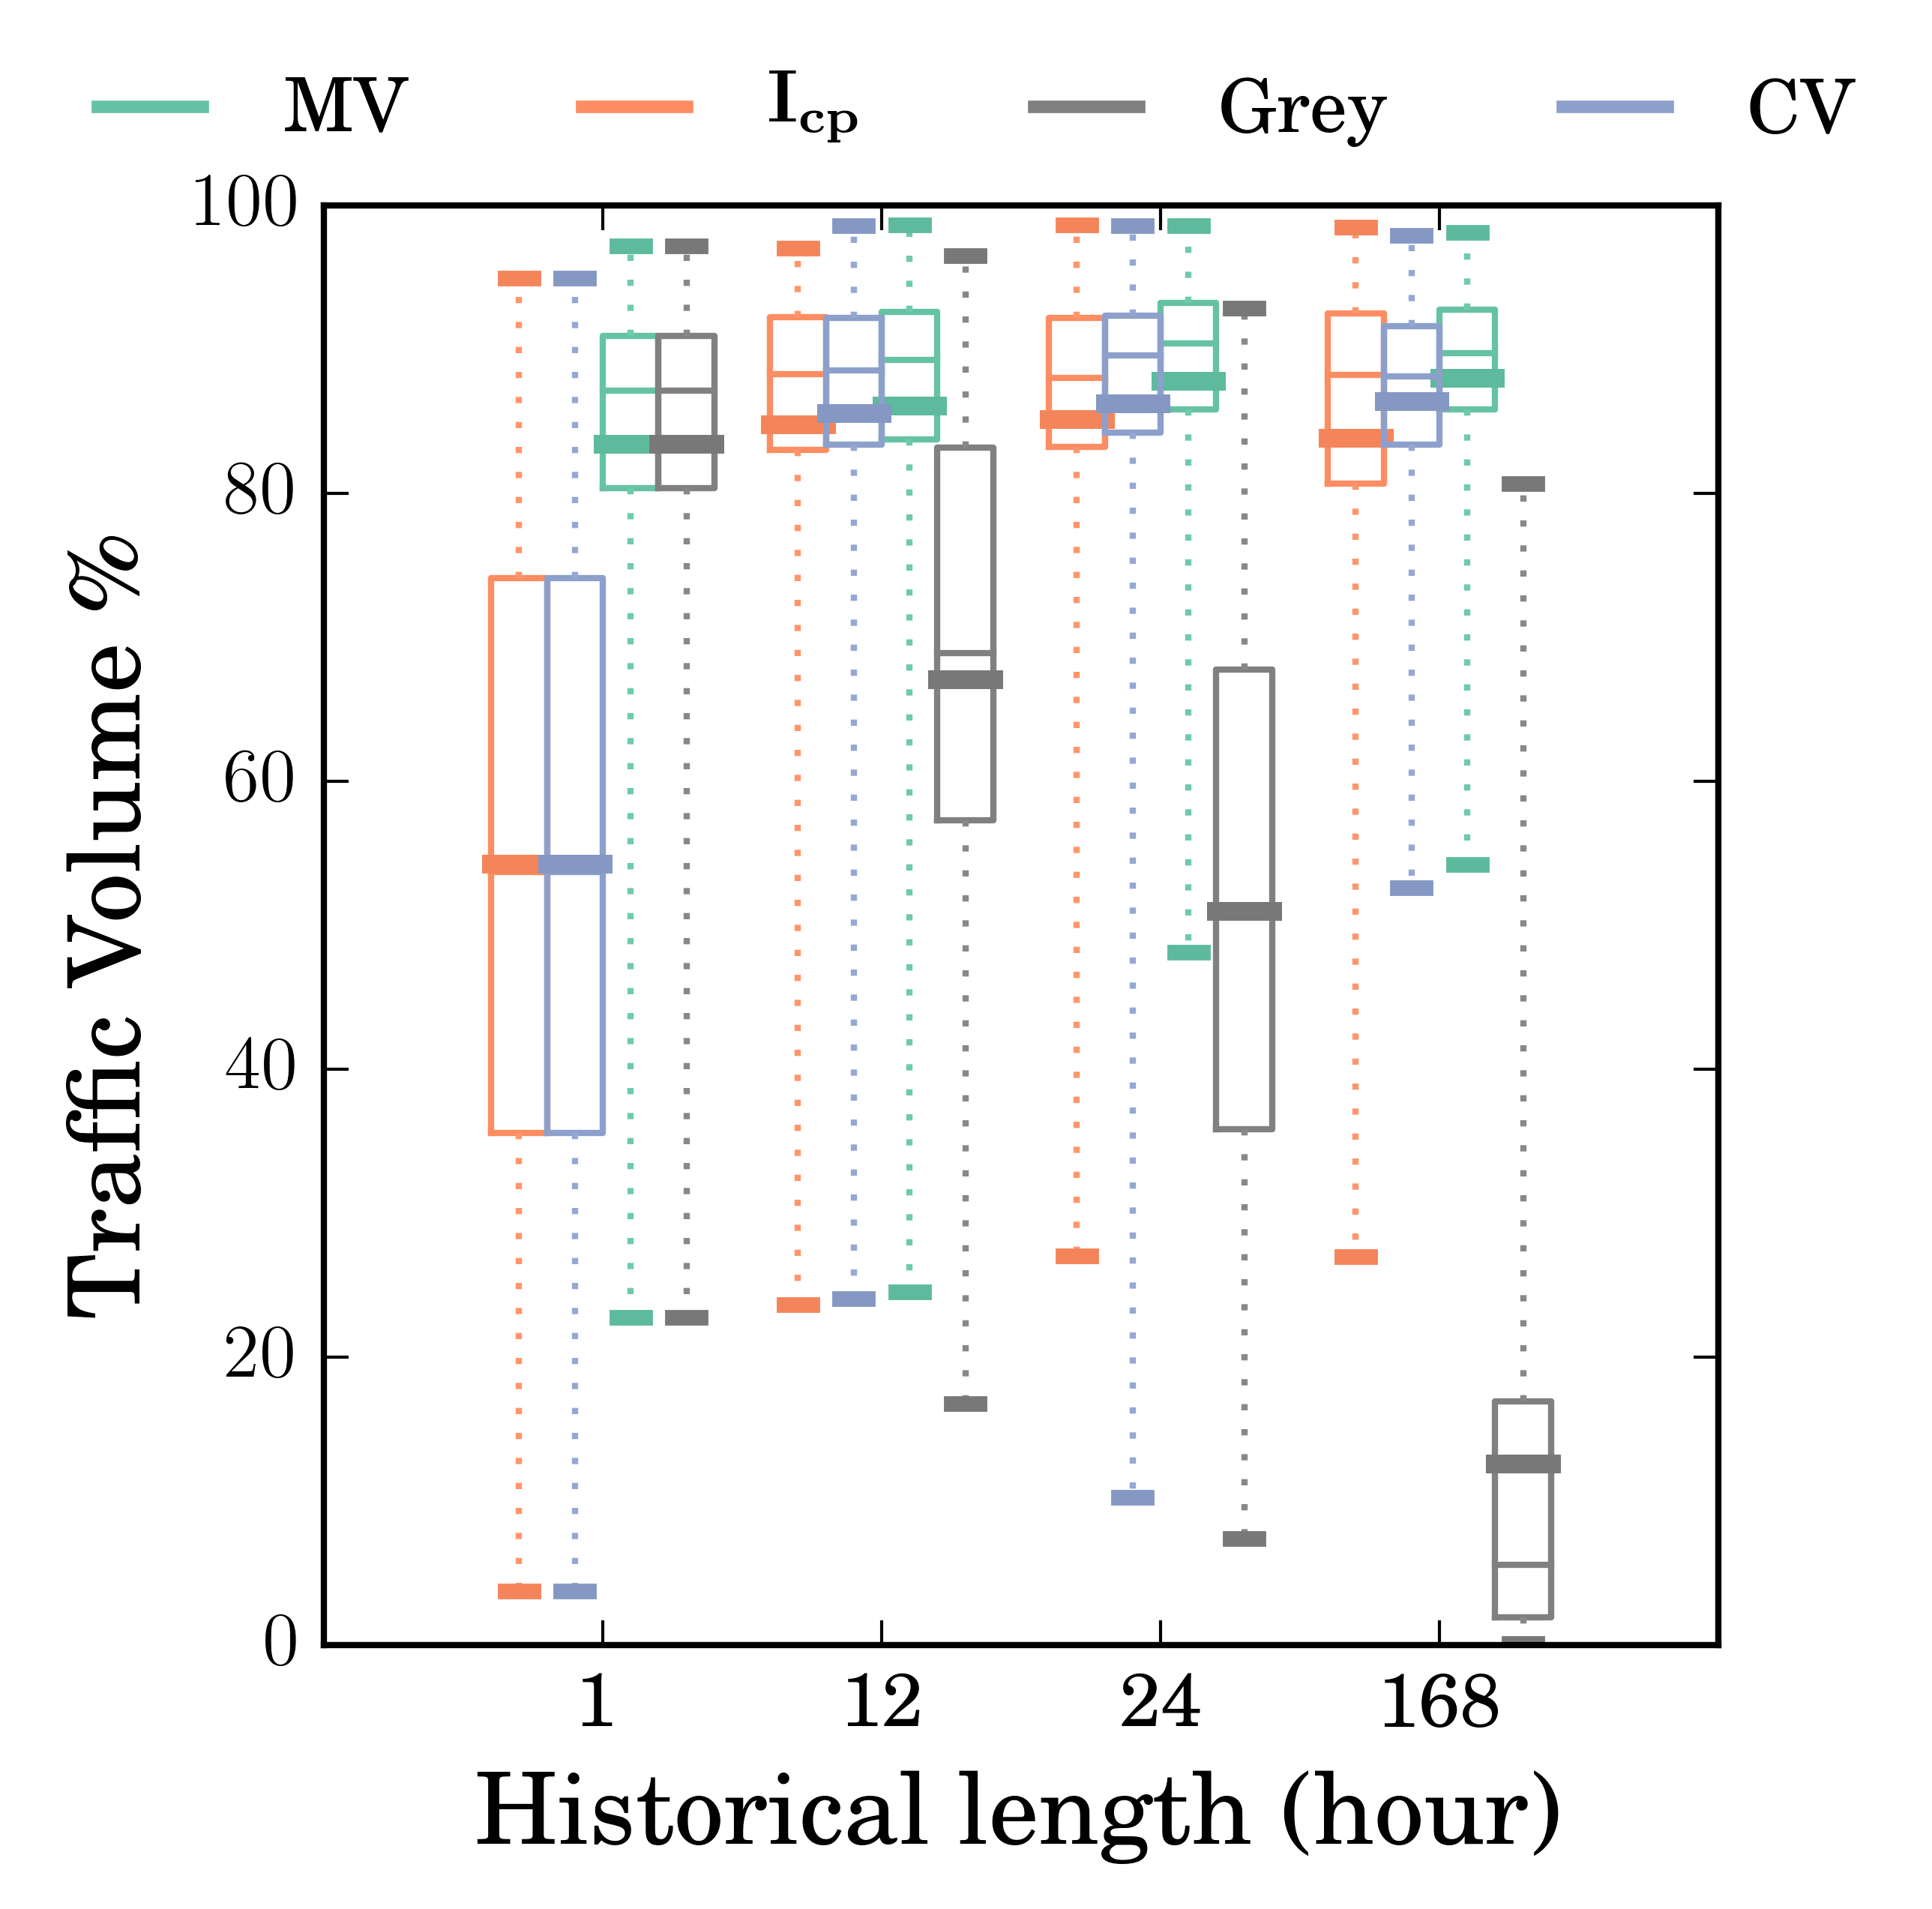
\includegraphics[width=\textwidth]{gfx/chap2/grey_cvg_box_method_compare_fs_sg.png}
                \caption{SG}
                \label{fig:cvg_sg}
        \end{subfigure}
        \begin{subfigure}[b]{0.48\textwidth}
                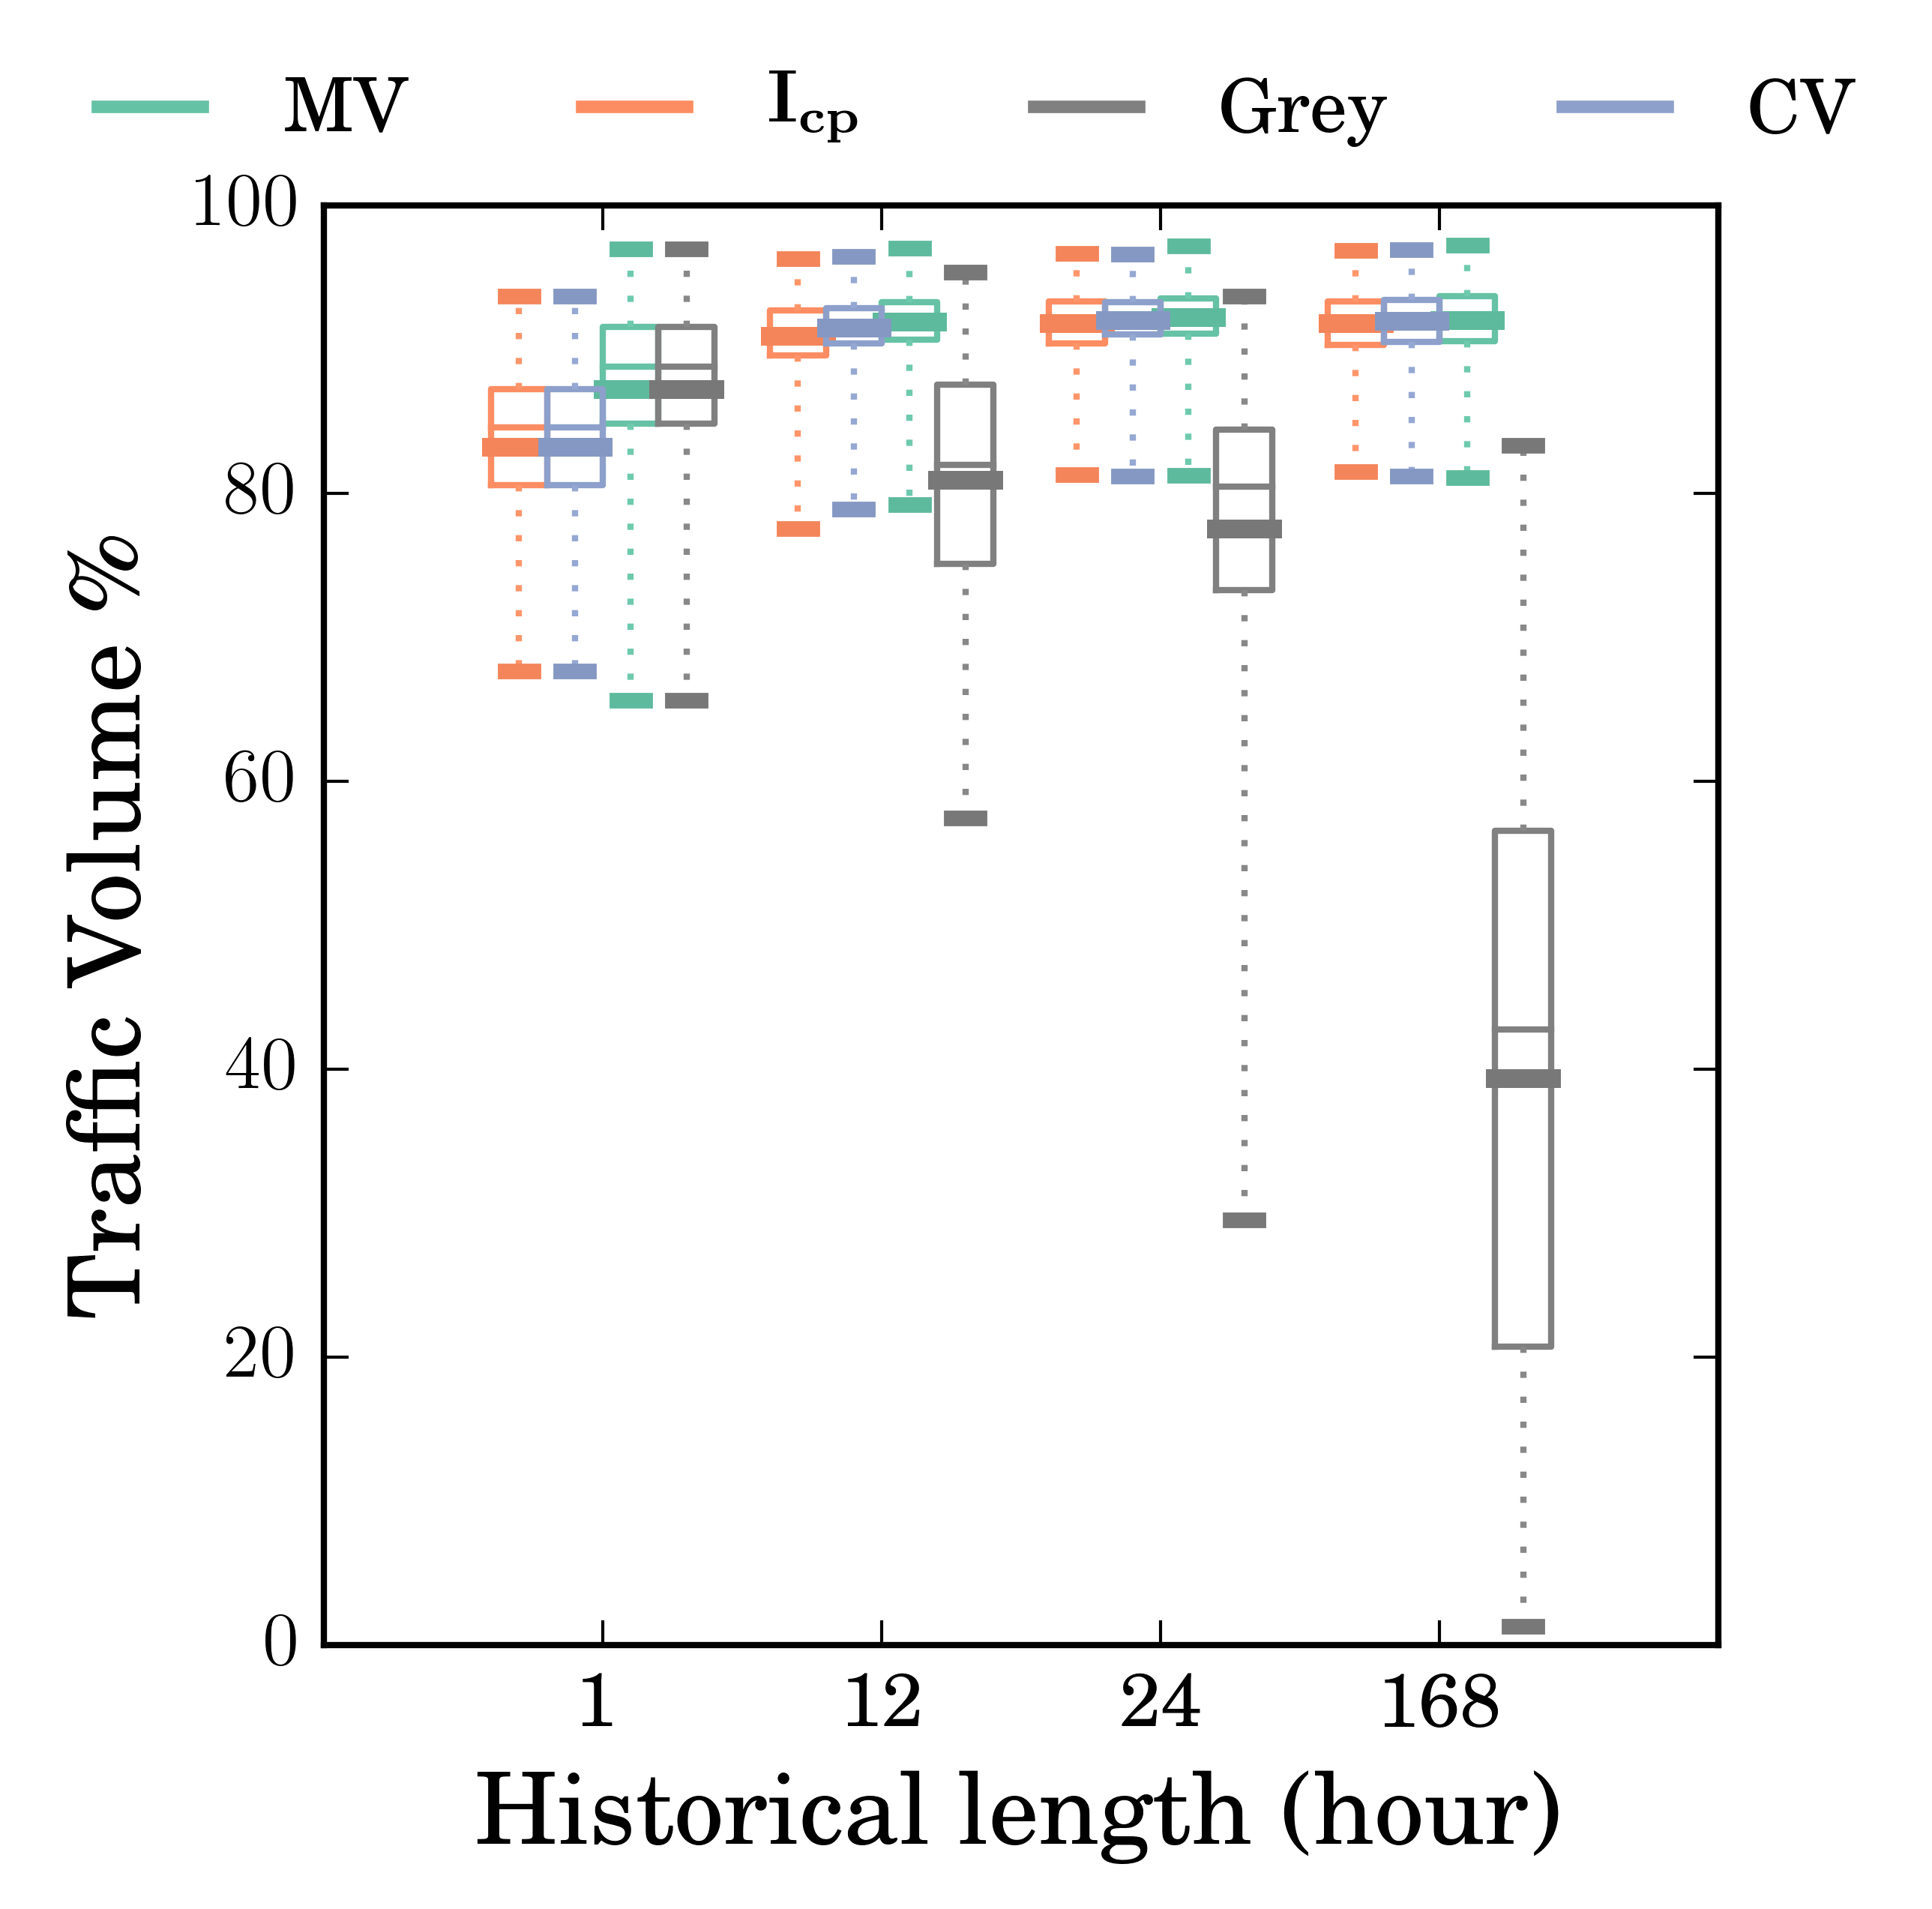
\includegraphics[width=\textwidth]{gfx/chap2/grey_cvg_box_method_compare_fs_sh.png}
                \caption{SH}
                \label{fig:cvg_sh}
        \end{subfigure}
        \begin{subfigure}[b]{0.48\textwidth}
                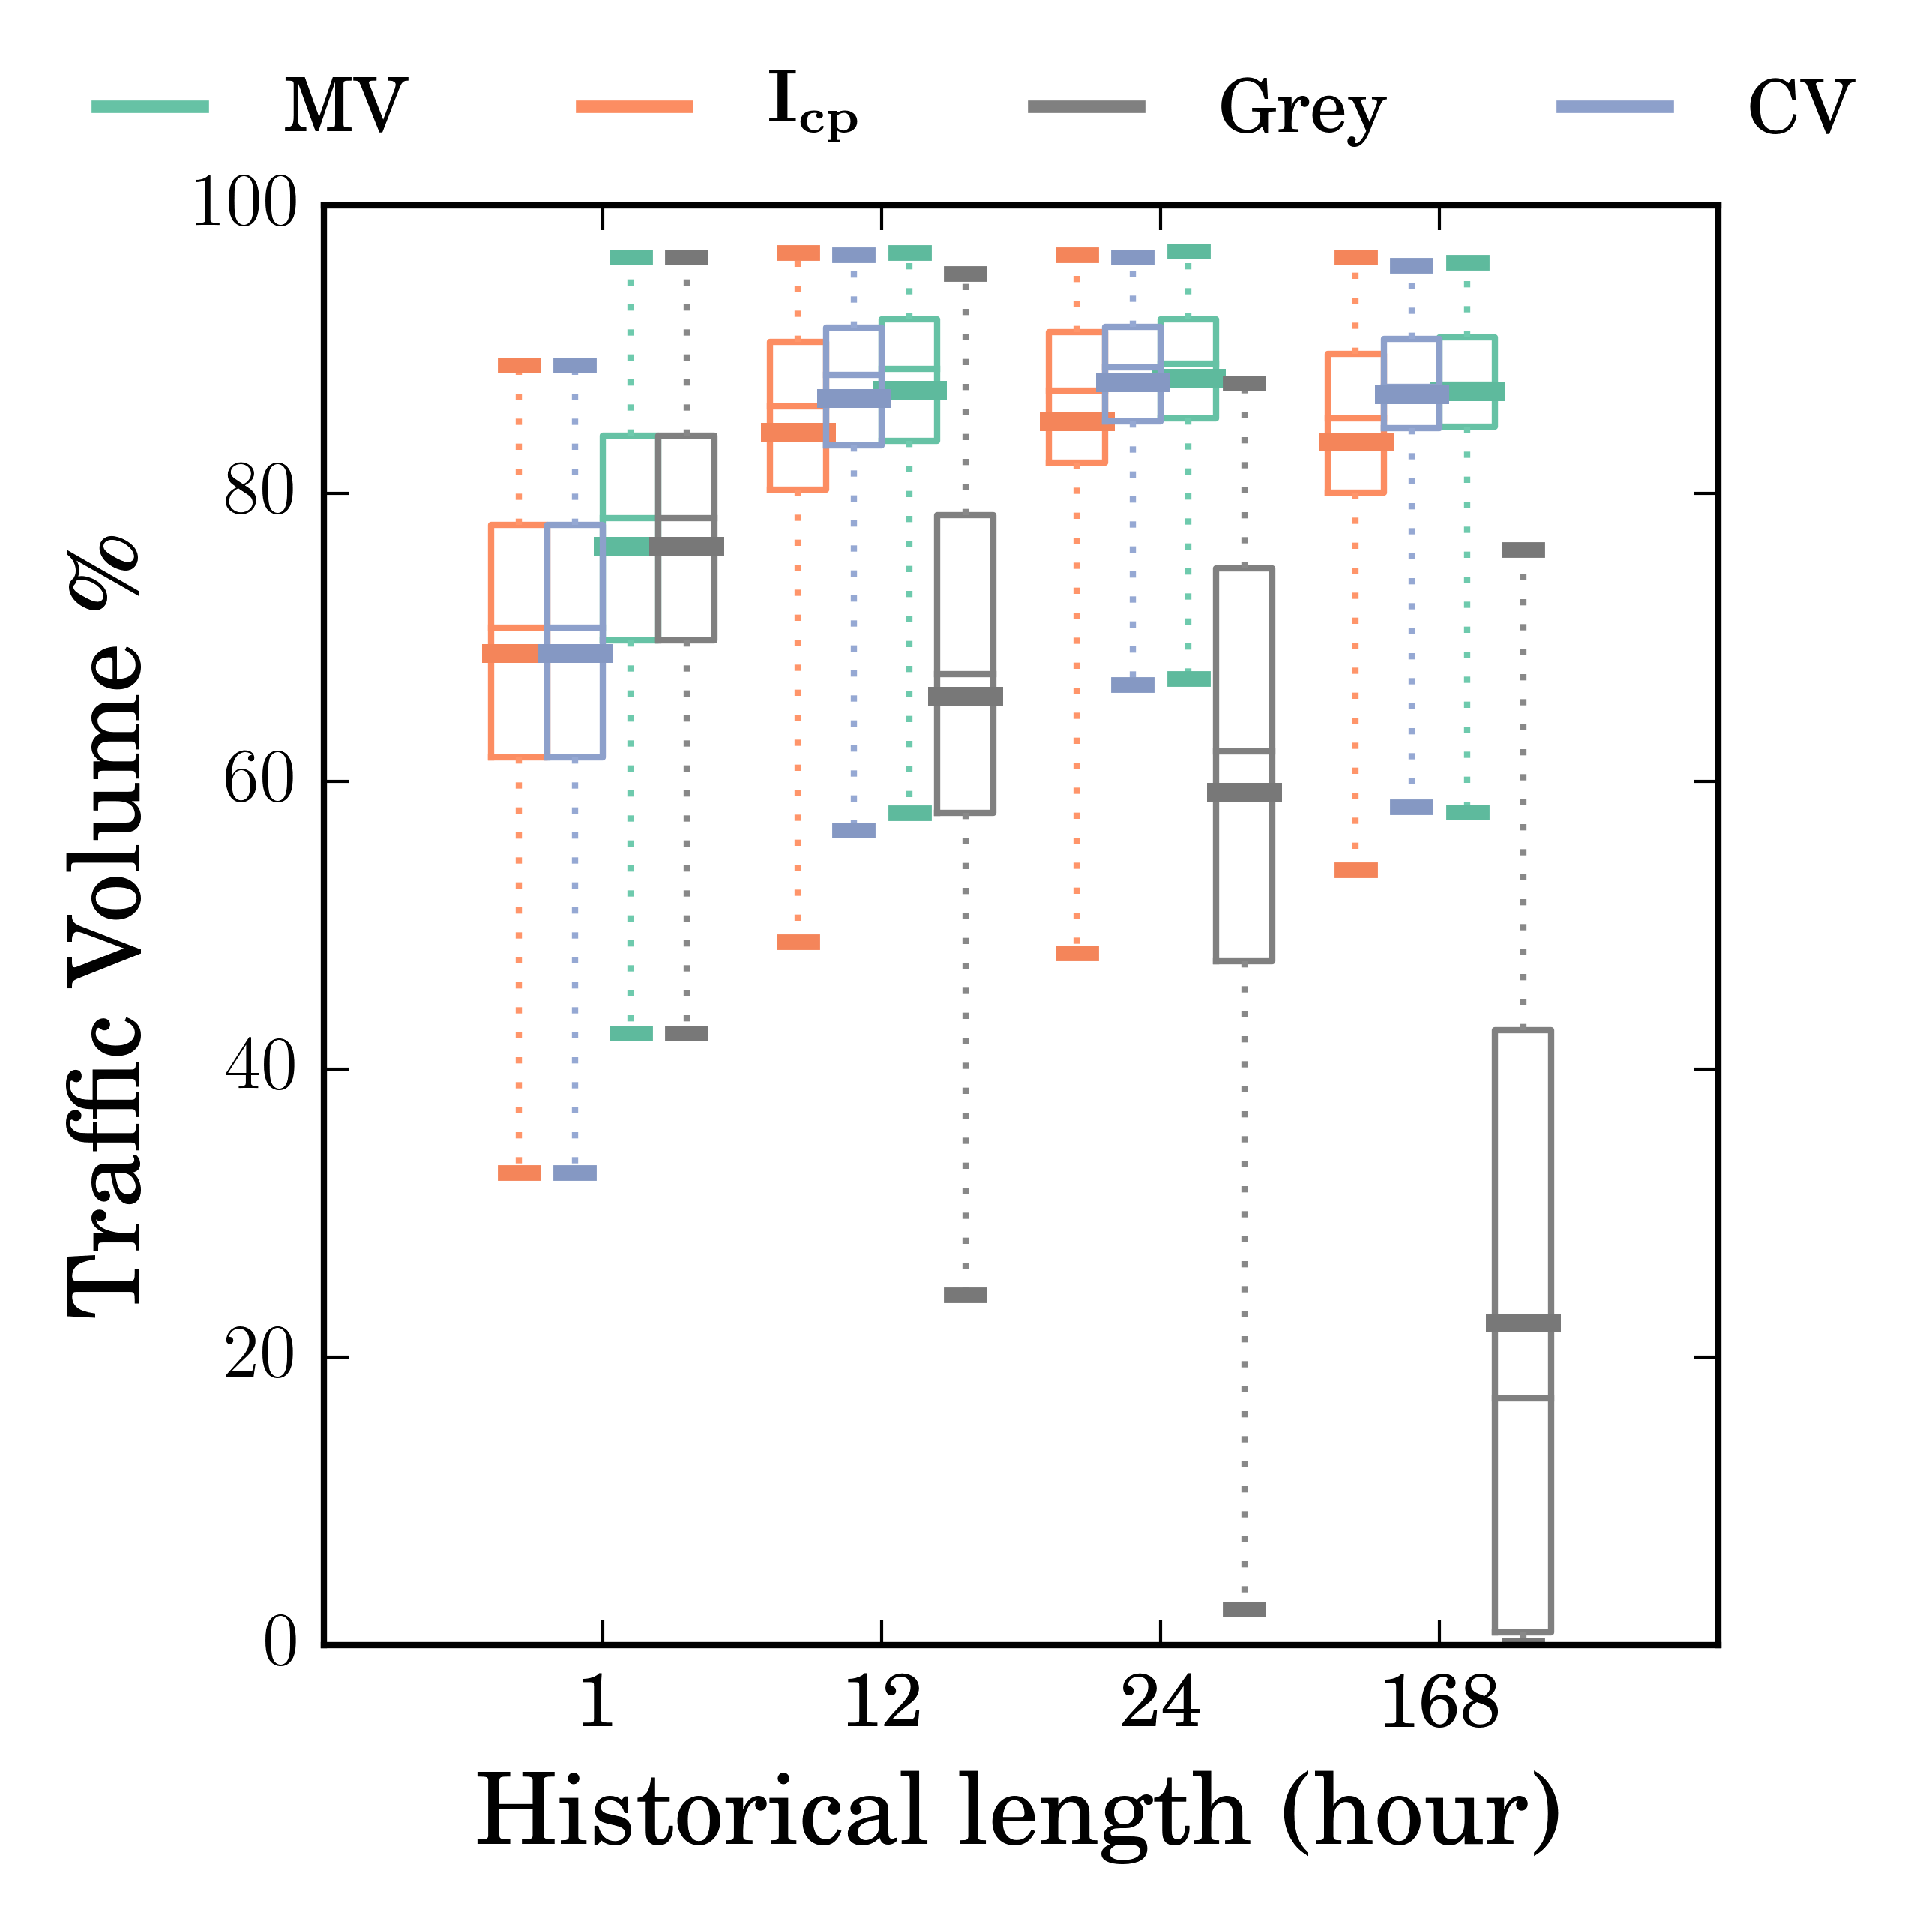
\includegraphics[width=\textwidth]{gfx/chap2/grey_cvg_box_method_compare_fs_si.png}
                \caption{SI}
                \label{fig:cvg_si}
        \end{subfigure}
\caption{(cont.) Hour volume fraction covered by prefixes predictively selected using historical records of different lengths.}
\label{fig:cvg_cont}
\end{figure}

\marginpar{volume coverage}
In evaluating and comparing the performance of these methods, we fixed the selection set size to the maximum \textit{core} size over the week. 
Fig.~\ref{fig:cvg} illustrates the hour volume coverage by the four methods in the form of box-plot, representing the minimum, maximum, 25th and 75th percentile, medium and mean values. 
Among proposed metrics, we find that the $CV$ is very close to $MV$ in terms of volume coverage, proving that it is a good approximation of the later, while being more resource economical.

Basing solely on the last 1 hour records, all methods yield already a mean volume coverage $>80\%$ on SA, SB, SE and SH, which implies a strong continuity on prefix volumes between two consecutive hours. 
On SC and SG, however, using records of last 168 hours, i.e. a week, offers much better minimum volume coverage than shorter records. This is due to the fact that at certain hour, SC and SG undergo a great amount of bursty traffic (as observed previously, e.g. in Table~\ref{tab:bi} and Fig.~\ref{fig:cv_cp}). By increasing the historical length, the selection metrics are able to have better visibility into the past and capture some of these bursty prefixes ---  finally improving the minimum coverage.
This gain in minimum volume coverage by using long historical records can actually be observed on all networks, between 1 hour and 12 hours, also between 12 hour and 24 hour. 
However from 24 hour to 168, this gain doesn't necessary happen on all sites, which is due to the fact that the total volume brought by some highly bursty prefix is diluted by the long time span using $MV$ and $CV$ metrics. In order to capture them, a larger selection set size is need, which inevitably includes more prefixes of few significance.


\begin{figure}
\centering
		\centering
		\begin{subfigure}[b]{0.9\textwidth}
                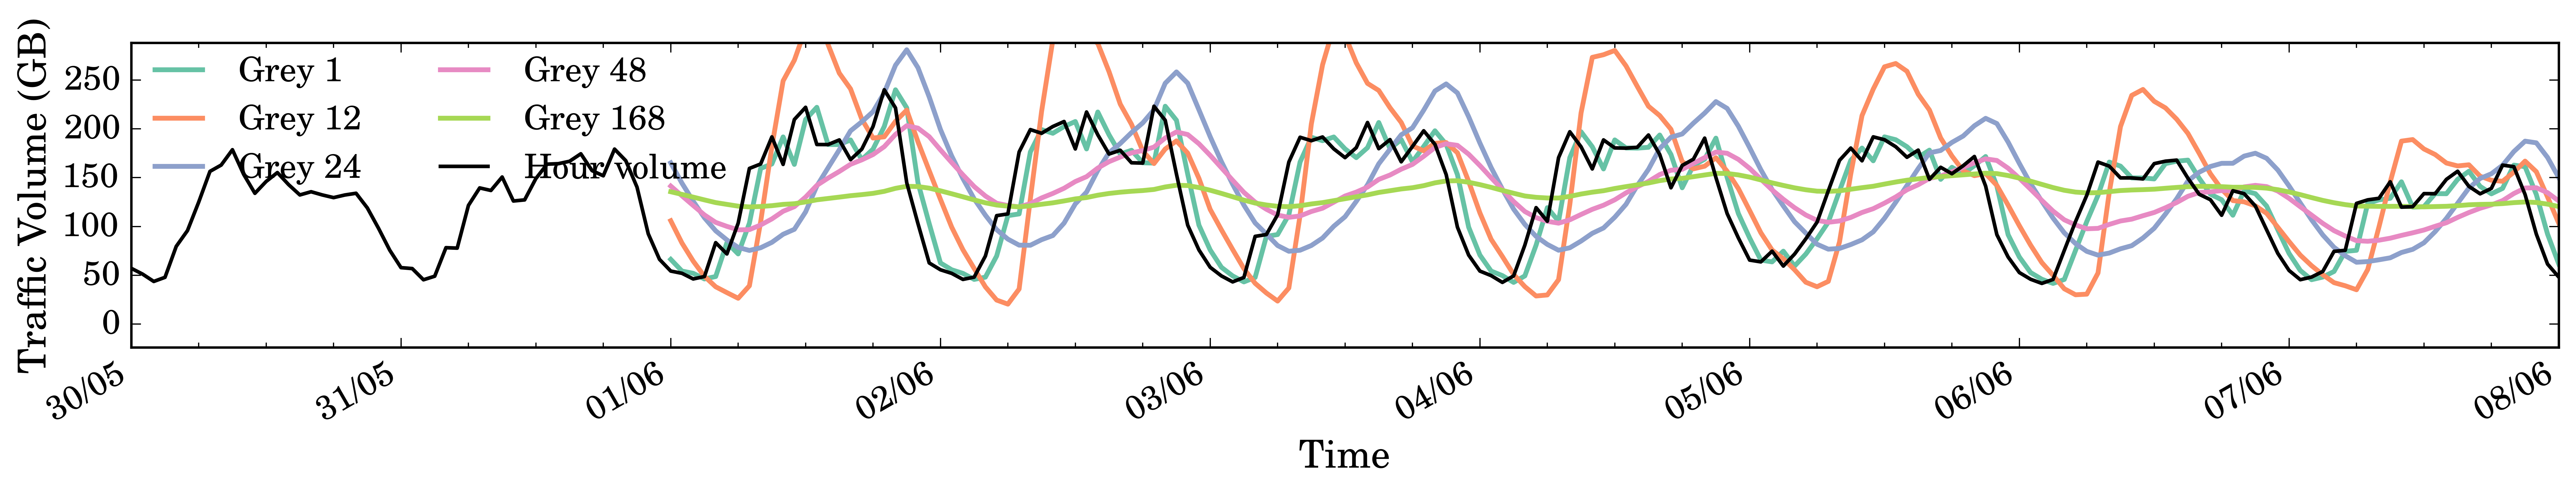
\includegraphics[width=\textwidth]{gfx/chap2/grey_sa.png}
                \caption{SA}
                \label{fig:grey_sa}
        \end{subfigure}
        \begin{subfigure}[b]{0.9\textwidth}
                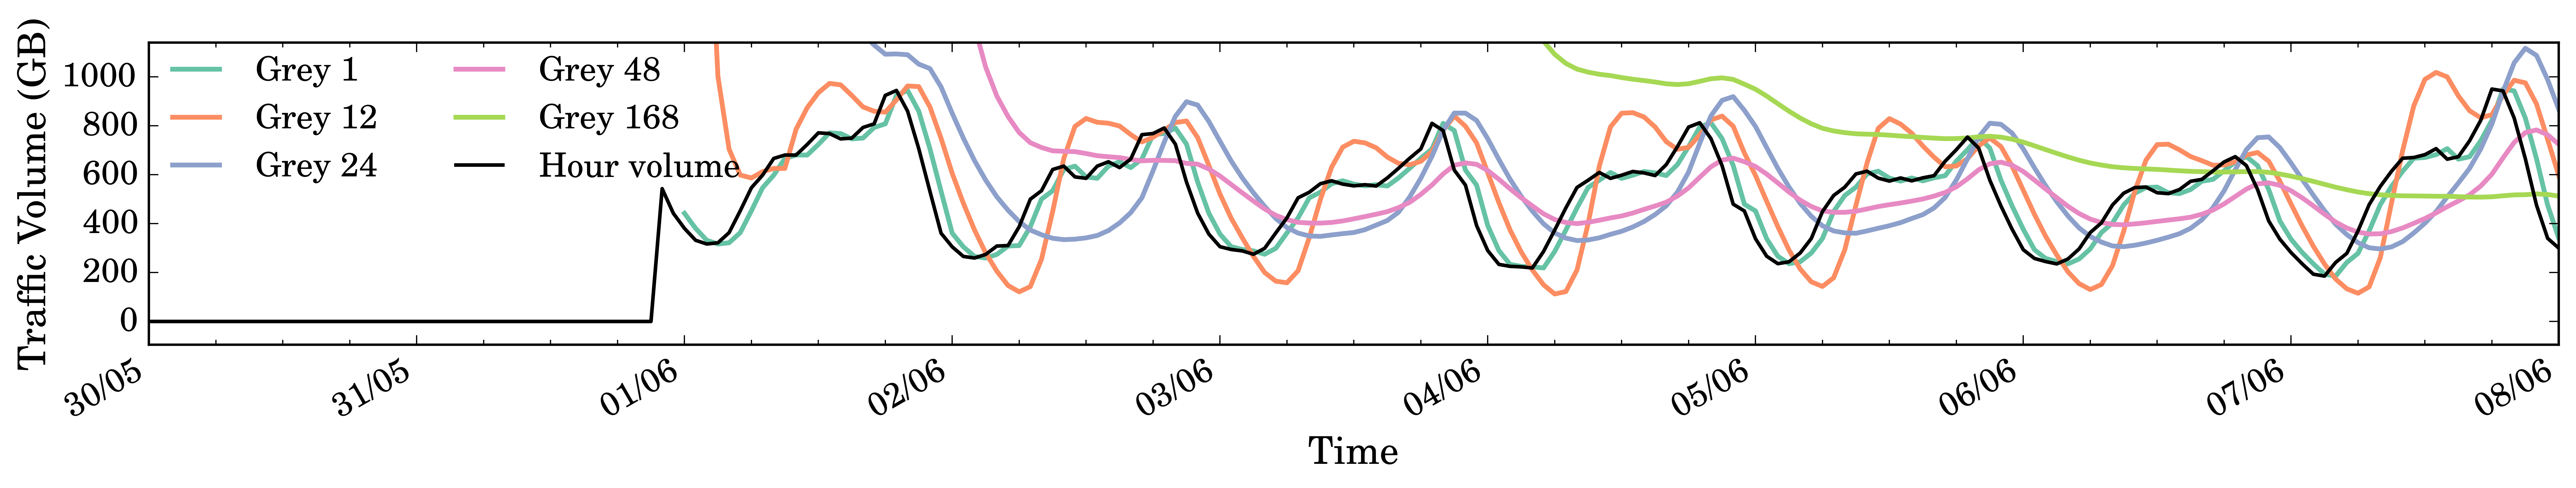
\includegraphics[width=\textwidth]{gfx/chap2/grey_sb.png}
                \caption{SB}
                \label{fig:grey_sb}
        \end{subfigure}
        \begin{subfigure}[b]{0.9\textwidth}
                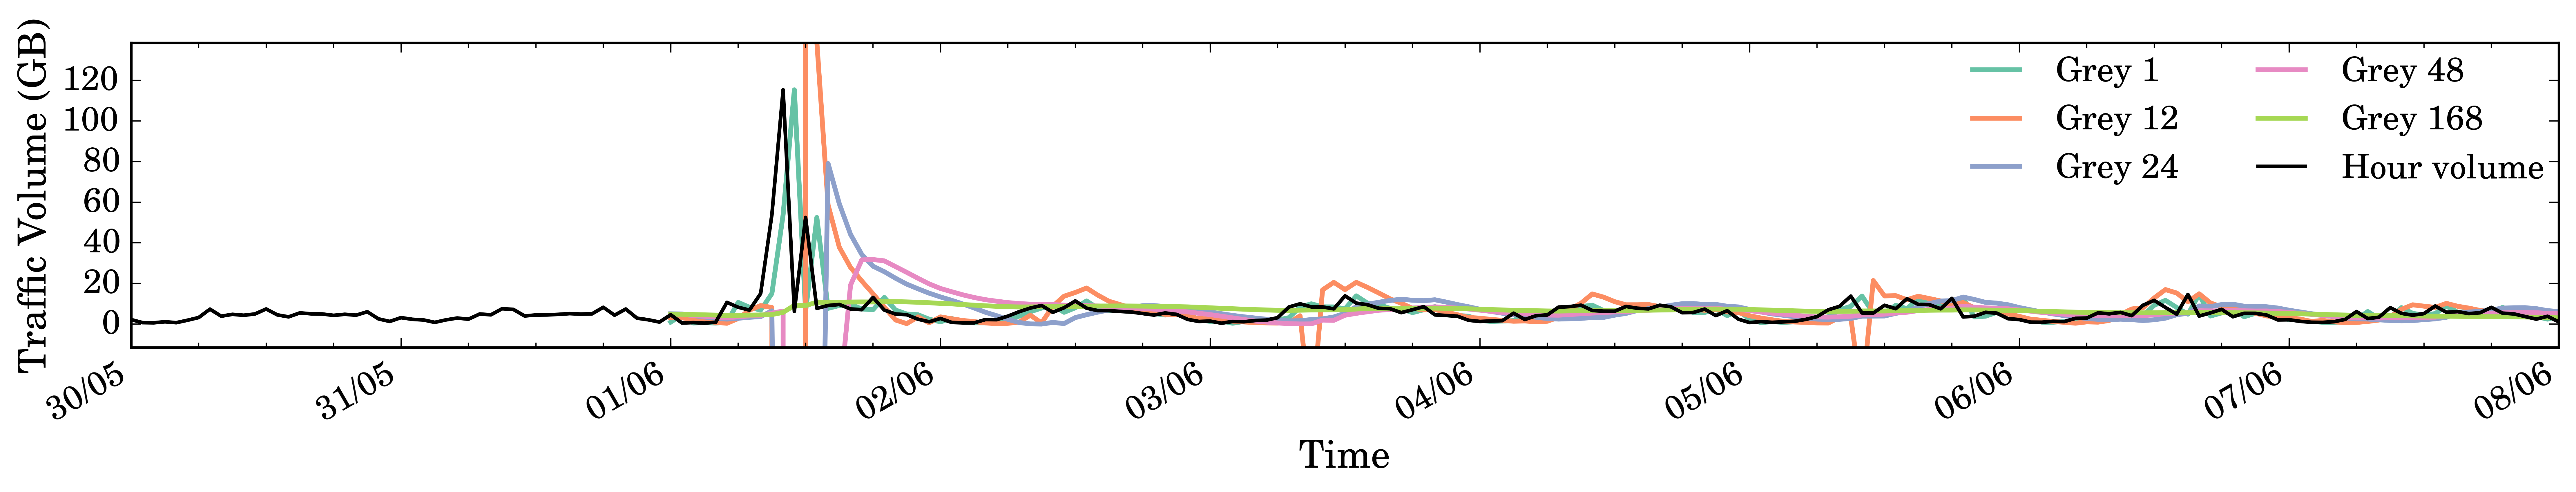
\includegraphics[width=\textwidth]{gfx/chap2/grey_sc.png}
                \caption{SC}
                \label{fig:grey_sc}
        \end{subfigure}
		\centering
        \begin{subfigure}[b]{0.9\textwidth}
                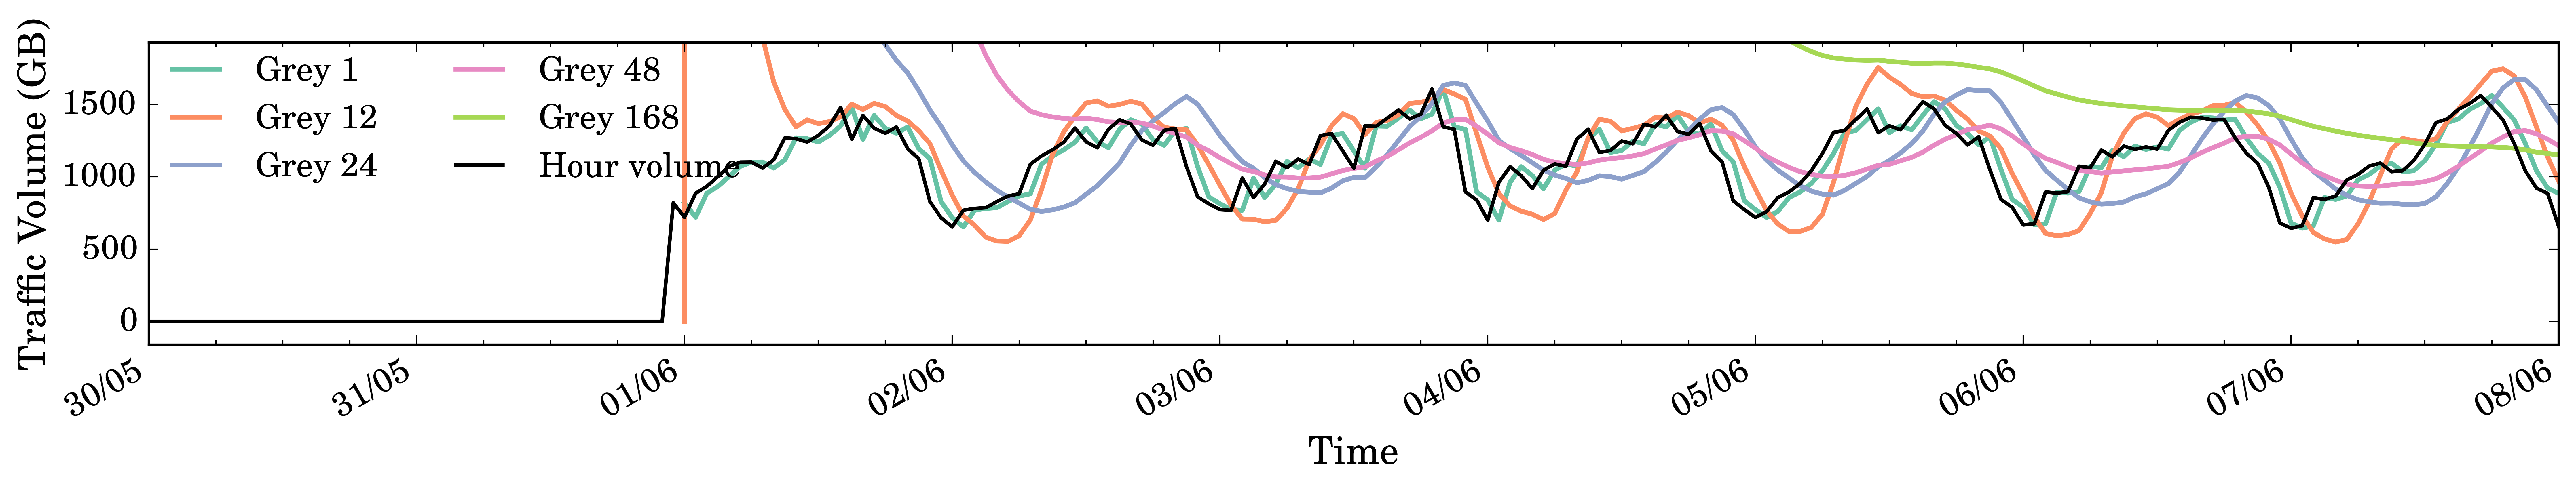
\includegraphics[width=\textwidth]{gfx/chap2/grey_sd.png}
                \caption{SD}
                \label{fig:grey_sd}
        \end{subfigure}
        \begin{subfigure}[b]{0.9\textwidth}
                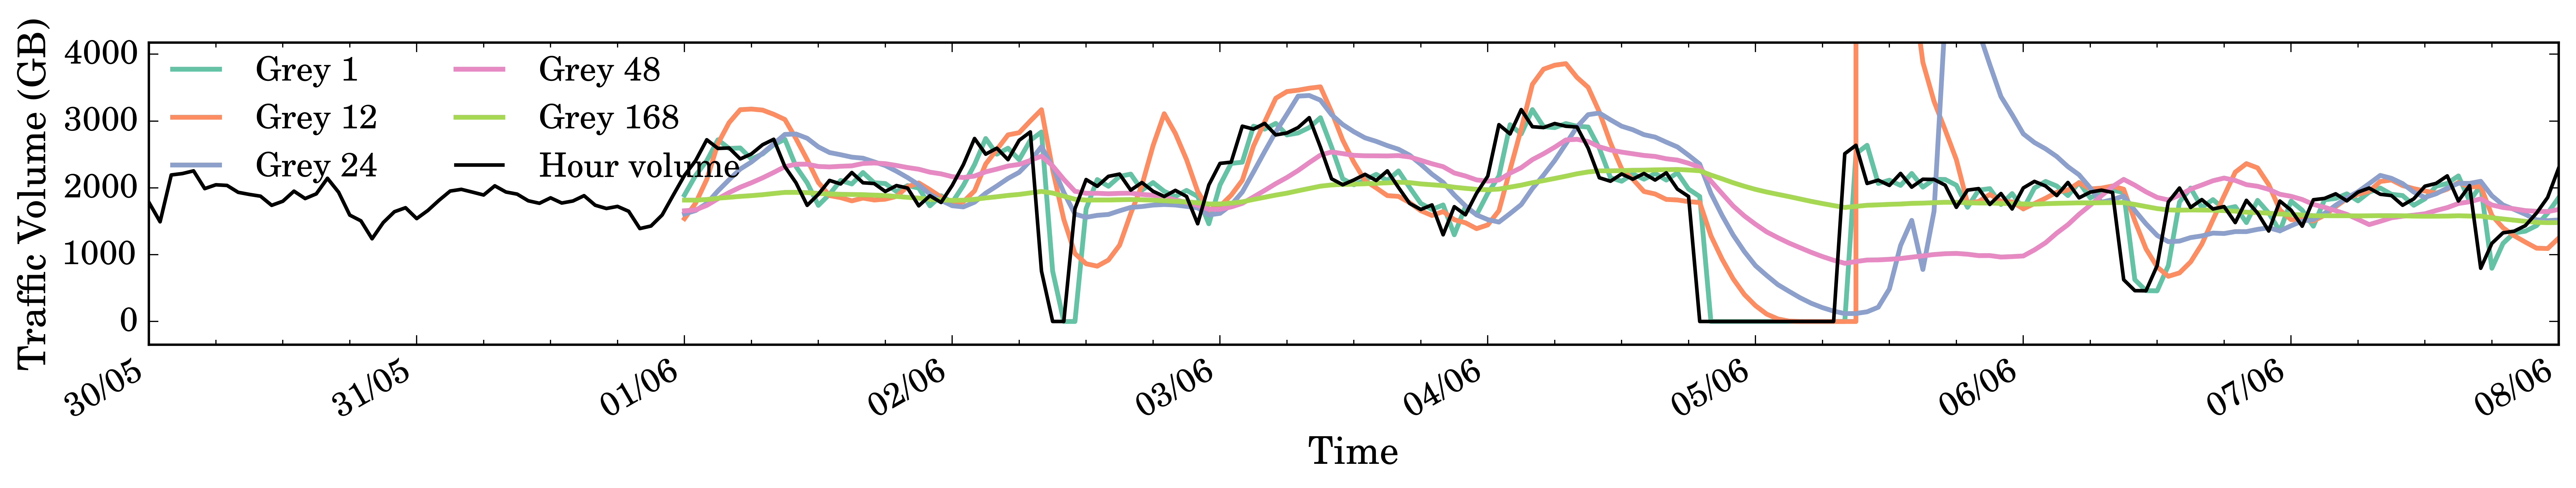
\includegraphics[width=\textwidth]{gfx/chap2/grey_se.png}
                \caption{SE}
                \label{fig:grey_se}
        \end{subfigure}
        \begin{subfigure}[b]{0.9\textwidth}
                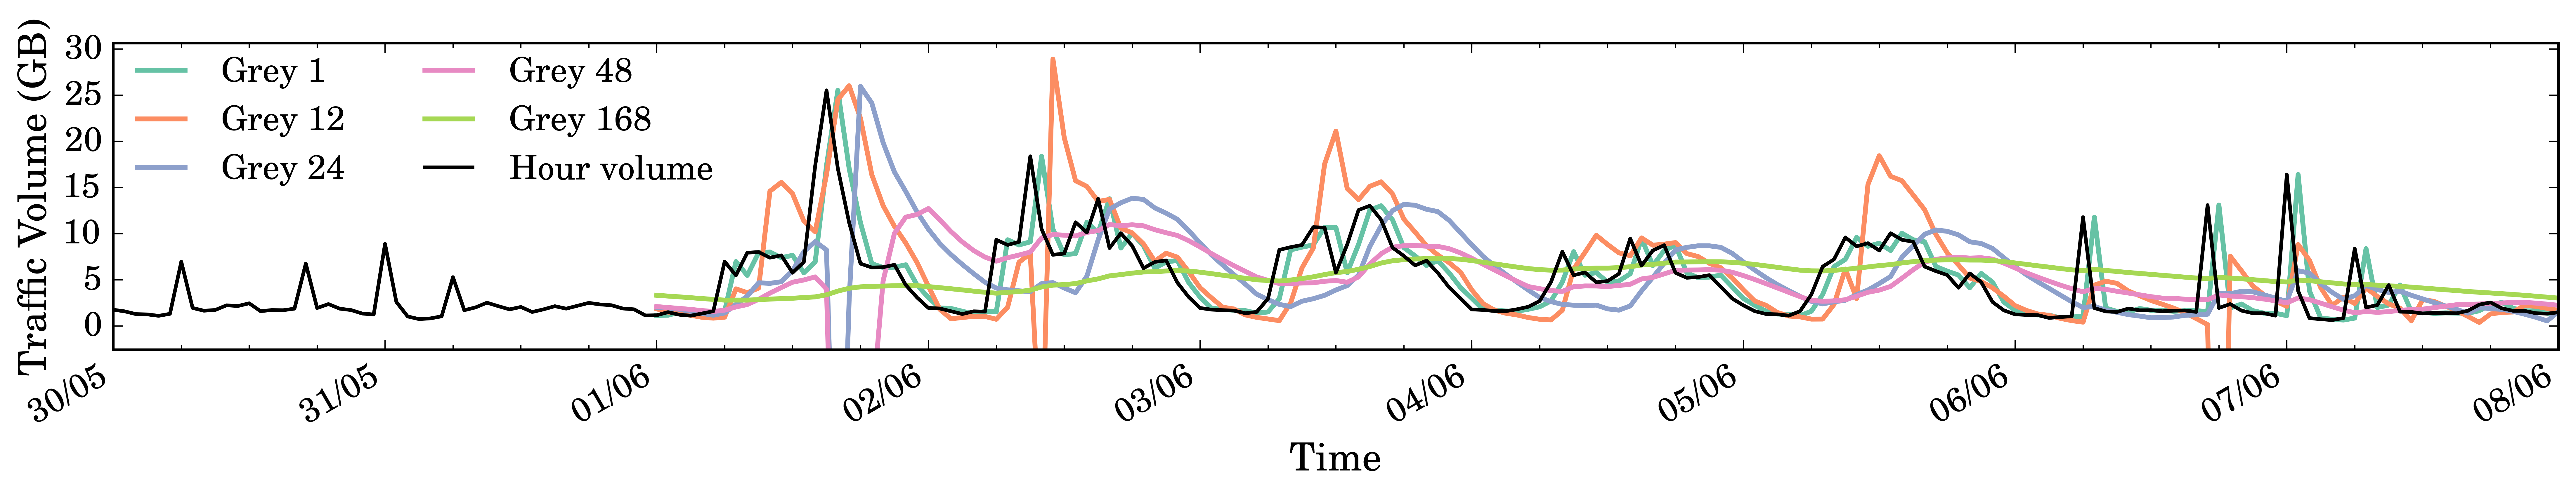
\includegraphics[width=\textwidth]{gfx/chap2/grey_sf.png}
                \caption{SF}
                \label{fig:grey_sf}
        \end{subfigure}
        \begin{subfigure}[b]{0.9\textwidth}
                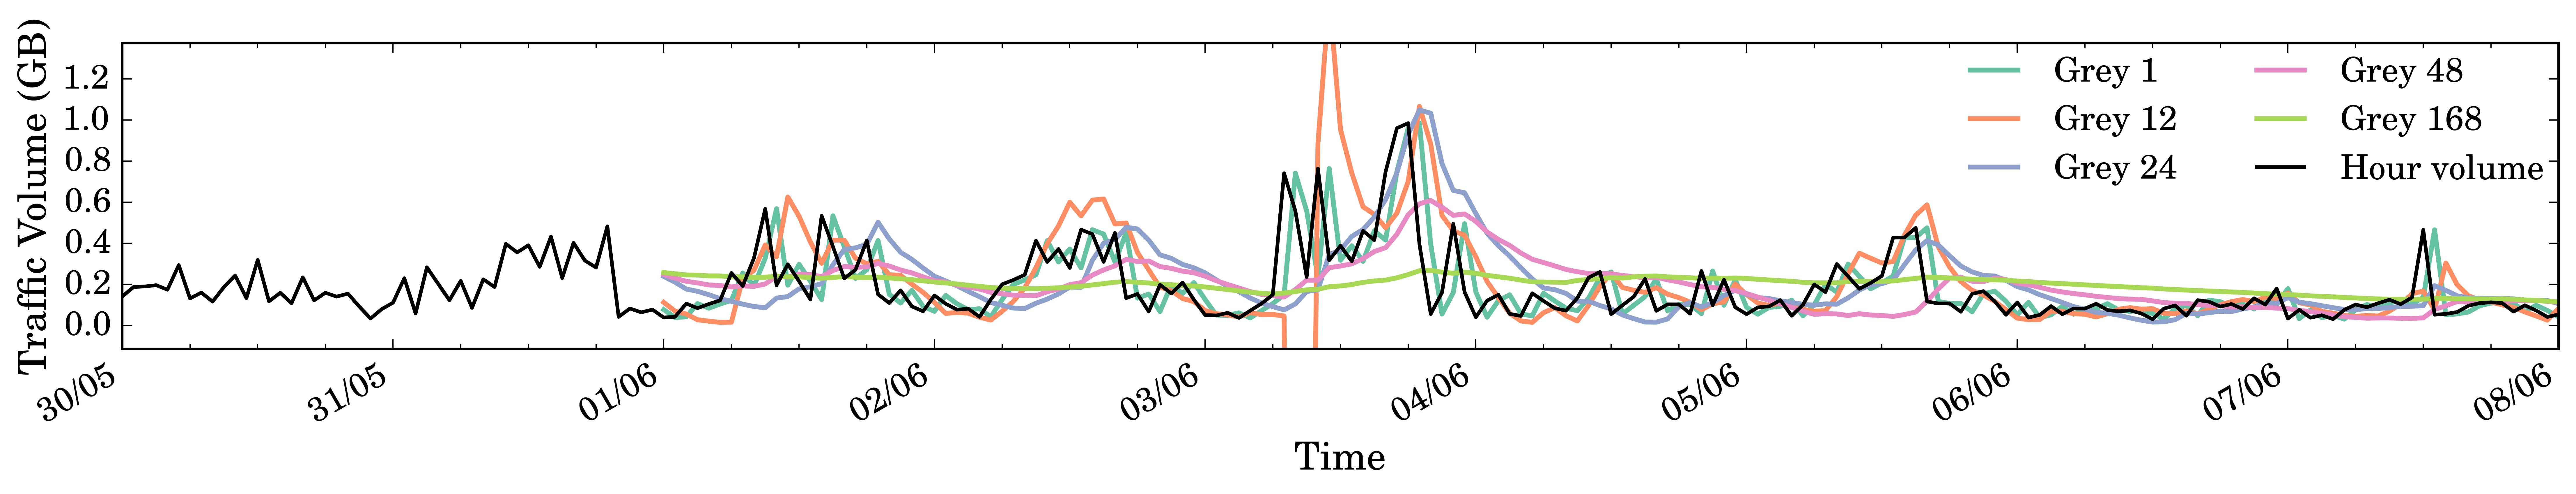
\includegraphics[width=\textwidth]{gfx/chap2/grey_sg.png}
                \caption{SG}
                \label{fig:grey_sg}
        \end{subfigure}
        \begin{subfigure}[b]{0.9\textwidth}
                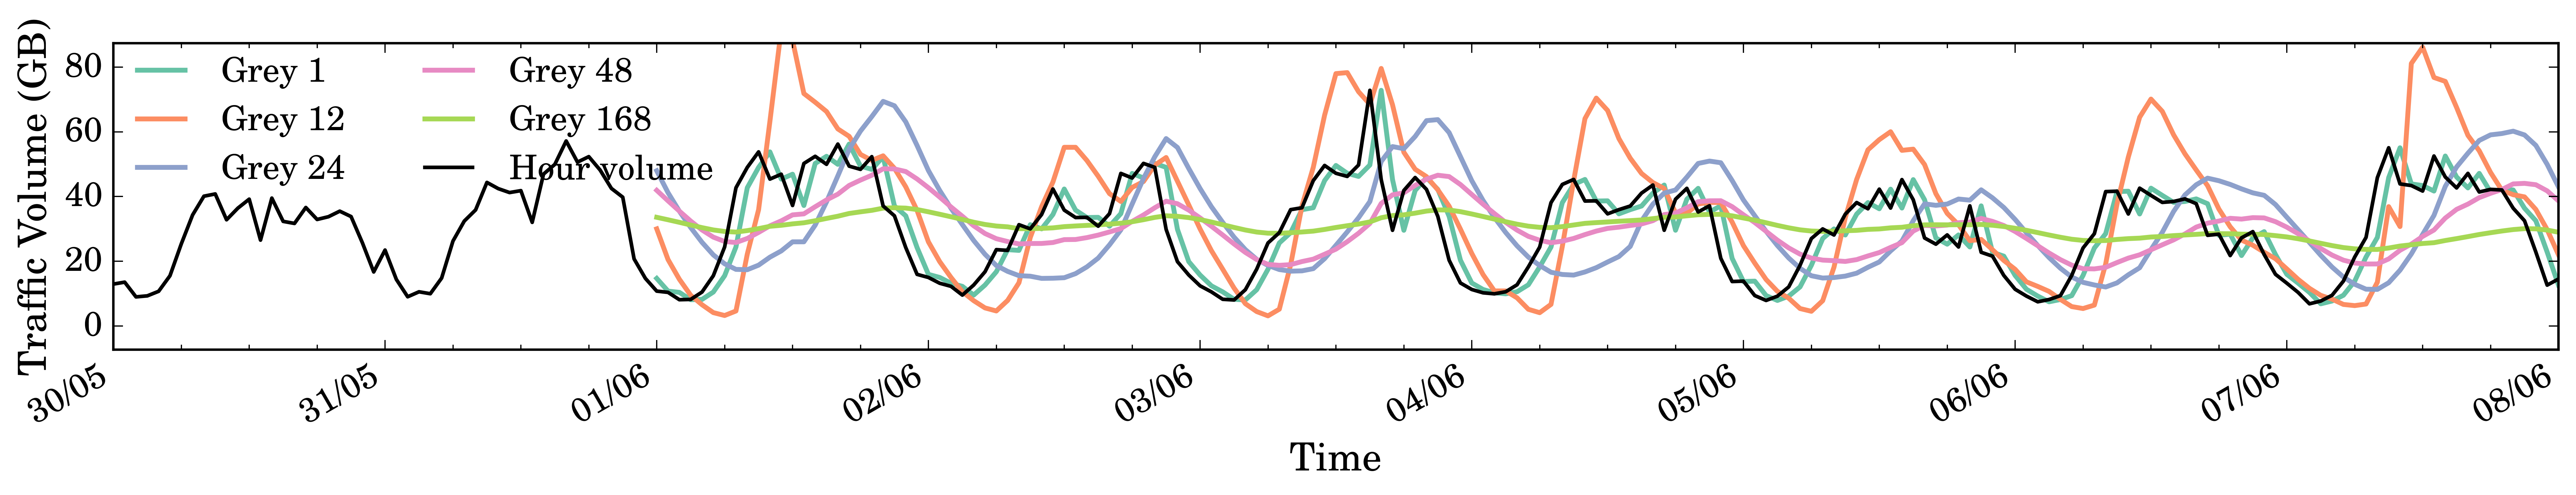
\includegraphics[width=\textwidth]{gfx/chap2/grey_sh.png}
                \caption{SH}
                \label{fig:grey_sh}
        \end{subfigure}
        \begin{subfigure}[b]{0.9\textwidth}
                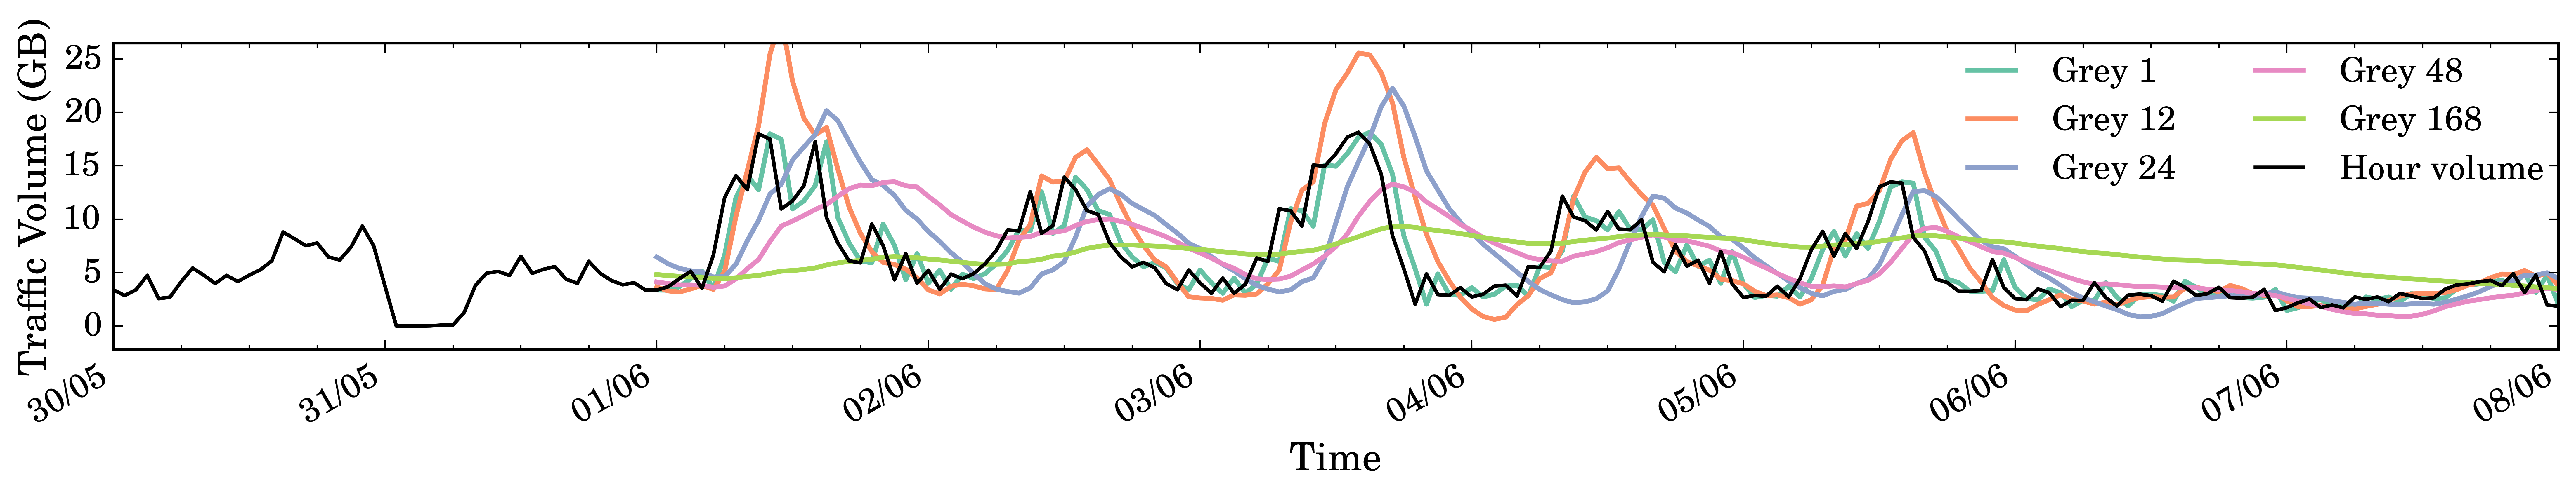
\includegraphics[width=\textwidth]{gfx/chap2/grey_si.png}
                \caption{SI}
                \label{fig:grey_si}
        \end{subfigure}
\caption{Predict total hour volume using $GM(1,1)$ with different historical record lengths for the week starting from June 1st, 2015.}
\label{fig:grey}
\end{figure}

\marginpar{Why grey model performs poorly?}
On the other hand, the hour volume coverage by grey model drops as we increase the historical records length and is in general much worse than the metrics proposed in this work. 
In order to understand the underlying reason, we used $GM(1,1)$ model described above to dynamically predict the total hour volume of all prefixes, which is normally much more regular and smoother than the volume series of individual prefixes, Fig.~\ref{fig:grey}.

\marginpar{overreact to sudden value change.}
For site SB and SD, we miss the hour volume data for the week starting from May 25th. 
$GM(1,1)$ model using records of last $168$ suffer a lot from  data missing, normal volume sequences by 0s,  and converge extremely slow to values in reasonable range. 
However, such sudden change in value is not unexpected, since bursty prefixes can bring huge amount of traffic within in a short duration and then remain silent over days. Such prefixes are commonly seen on SC, SF, SG judging from their burstiness index in Table~\ref{tab:bi}.
This explains why grey model leads to fairly low volume coverage in Fig.~\ref{fig:cvg_sc}. 

\marginpar{delayed response to value change}
Furthermore, in Fig.~\ref{fig:grey_sb}, Fig.~\ref{fig:grey_sc} and as well in others, we can see that grey model reacts to volume variations in a delayed manner. Longer the historical records length is, more obvious and longer grey model delays the variations of actual trace.  
This behavior could be fatal in the presence of bursty prefixes.
We can observe considerably large pikes in both directions several hours after the volume burst in Fig.~\ref{fig:grey_sc}, which might greatly disturb the prefix selection during those periods and consequently give rise to low volume coverage.

Compared to grey model, metrics proposed in our work do not directly predict hour volumes of each prefix but rather are indirect measures of prefix volume importance. And analysis in Section~\ref{sec:dyna} showed that the overall coverage using these metrics are guaranteed by the traffic character itself.

\begin{figure}
\centering
		\centering
        \begin{subfigure}[b]{0.48\textwidth}
                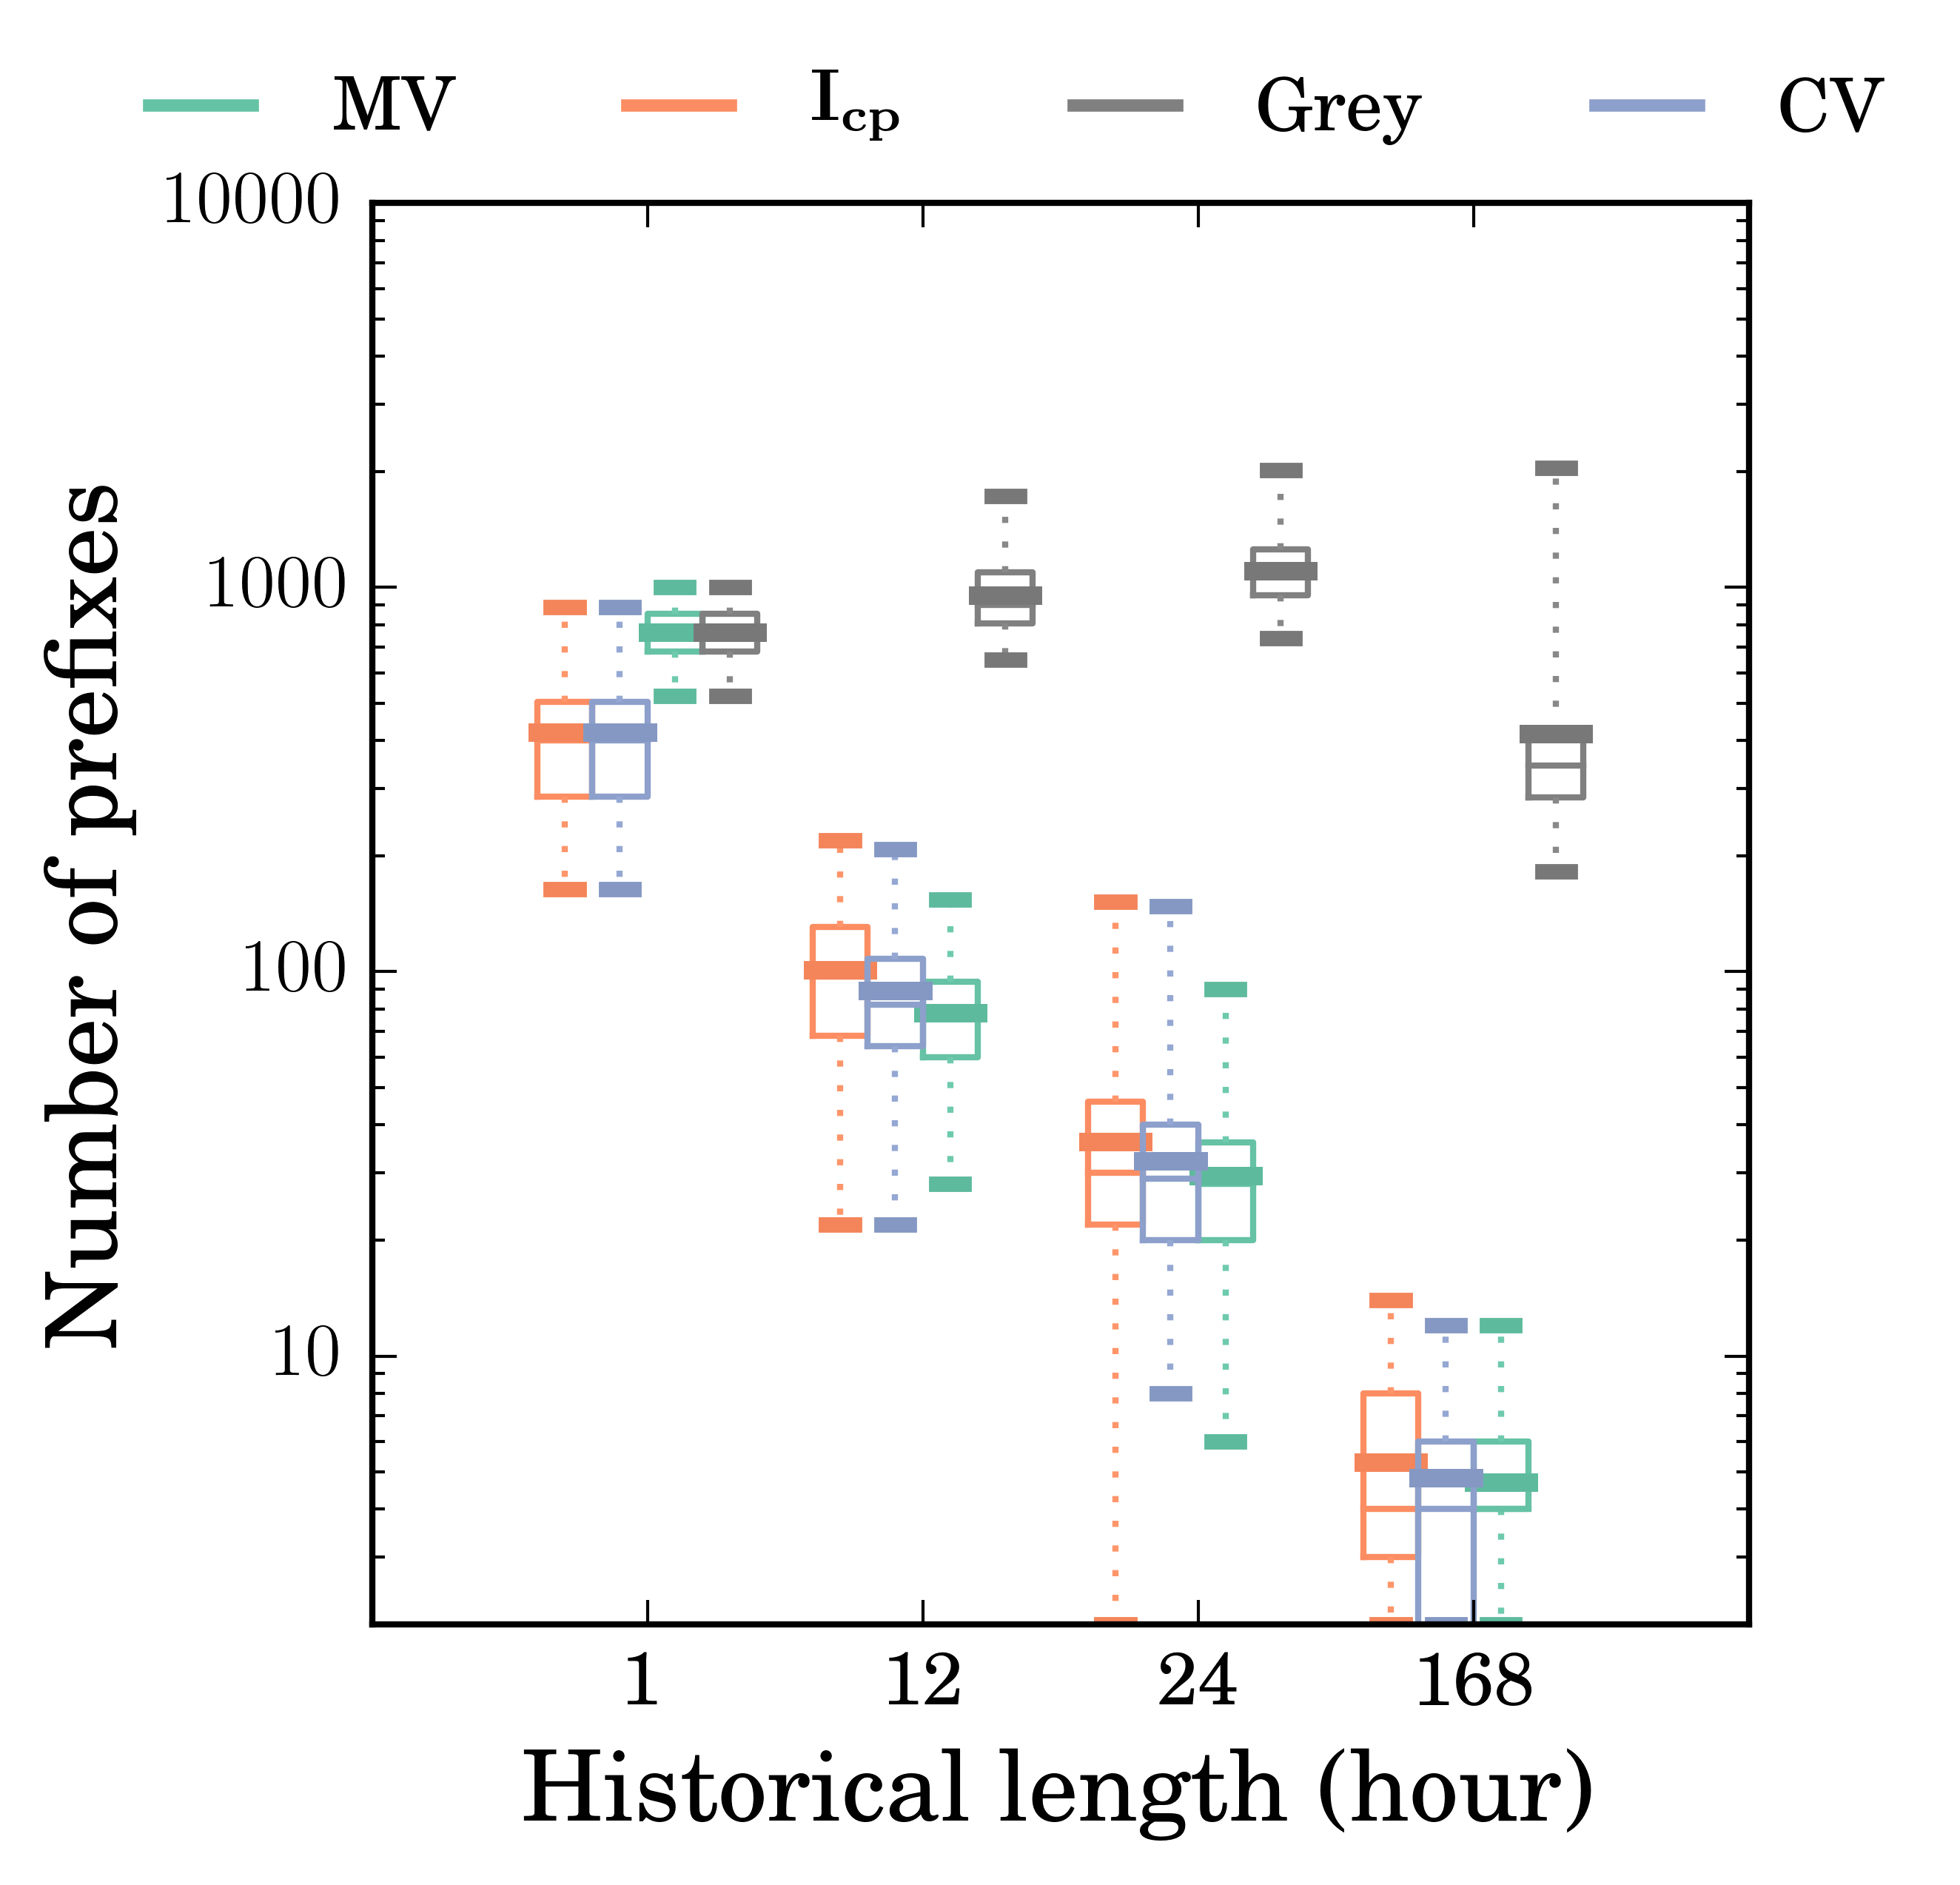
\includegraphics[width=\textwidth]{gfx/chap2/grey_churn_box_method_compare_fs_sa.png}
                \caption{SA}
                \label{fig:churn_sa}
        \end{subfigure}
        \begin{subfigure}[b]{0.48\textwidth}
                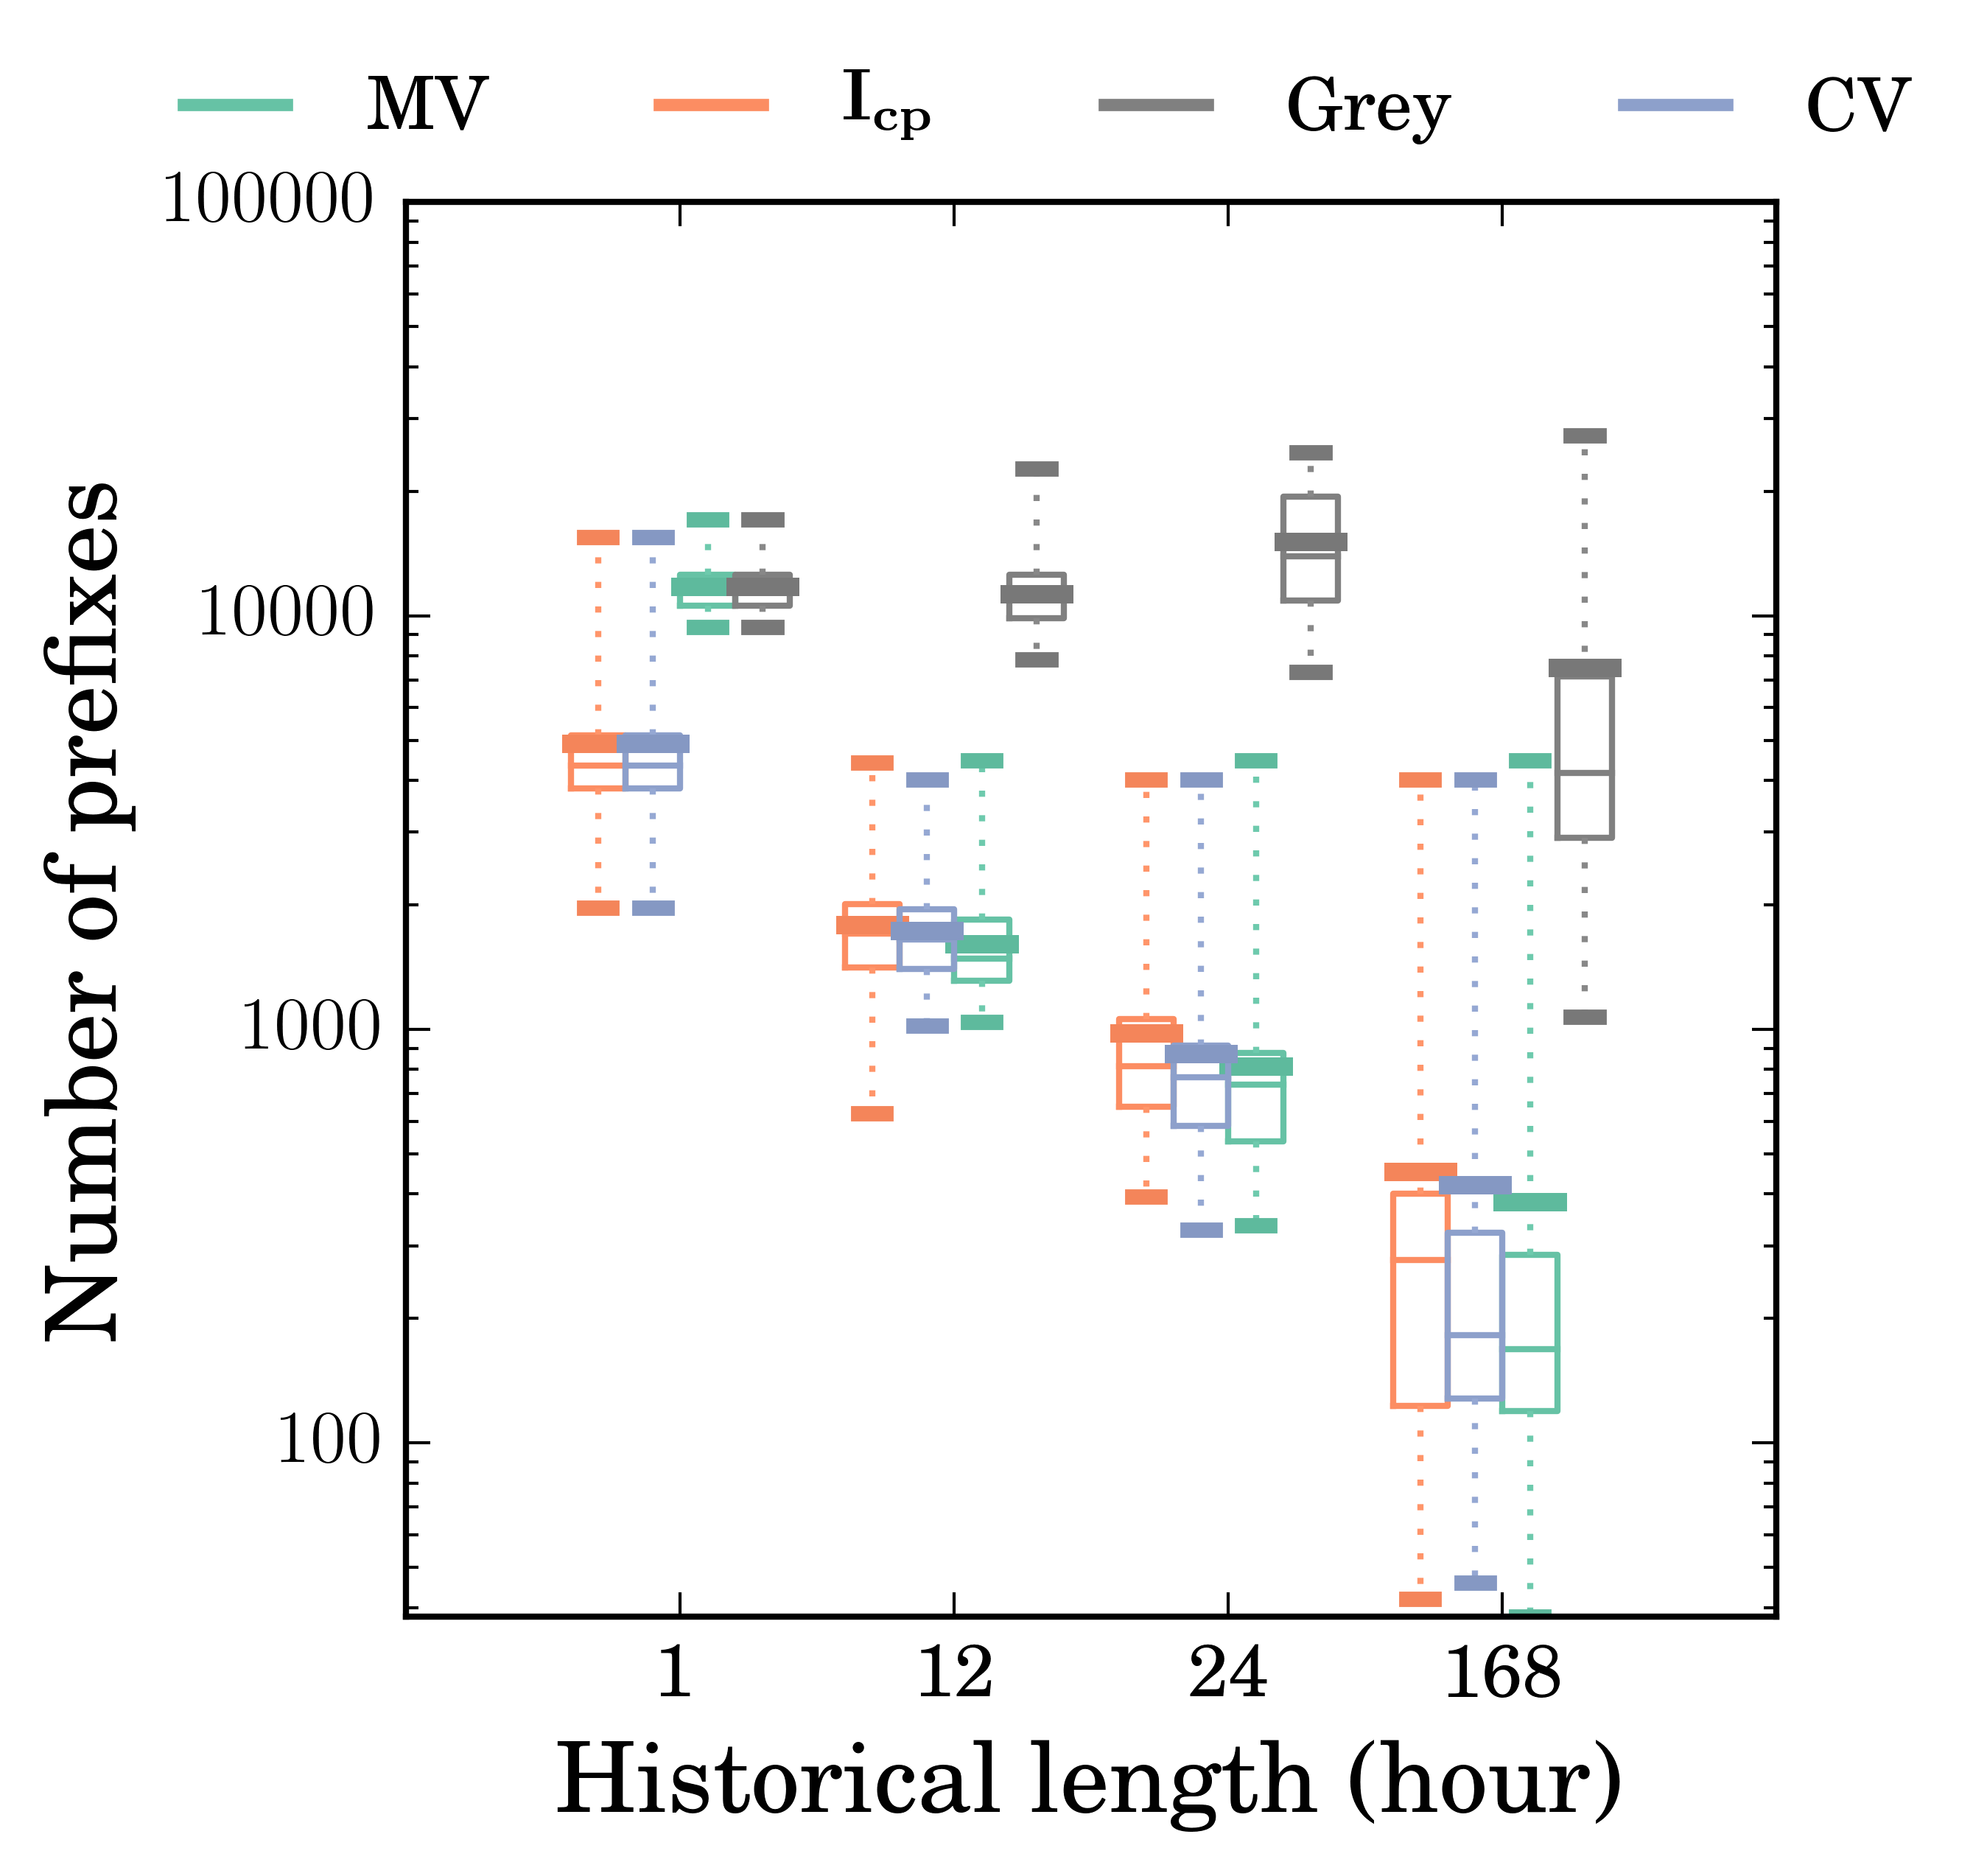
\includegraphics[width=\textwidth]{gfx/chap2/grey_churn_box_method_compare_fs_sb.png}
                \caption{SB}
                \label{fig:churn_sb}
        \end{subfigure}
        \begin{subfigure}[b]{0.48\textwidth}
                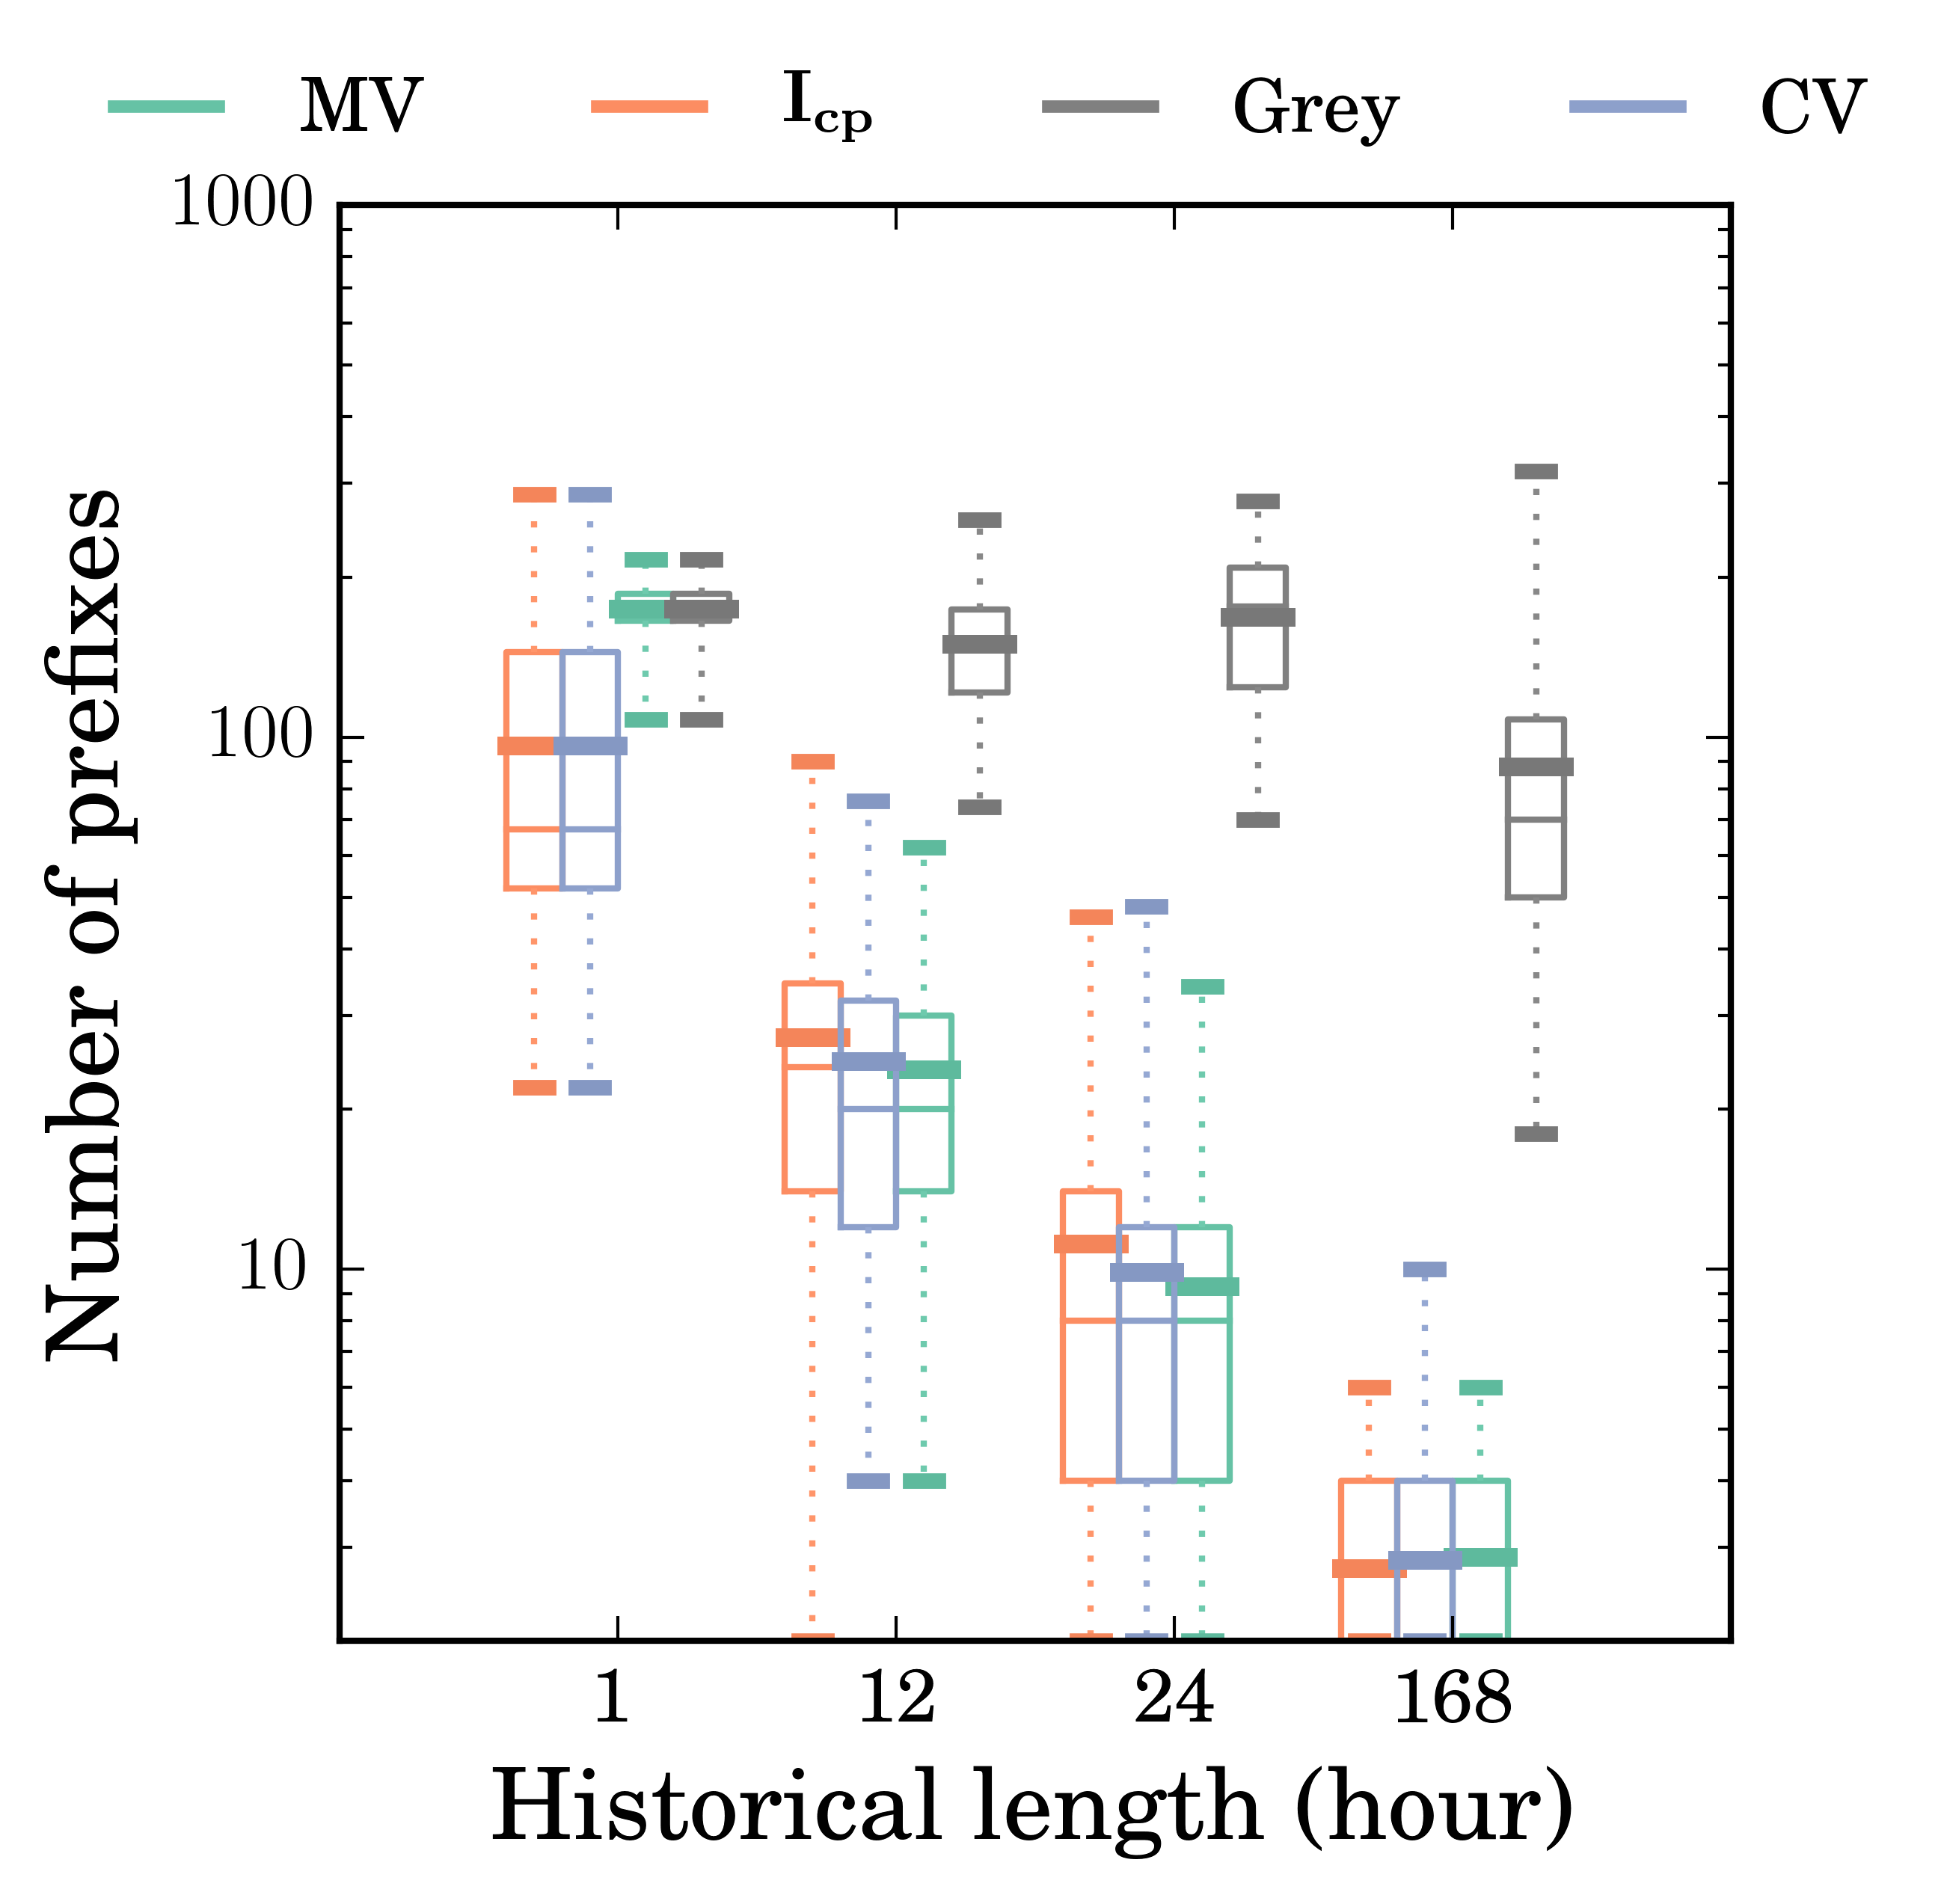
\includegraphics[width=\textwidth]{gfx/chap2/grey_churn_box_method_compare_fs_sc.png}
                \caption{SC}
                \label{fig:churn_sc}
        \end{subfigure}
        \begin{subfigure}[b]{0.48\textwidth}
                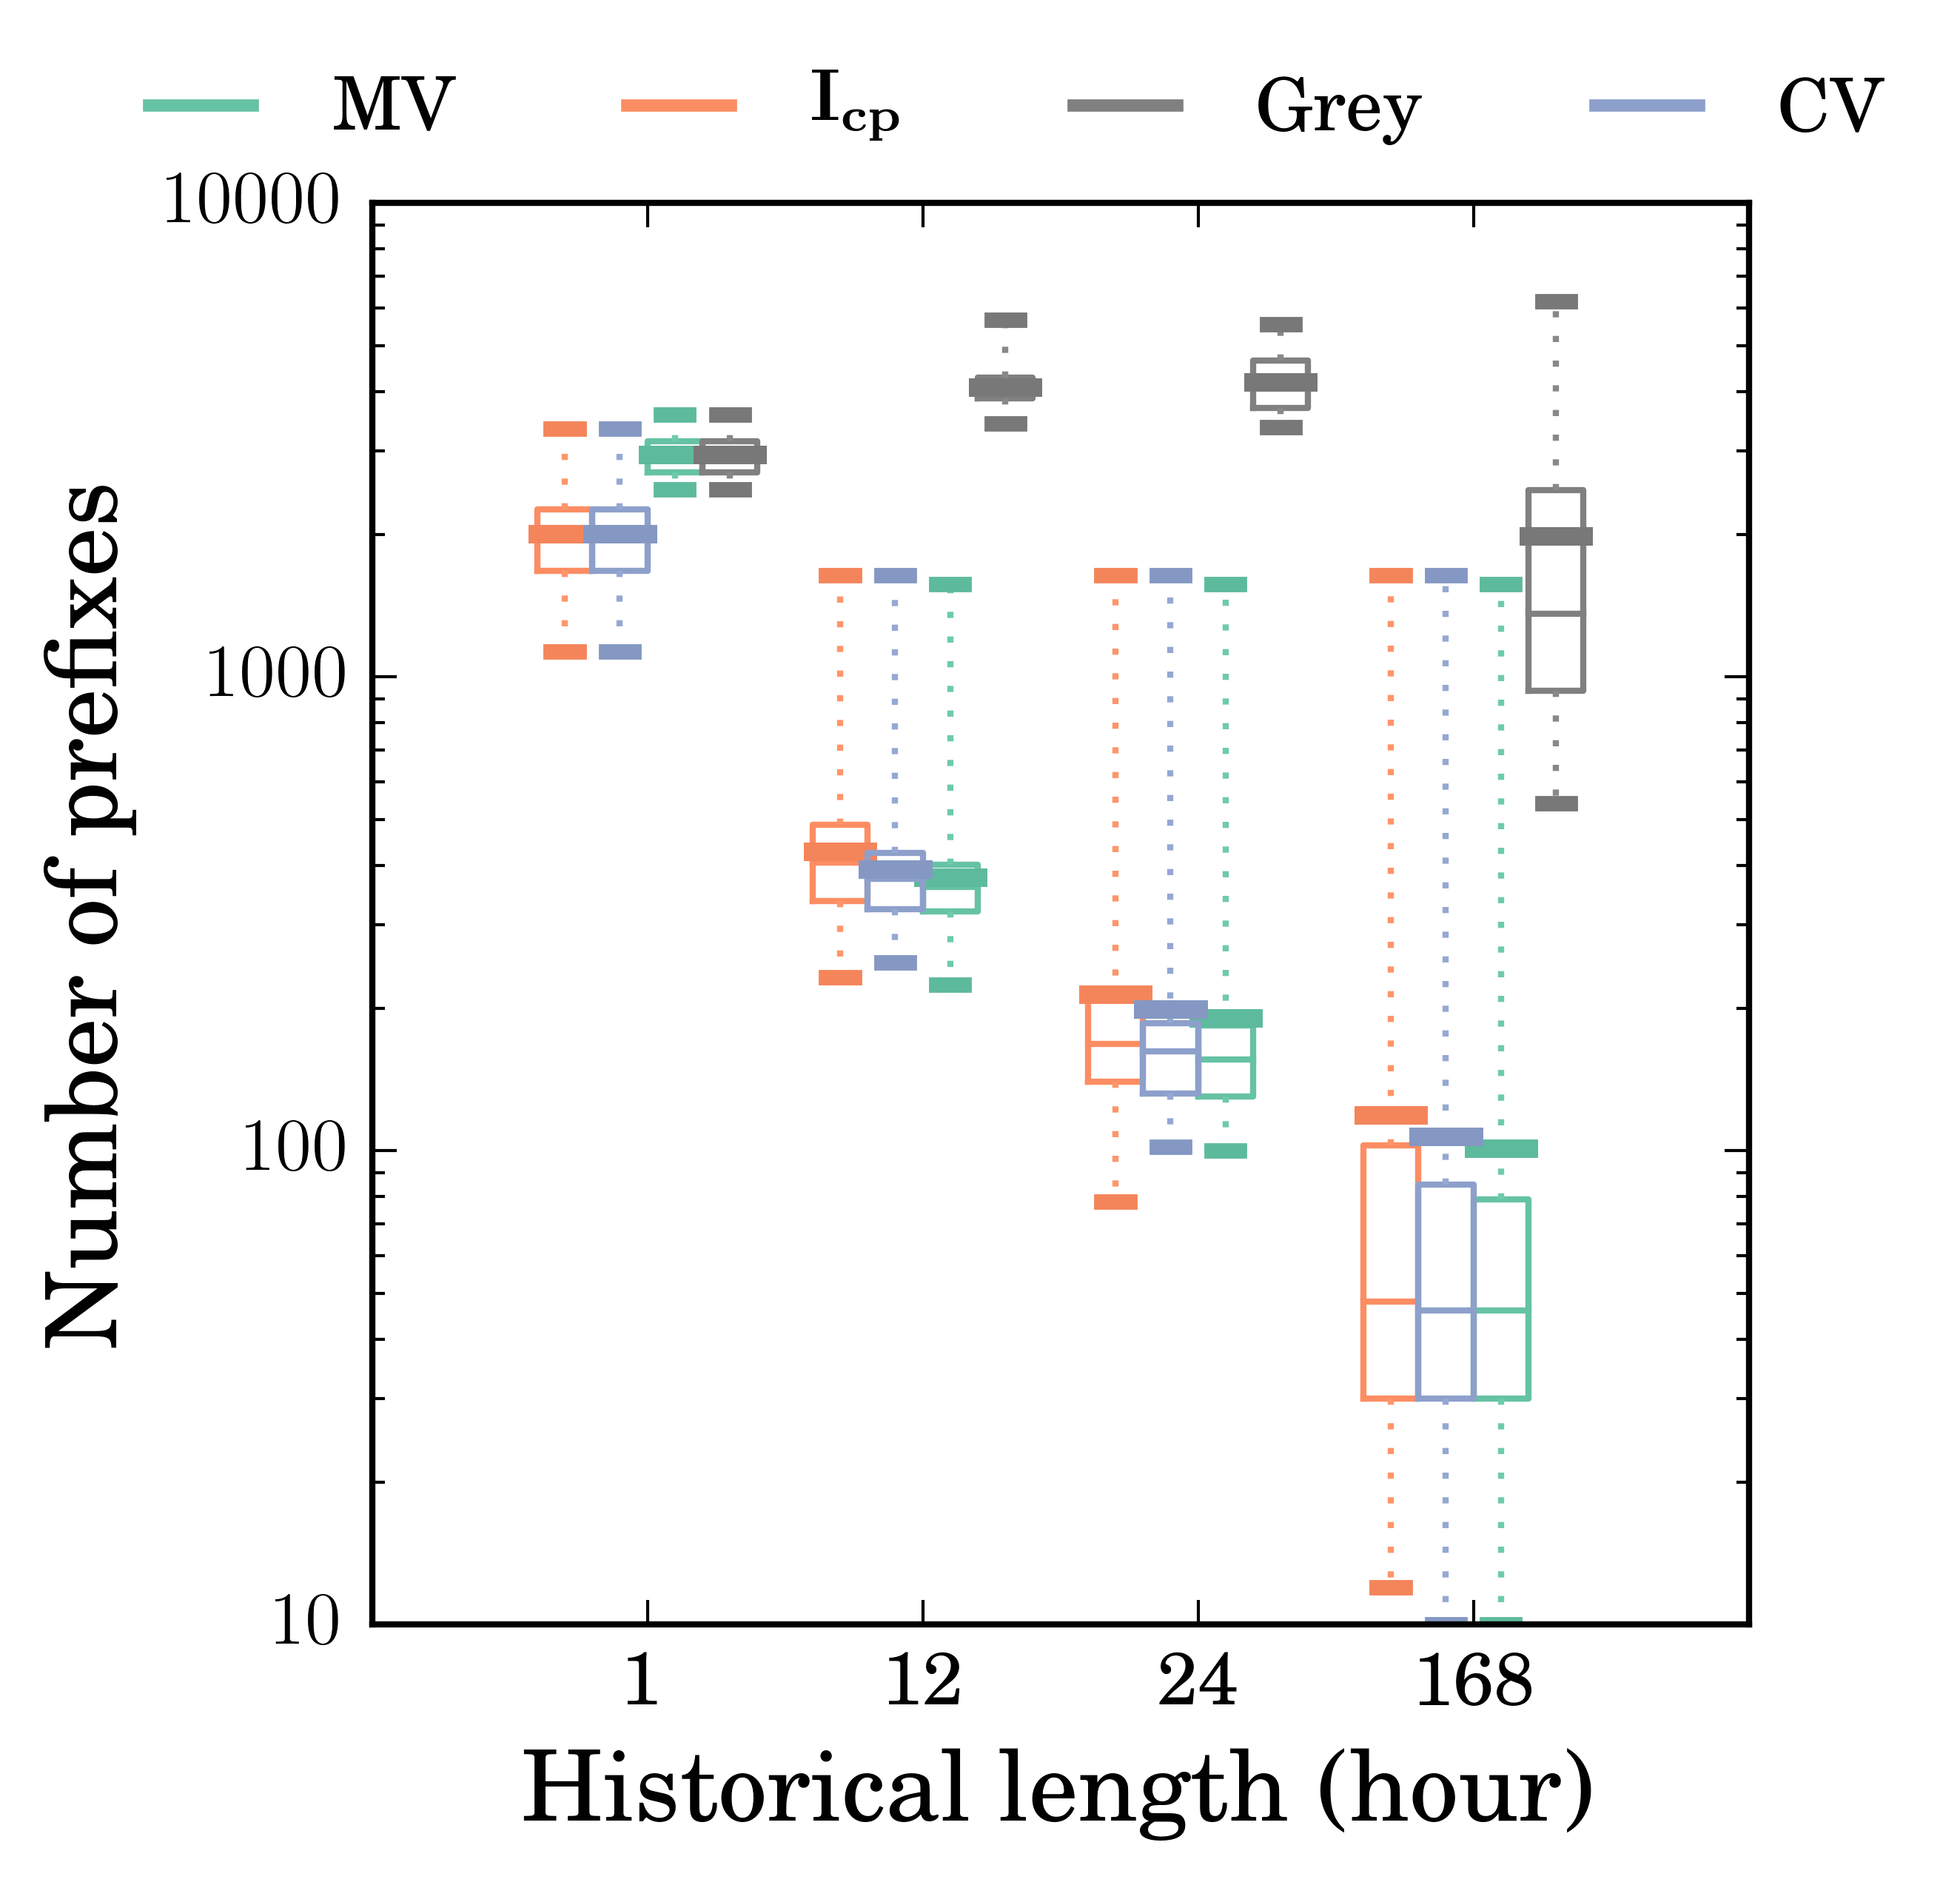
\includegraphics[width=\textwidth]{gfx/chap2/grey_churn_box_method_compare_fs_sd.png}
                \caption{SD}
                \label{fig:churn_sd}
        \end{subfigure}
        \begin{subfigure}[b]{0.48\textwidth}
                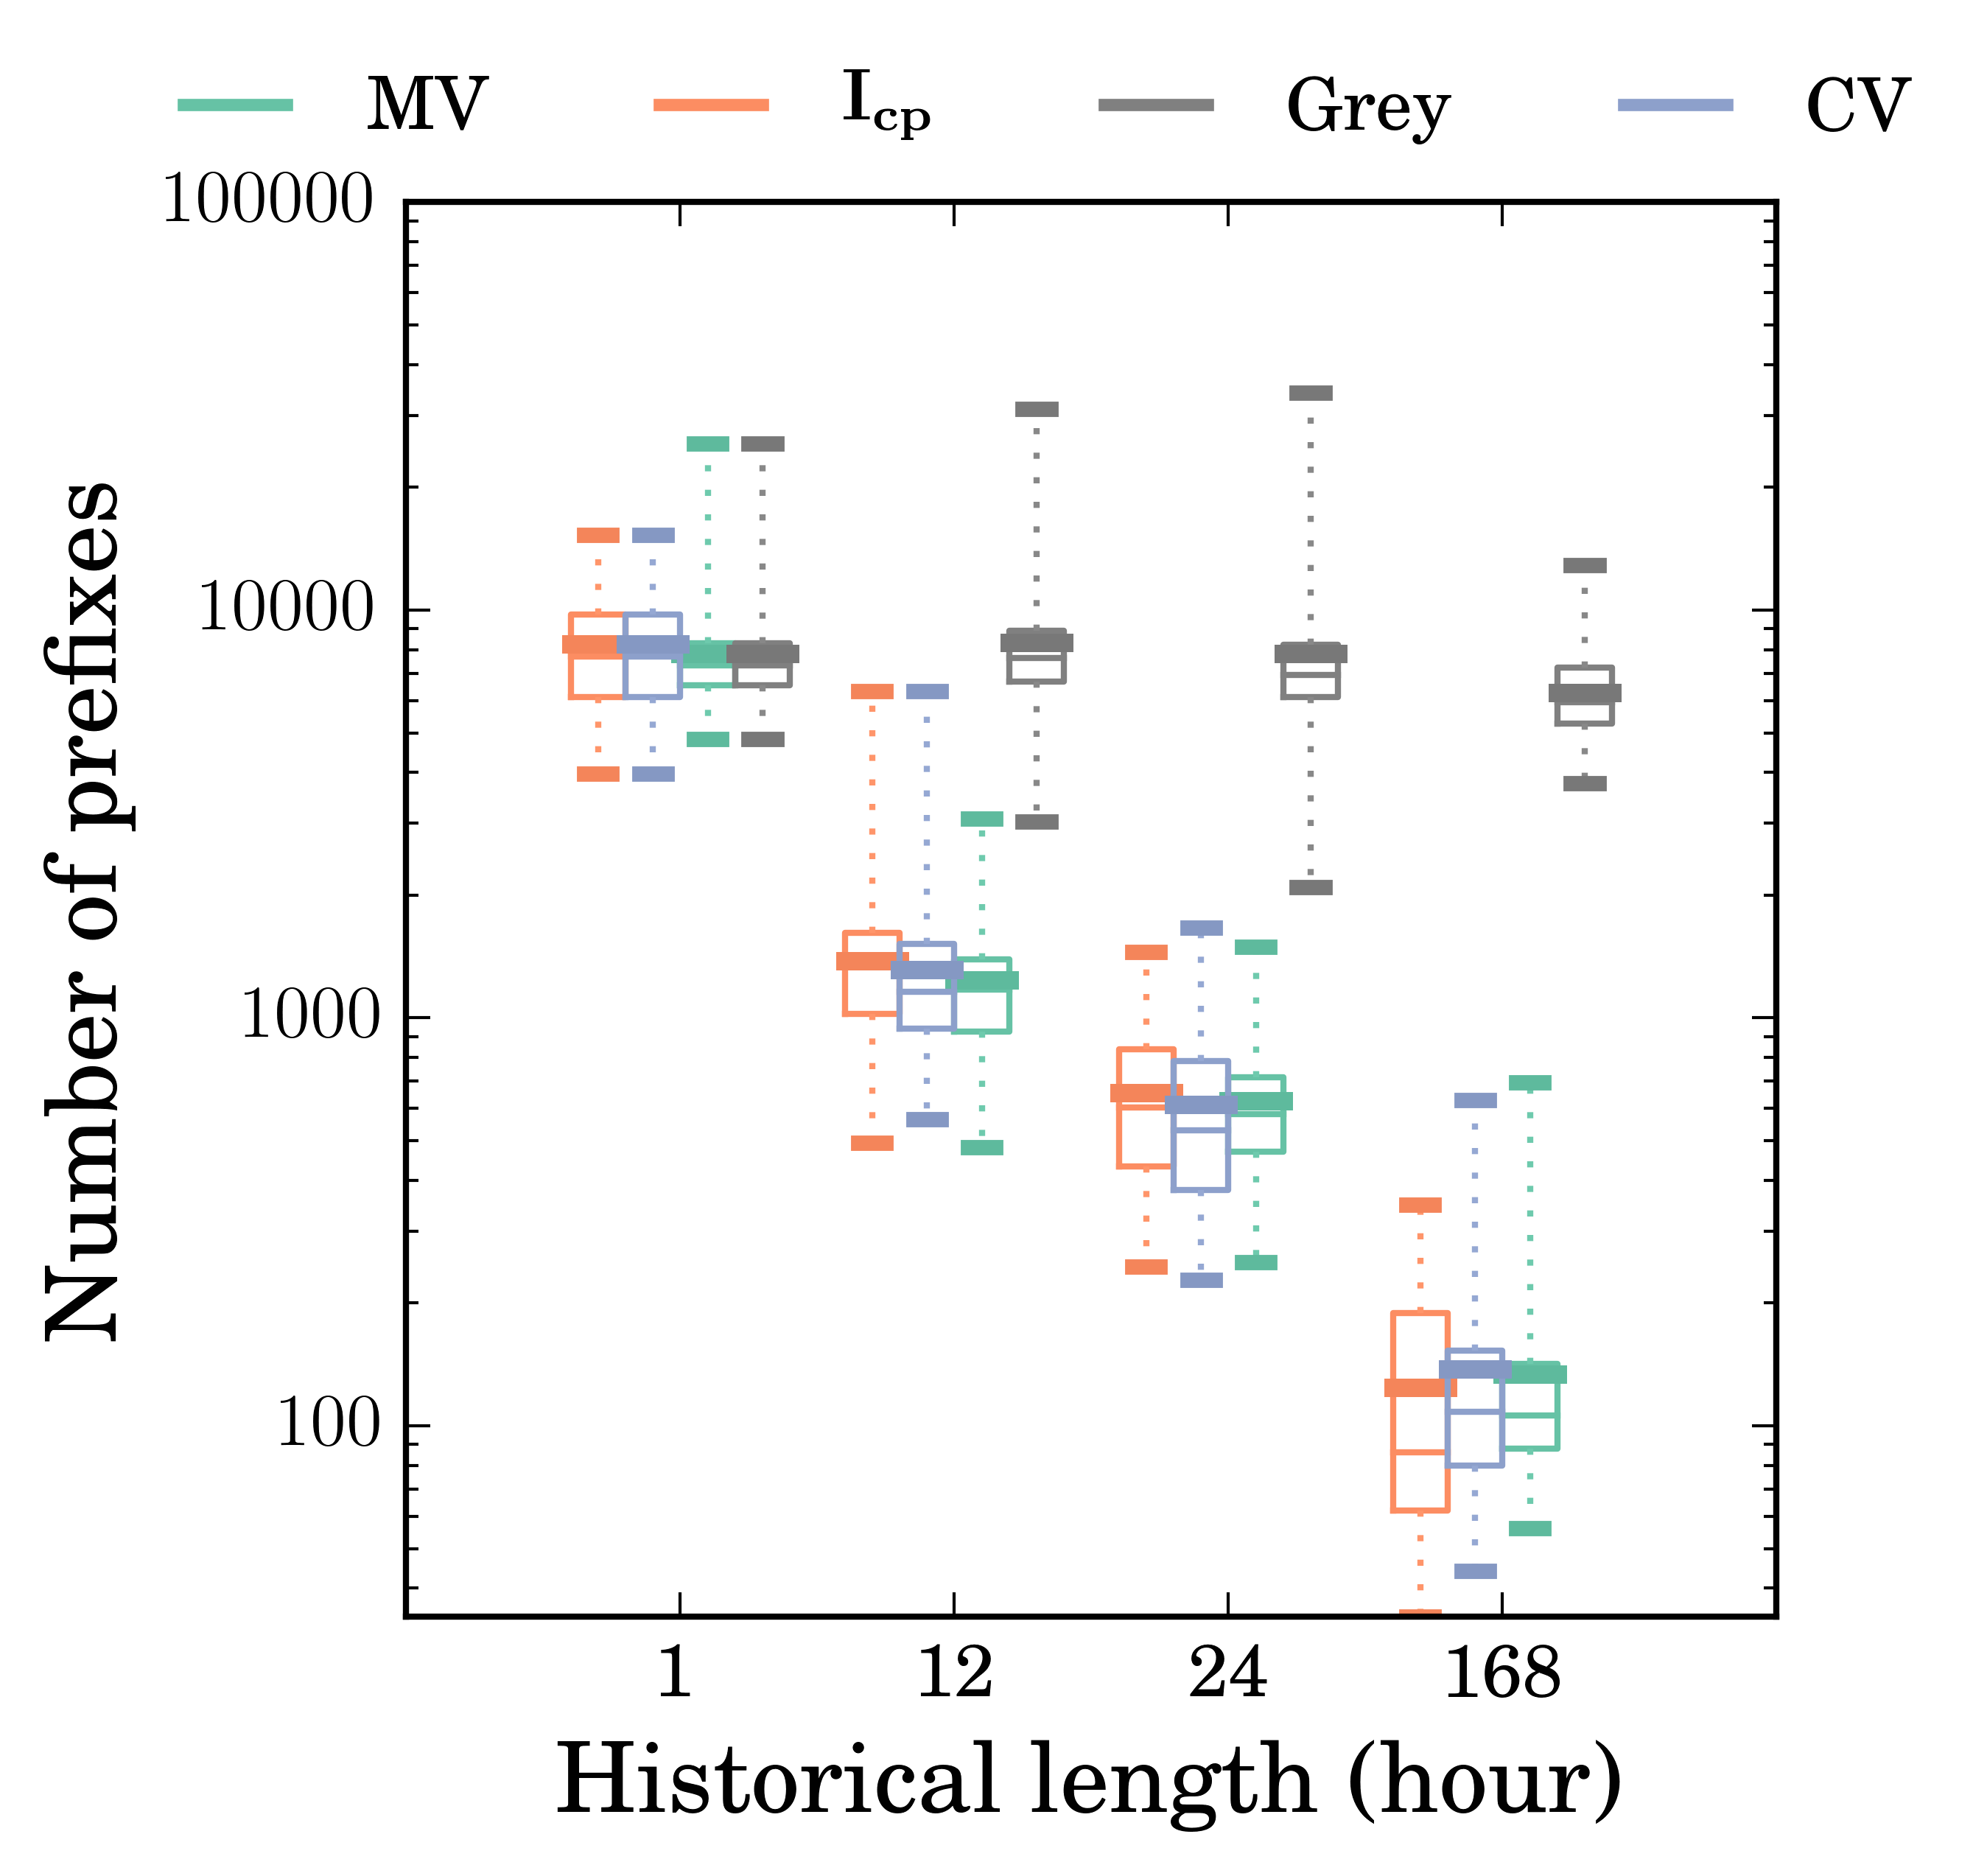
\includegraphics[width=\textwidth]{gfx/chap2/grey_churn_box_method_compare_fs_se.png}
                \caption{SE}
                \label{fig:churn_se}
        \end{subfigure}
        \begin{subfigure}[b]{0.48\textwidth}
                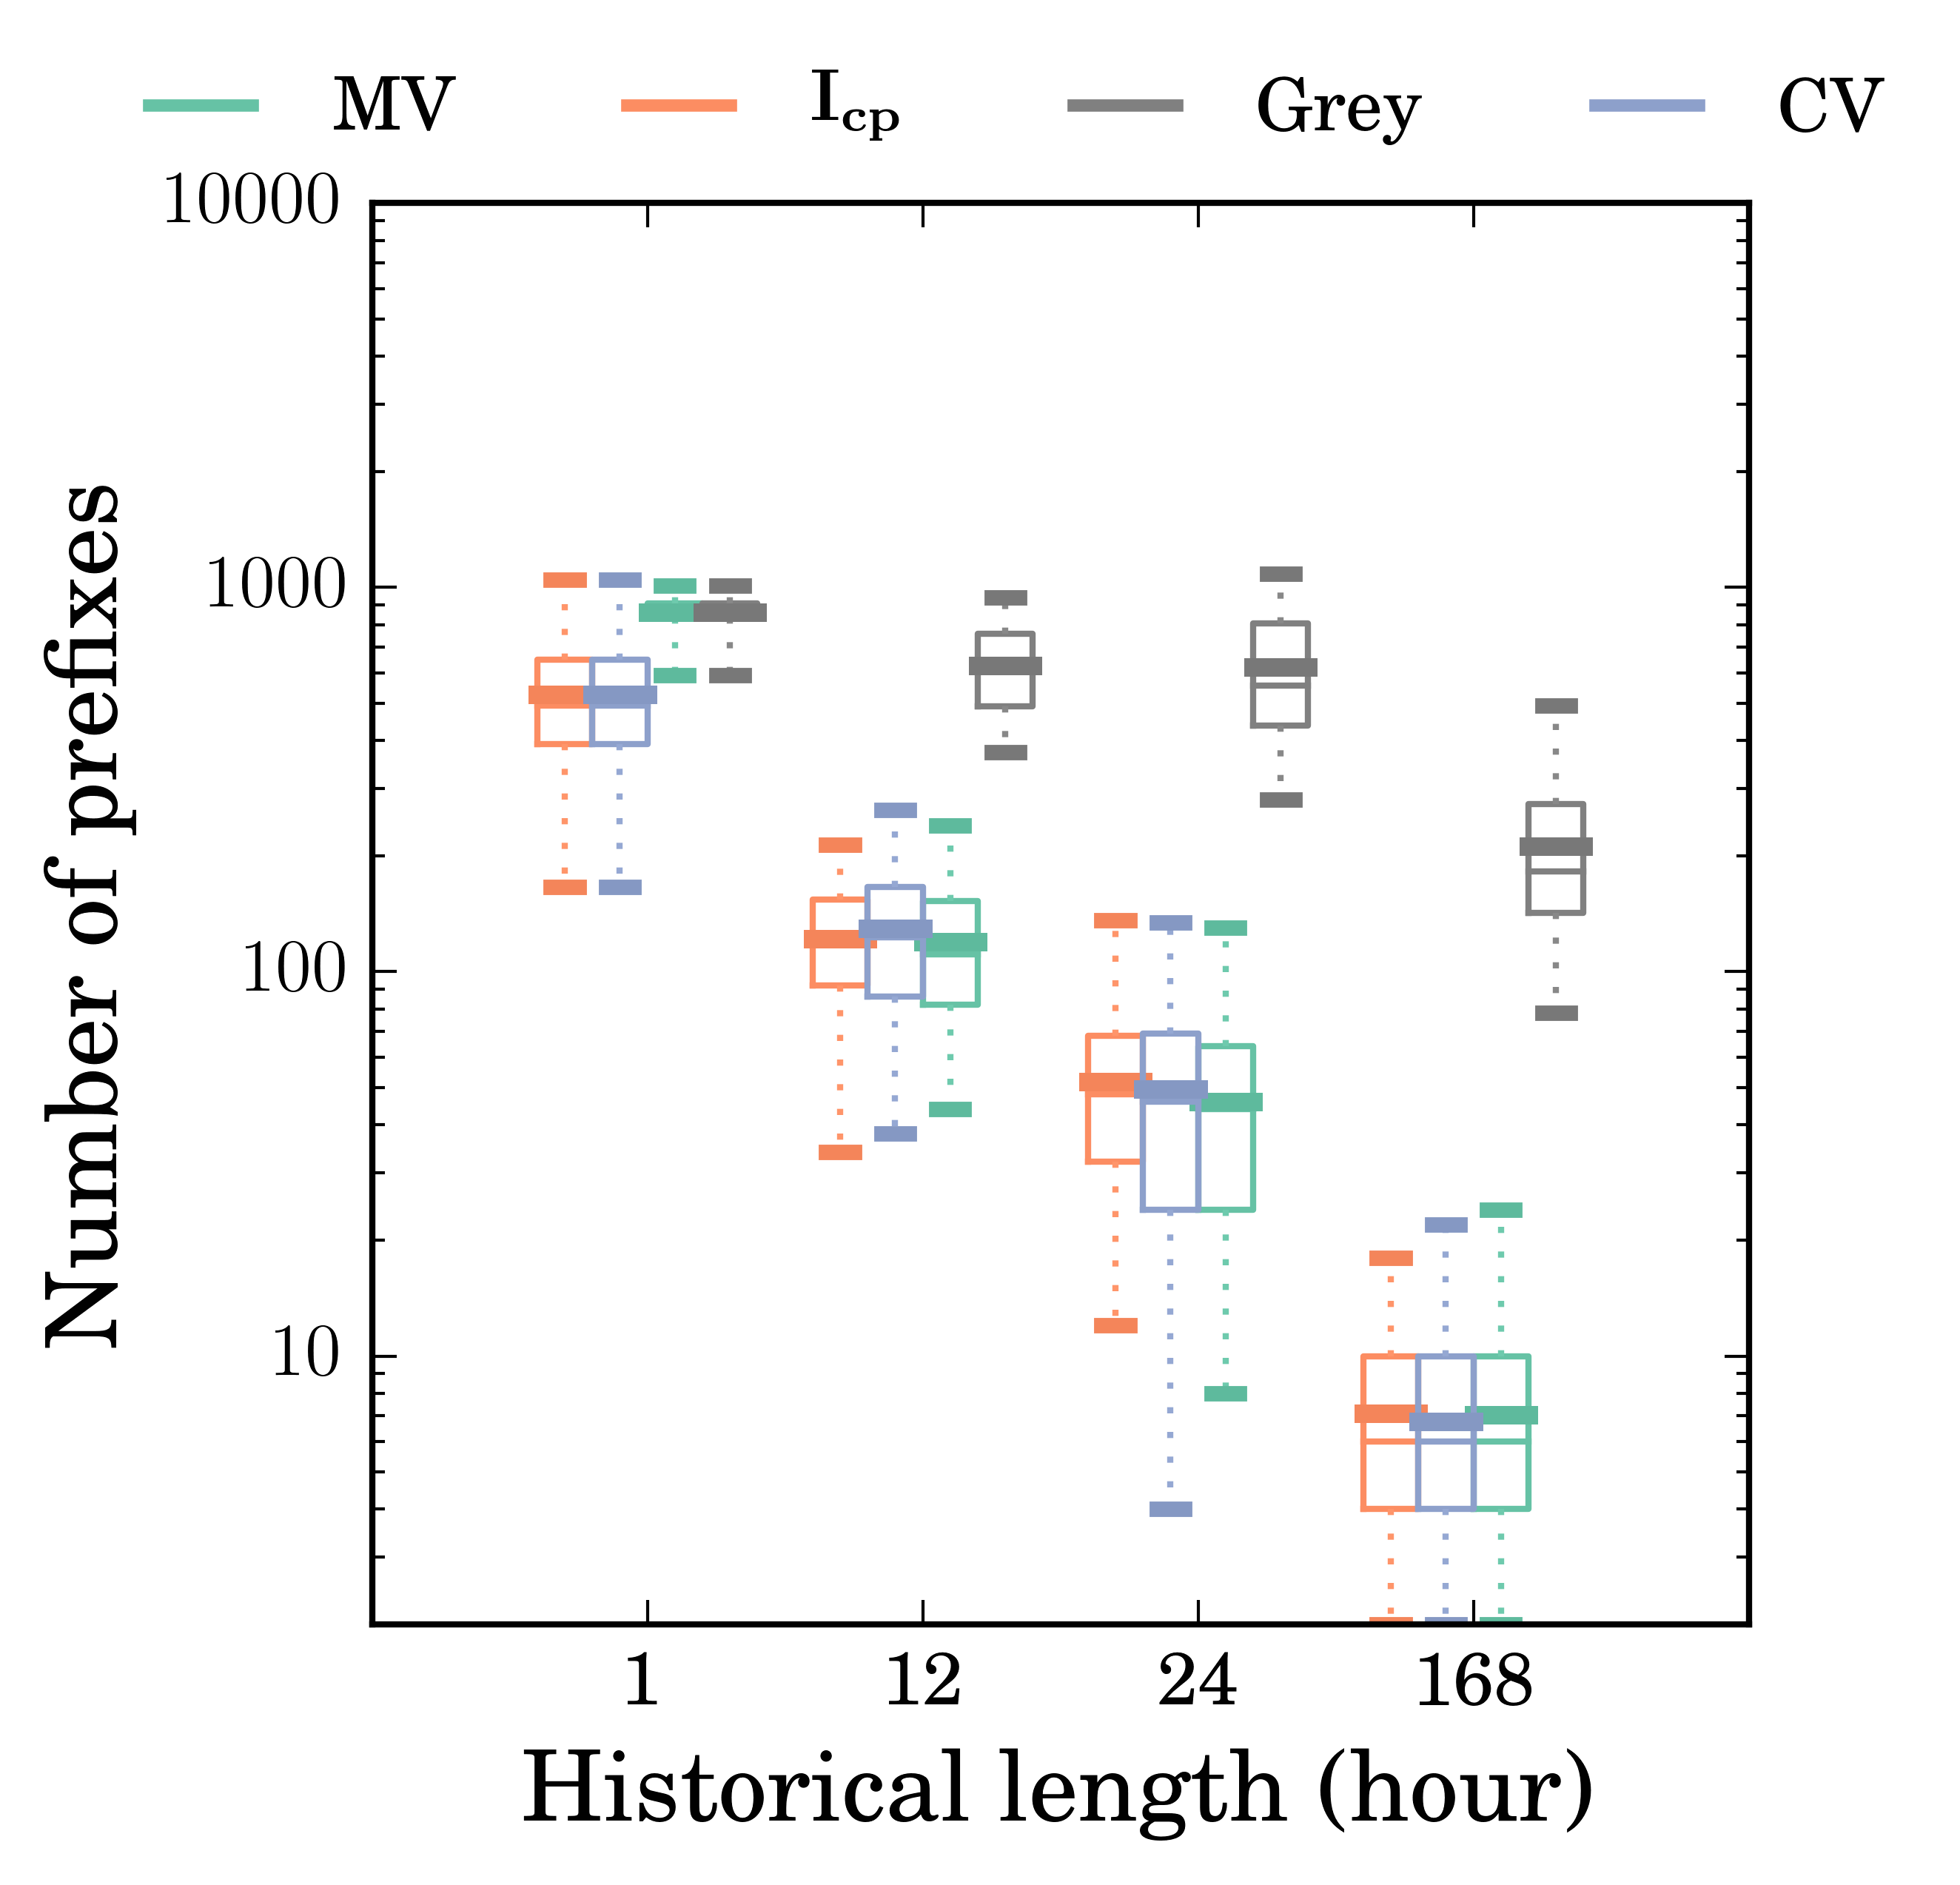
\includegraphics[width=\textwidth]{gfx/chap2/grey_churn_box_method_compare_fs_sf.png}
                \caption{SF}
                \label{fig:churn_sf}
        \end{subfigure}
\caption{Hour churn of the prefix set predictively selected using historical records of different lengths. The selection set size of each network is set to the maximum \textit{core} size over the week starting from June 1st, 2015, see in Table~\ref{tab:core_size}.}
\label{fig:churn}
\end{figure}

\begin{figure}\ContinuedFloat 
        \begin{subfigure}[b]{0.48\textwidth}
                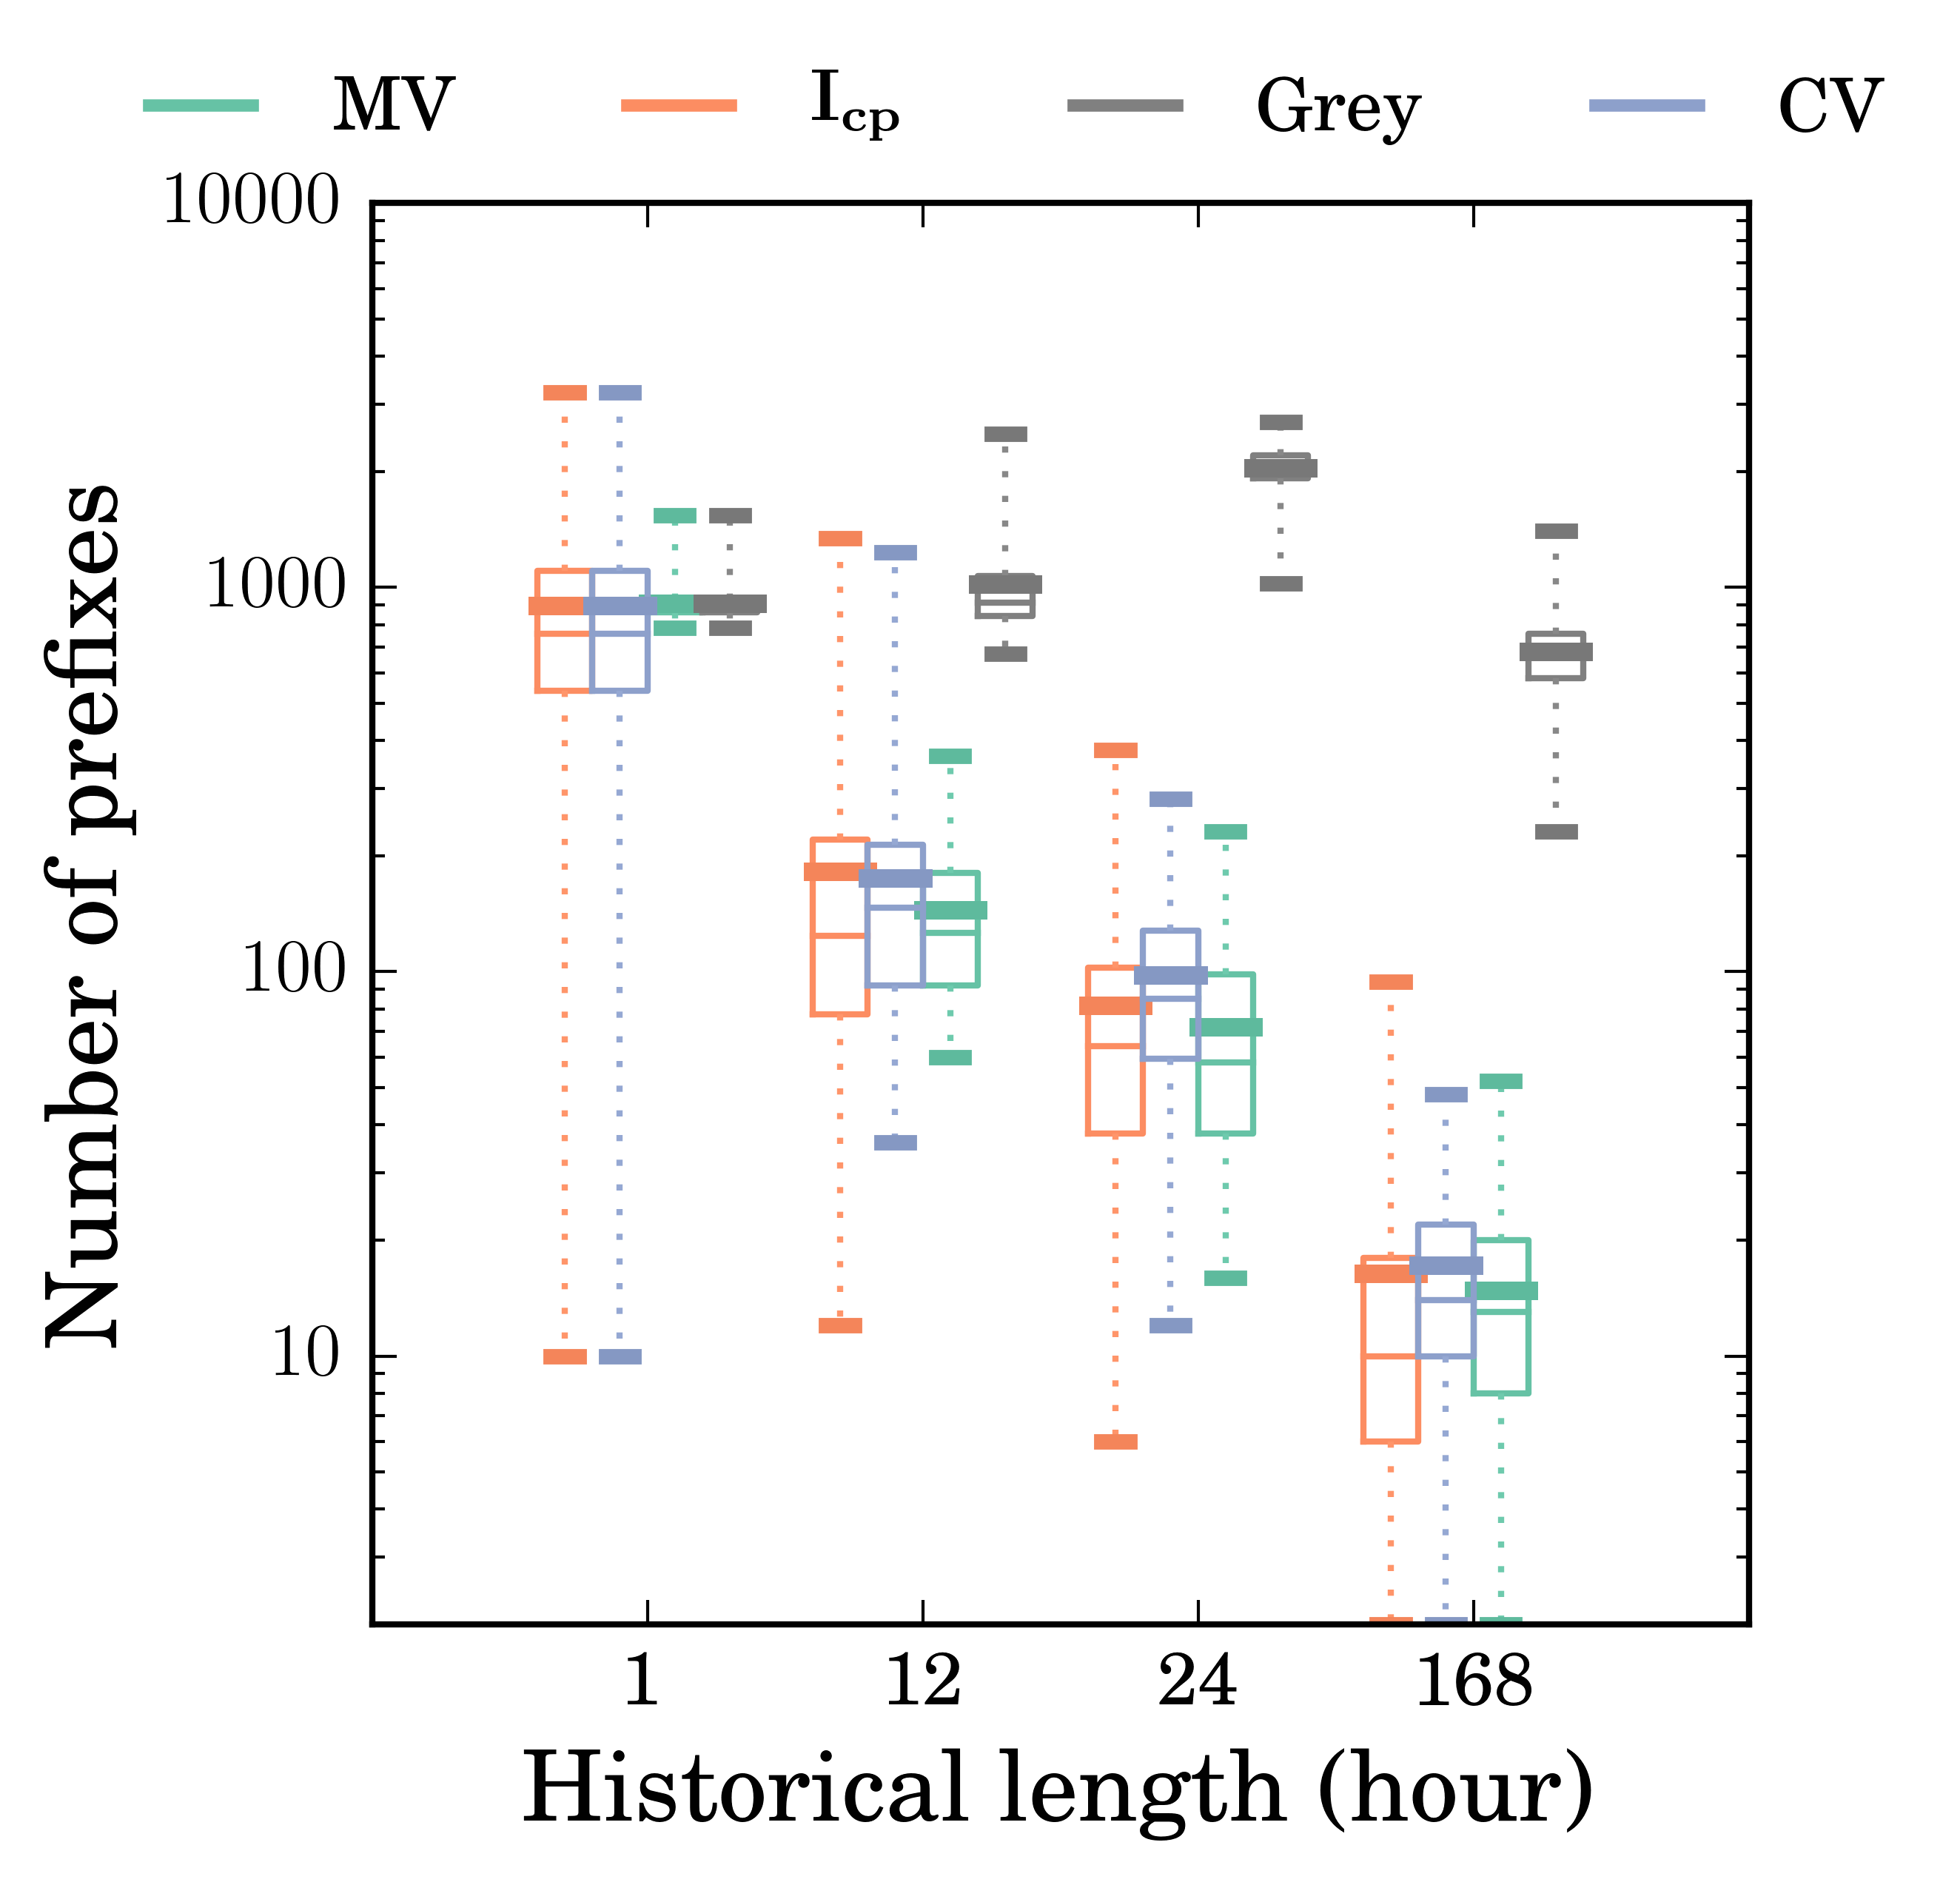
\includegraphics[width=\textwidth]{gfx/chap2/grey_churn_box_method_compare_fs_sg.png}
                \caption{SG}
                \label{fig:churn_sg}
        \end{subfigure}
        \begin{subfigure}[b]{0.48\textwidth}
                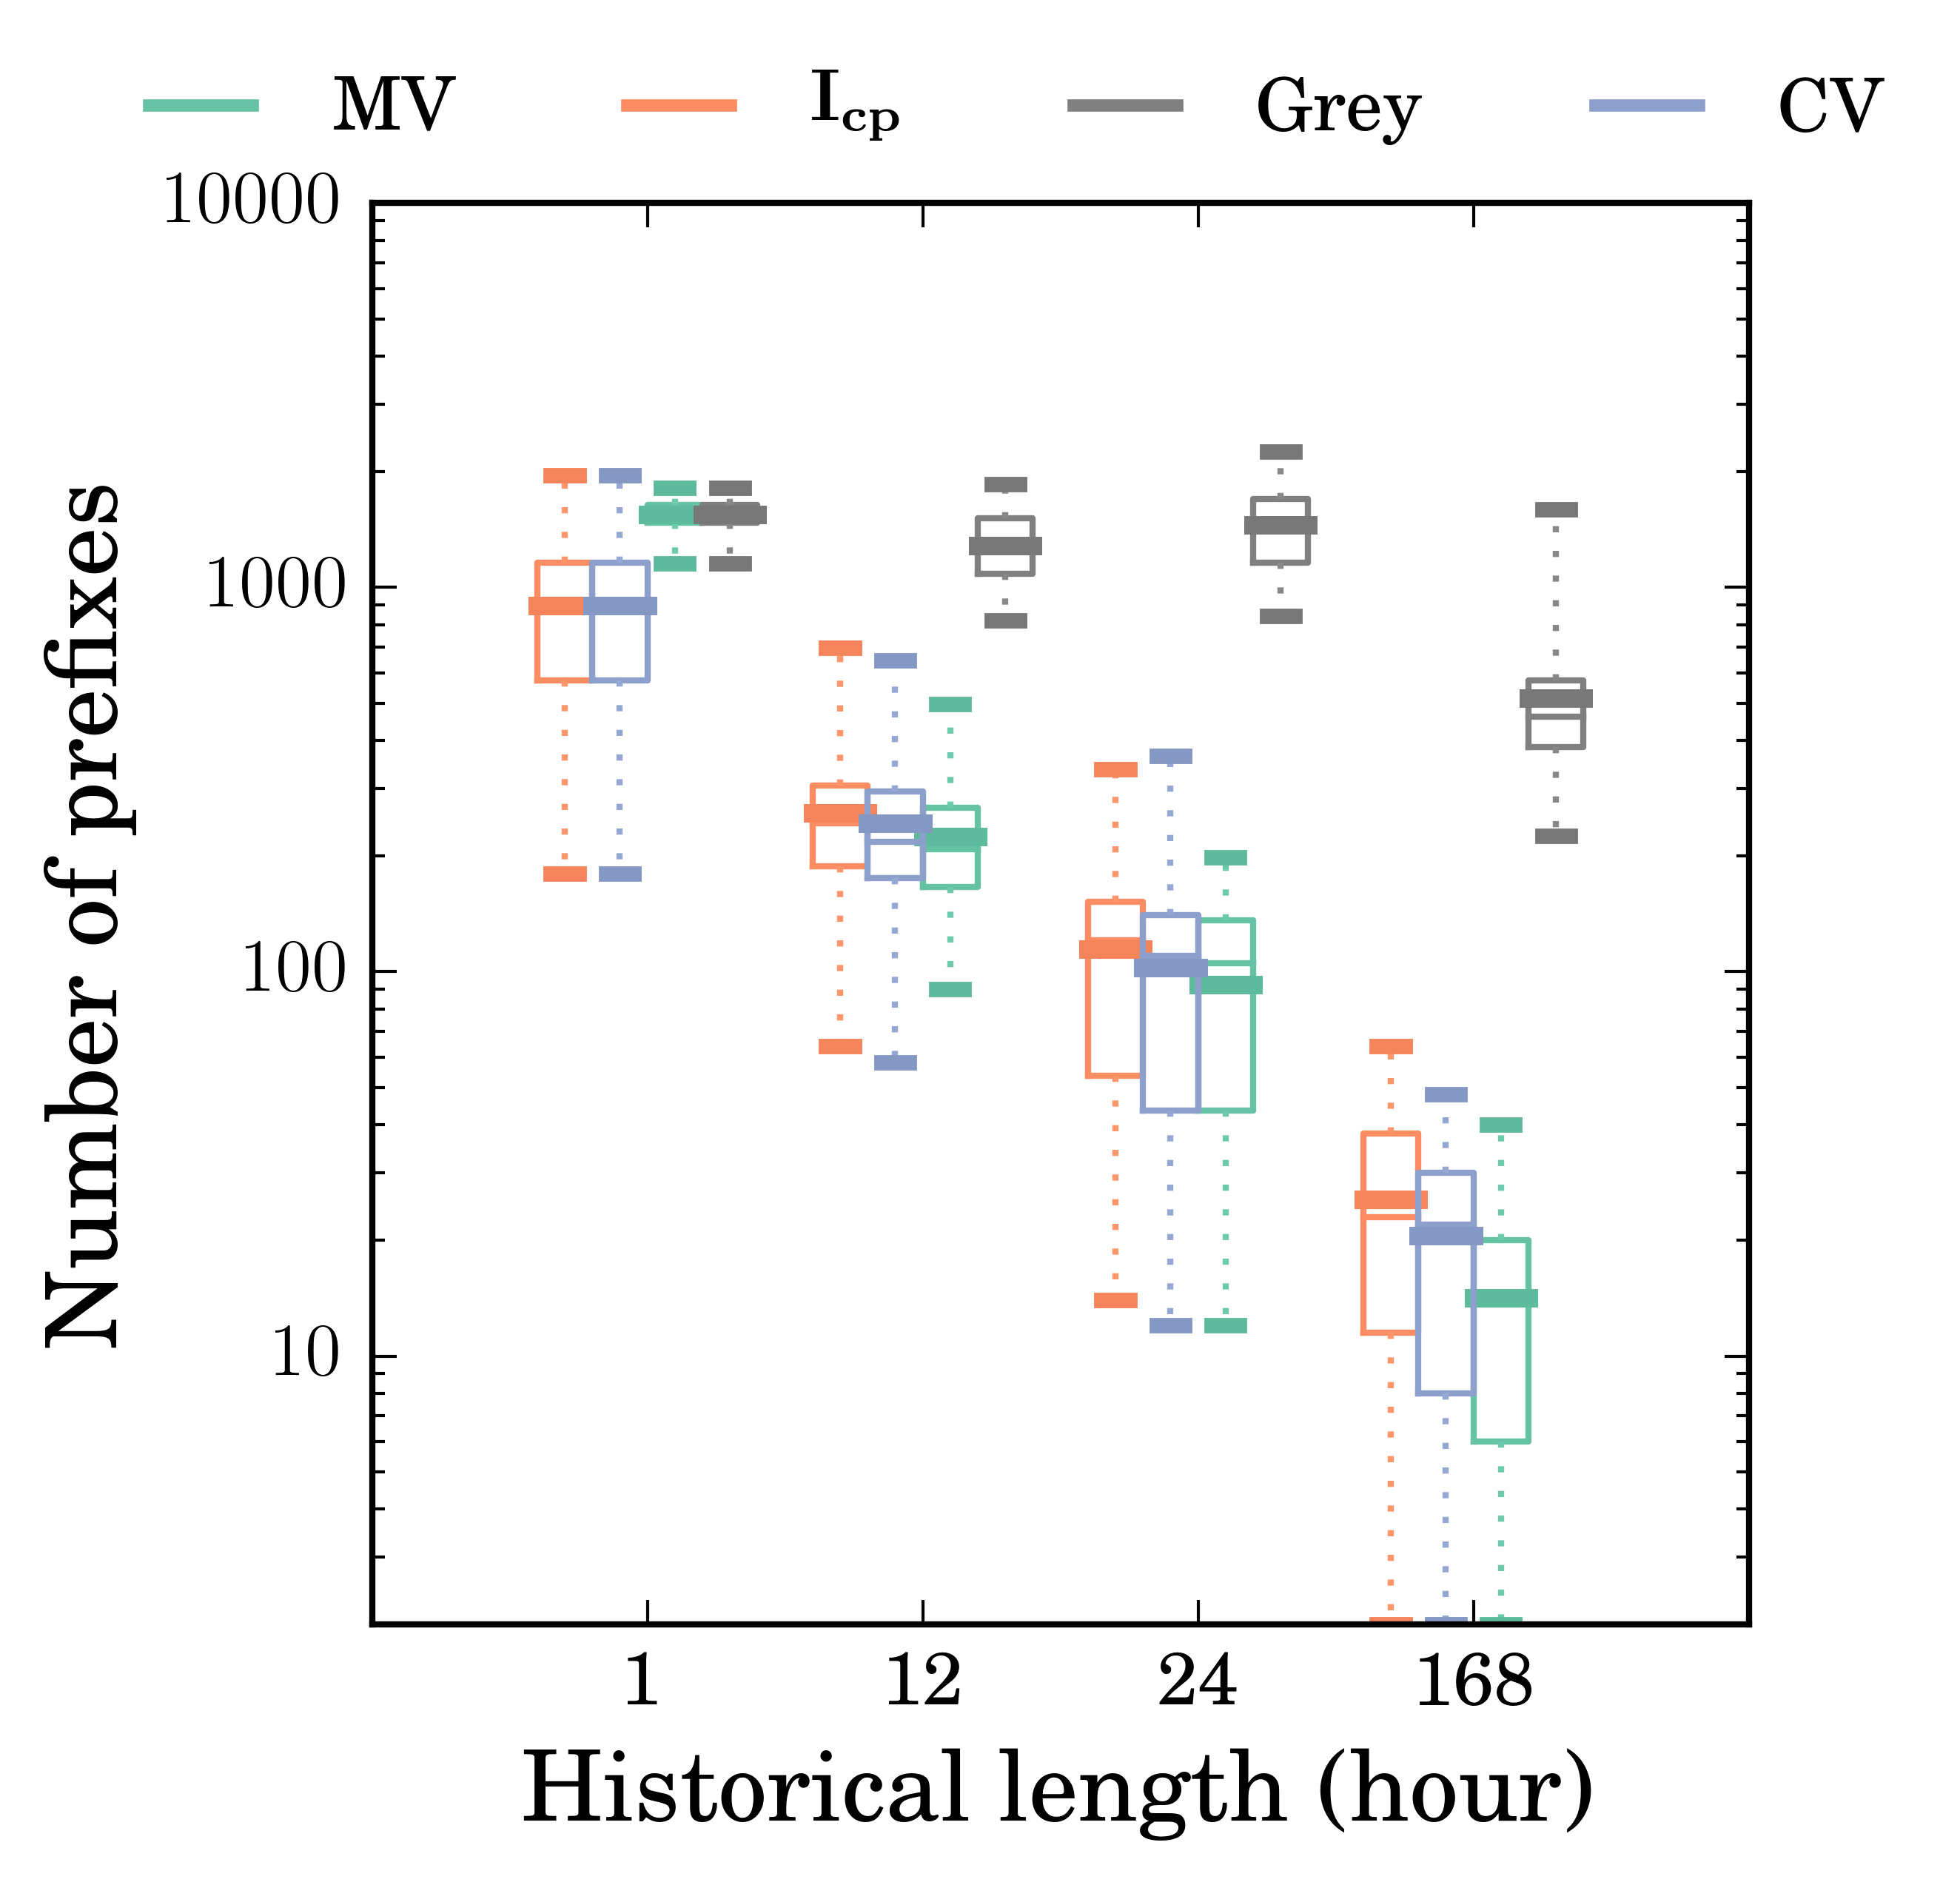
\includegraphics[width=\textwidth]{gfx/chap2/grey_churn_box_method_compare_fs_sh.png}
                \caption{SH}
                \label{fig:churn_sh}
        \end{subfigure}
        \begin{subfigure}[b]{0.48\textwidth}
                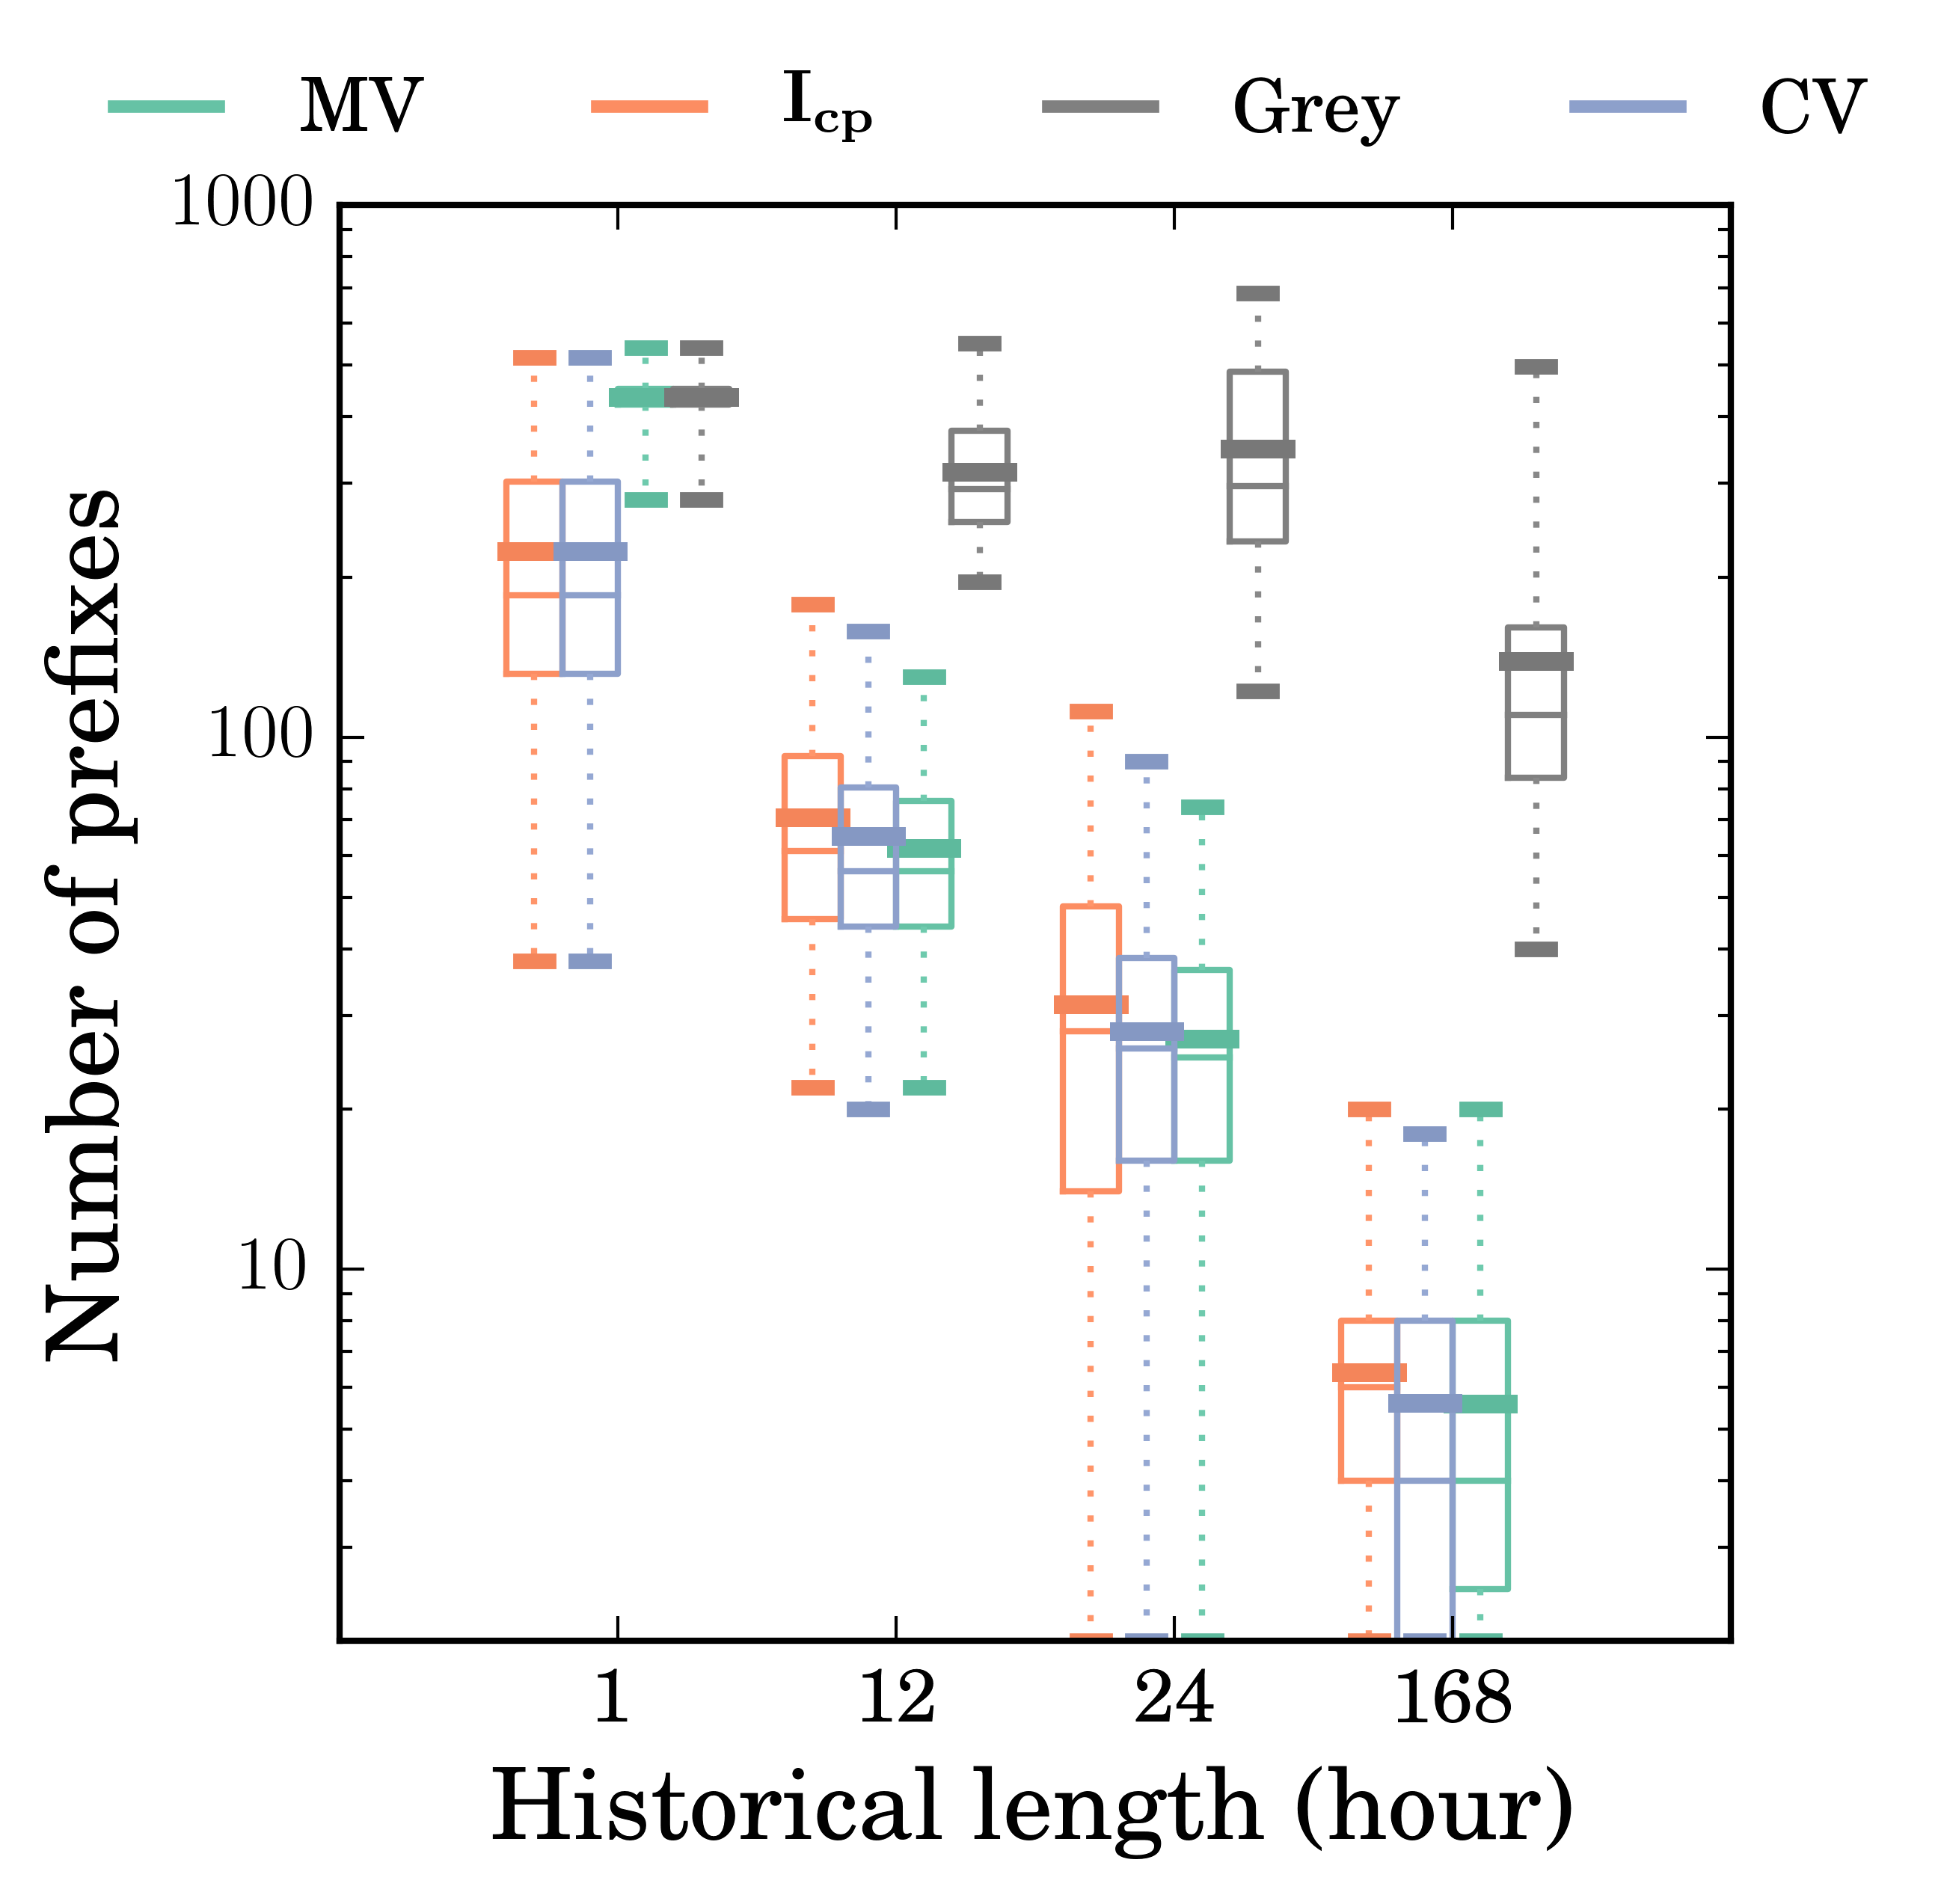
\includegraphics[width=\textwidth]{gfx/chap2/grey_churn_box_method_compare_fs_si.png}
                \caption{SI}
                \label{fig:churn_si}
        \end{subfigure}
\caption{(cont.) Hour churn of the prefix set predictively selected using historical records of different lengths.}
\label{fig:churn_cont}
\end{figure}

\marginpar{prefix churn}
Fig.~\ref{fig:churn} gives the results concerning the churn of the selection prefix set (in box-plot representation).
The churn is defined as the difference (i.e. number of new and deleted prefixes) between the new predicted set and the previous one. A high prefix churn is especially unwanted by the measurement sub-system, which aims at continuously monitoring and providing historical records of important destinations.  Sarrar et al.\ \cite{Sarrar2012} also argued that small prefix churn is very important in network architecture with decoupled forwarding and control planes, such as SDN (Software Defined Networking), as it leads to lower communication overhead.

As expected, a clear drop of the churn value can be seen when the historical length increases --- as opposed to what happens with the grey model. 
In that sense, using long historical records can be a wise choice in practice.
Furthermore, for networks with relatively few bursty traffic, e.g. SA, the mean volume coverage with last 168 hour records is extremely close to that with last 24 hour records, shown  by Fig.~\ref{fig:cvg_sa}.
Finally, for networks with highly bursty traffic, SC, using long records has the potential to obviously improve worst-case volume coverage. 

In the purpose of lowering churn, Sarrar et al.\ \cite{Sarrar2012} proposed selecting top prefixes over time bins of different lengths (ranging from 1 second to 10 minute in their FIB-caching environment). In our context, we found that the difference in mean volume coverage using record lengths larger than 1 hour is marginal, thus little gain can be expected from this method.  

%\begin{table*}[!htb]
%\centering
%\begin{tabular}{cc|cc|cc}\toprule
%\textbf{Network} & \textbf{$L$}  & \textbf{Mean Cvg.} & \textbf{Min Cvg.} & \textbf{Mean Churn} & %\textbf{Max Churn}\\
%\midrule
%SA & 24   & 93.73 & 85.32 & 32.23  & 148\\
%SB & 24   & 88.02 & 79.82 & 873.11 & 4026\\
%SC & 168  & 88.73 & 61.11 & 2.84   & 10\\
%SD & 168  & 83.22 & 69.23 & 107.06 & 1642\\
%SE & 24   & 90.51 & 78.85 & 613.72 & 1664 \\
%SF & 24   & 81.33 & 51.94 & 49.52  & 134\\
%SG & 168  & 86.44 & 52.60 & 17.24  & 48\\
%SH & 24   & 92.04 & 81.21 & 102.60 & 364\\
%SI & 24   & 87.71 & 66.75 & 28.01  & 90\\
%\bottomrule
%\end{tabular}
%\caption{Hourly volume coverage (in percentage) and churn, using \text{core} volume metric $CV$ with record length $L$ yielding the highest mean coverage.}
%\label{tab:cvg_churn}
%\end{table*}

%Among all the networks, we achieved the best mean volume coverage under $CV$ metric ($>92\%$) on SA and SH, as it can seen in Table~\ref{tab:cvg_churn}. 
%This corresponds to the fact that these two networks suffers the lest from bursty traffic.

\subsubsection{Relation between volume coverage and traffic burstiness}

\begin{figure}[!tb]
\centering
		\centering
        \begin{subfigure}[b]{0.42\textwidth}
        \centering
                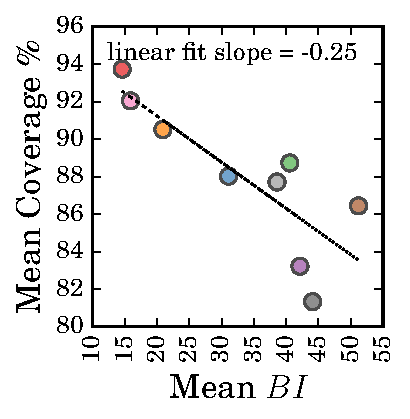
\includegraphics[width=\textwidth]{gfx/chap2/bi_cvg_mean.pdf}
                \caption{Average level}
                \label{fig:bi_cvg_mean}
        \end{subfigure}
        \hfill
        \begin{subfigure}[b]{0.53\textwidth}
                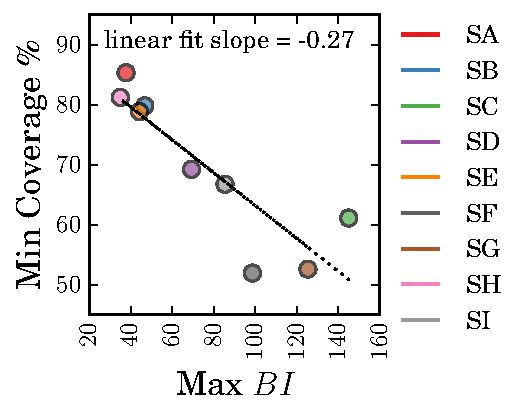
\includegraphics[width=\textwidth]{gfx/chap2/bi_cvg_worst.pdf}
                \caption{Worst case}
                \label{fig:bi_cvg_worst}
        \end{subfigure}
\caption{The relationship between burstiness index $BI$ and traffic volume coverage of selected prefix using $CV$ metric.}
\label{fig:bi_cvg}
\end{figure}

Finally, in Fig.~\ref{fig:bi_cvg} the mean/minimum coverage achieved with $CV$ metric is showed as a function of the $BI$ index. We can see that the mean (resp. minimum) coverage is inversely proportional to the mean (resp. maximum) $BI$ index. As expected, this graphic highlight the difficulty to cover a large trafic volume for networks with more bursty traffic. However, the quasi-linear curve obtained proves that $BI$ is a very meaningful metric to identify sites with bursty trafic. For large $BI$ values, it can be worthy of choosing a larger prefix set size (which was previously fixed to the weekly maximum core size), if possible. 
